\documentclass[12pt]{article}

\usepackage{float}
\usepackage{fancyhdr}
\usepackage{amsmath}
\usepackage{amsthm}
\usepackage{mathrsfs}
\usepackage{graphicx}
\usepackage{subcaption}
\usepackage{graphics}
\usepackage{wrapfig}
\usepackage{arydshln}
\usepackage{tikz}
\usepackage[
	natbib=true,
    style=numeric,
    sorting=none]{biblatex}
\addbibresource{biblio.bib}


\begin{document}
\begin{titlepage}
	\centering
	{\textsc{University of Bonn} \par}
	\vspace{1cm}
	{\Large \textsc{Lab report}\par}
	\vspace{1.5cm}
	{\huge\bfseries Setting up a radio-astronomical receiver \\
	 Setting up a twin radio interferometer\par}
	\vspace{2cm}
	{\Large\itshape Wajdee Chayeb \\
	MohammadReza Torkamani\par}
	\vfill
	Tutors:\par
	Ankur Dev\\
	Kamalpreet Kaur\\
	Pranav Limaye

	\vfill

% Bottom of the page
	{\large \today\par}
\end{titlepage}

\section{Setting up a radio-astronomical receiver}\label{S1}

In the first part of this laboratory, we examine the main properties of the components of a Heterodyne receiver to get an understanding of its main important terms and parameters. We do experiments on amplifiers, mixers, and filters to examine their functionality. Also, we conduct a calibration, simulate the influence of attenuation on signals, investigate the effect of measurement time on noise, and finally, do a radio spectroscopy using the receiver. 

\subsection{Exercise 1.1}
Radio telescopes detect very weak signals from sources and have amplifiers to amplify the amplitude of these signals so that they can be properly processed and analyzed \cite{klein}. Amplfication of Two high-frequency (HF) amplifiers and one Intermediate frequency (IF) amplifier of different bandwidths is tested. 

Input power is generated using a signal generator functioning in the continuous wave mode and set to a frequency within the bandwidth of each amplifier. The signal generator is connected to an amplifier which is connected to an HP power meter. Readings of input and output powers are recorded manually in units of dBm and plotted in Figure\ref{figure1}. To investigate the the amplification of the amplifiers, we calculate their gain which is defined as:
\begin{equation}
 \text{Gain} = 10 \log (\frac{P_{out}}{P_{in}})
\end{equation}

Where the gain is given in units of dBm, $P_{out}$ is the output power, and $P_{in}$ is the input power. 

Amplifiers do not necessarily have a linear relation between their input and output powers for all frequencies. Hence, to calculate the gain, one has to define the linear regime first. A linear fitting line using curvefit function from scipy library in Python language is used in the linear regime and the intercept is calculated \cite{scipy}. The intercept represents the gain as the relation is in dBm units (log scale). Values of the slope and gain of each amplifier along with the central frequencies used are shown in Table \ref{T1}. We calculate the errors in Table \ref{T1} from the covariance matrix given by the curvefit function. Since the power meter is not digital, there is also a source of error in reading the data points of approximately ± 0.10 dBm. 

Slopes of HF-V1 and HF-V3 are close to 1, which is expected in the linear regime. However, this is not the case for ZF-V1. This can be due to the main functionality difference of HF amplifiers and IF amplifiers as the primary role of IF amplifiers is signal conditioning and filtering for accurate demodulation, but not direct signal amplification as in the case of HF amplifiers \cite{amplifiers}. 

\begin{figure}[H]
\centering
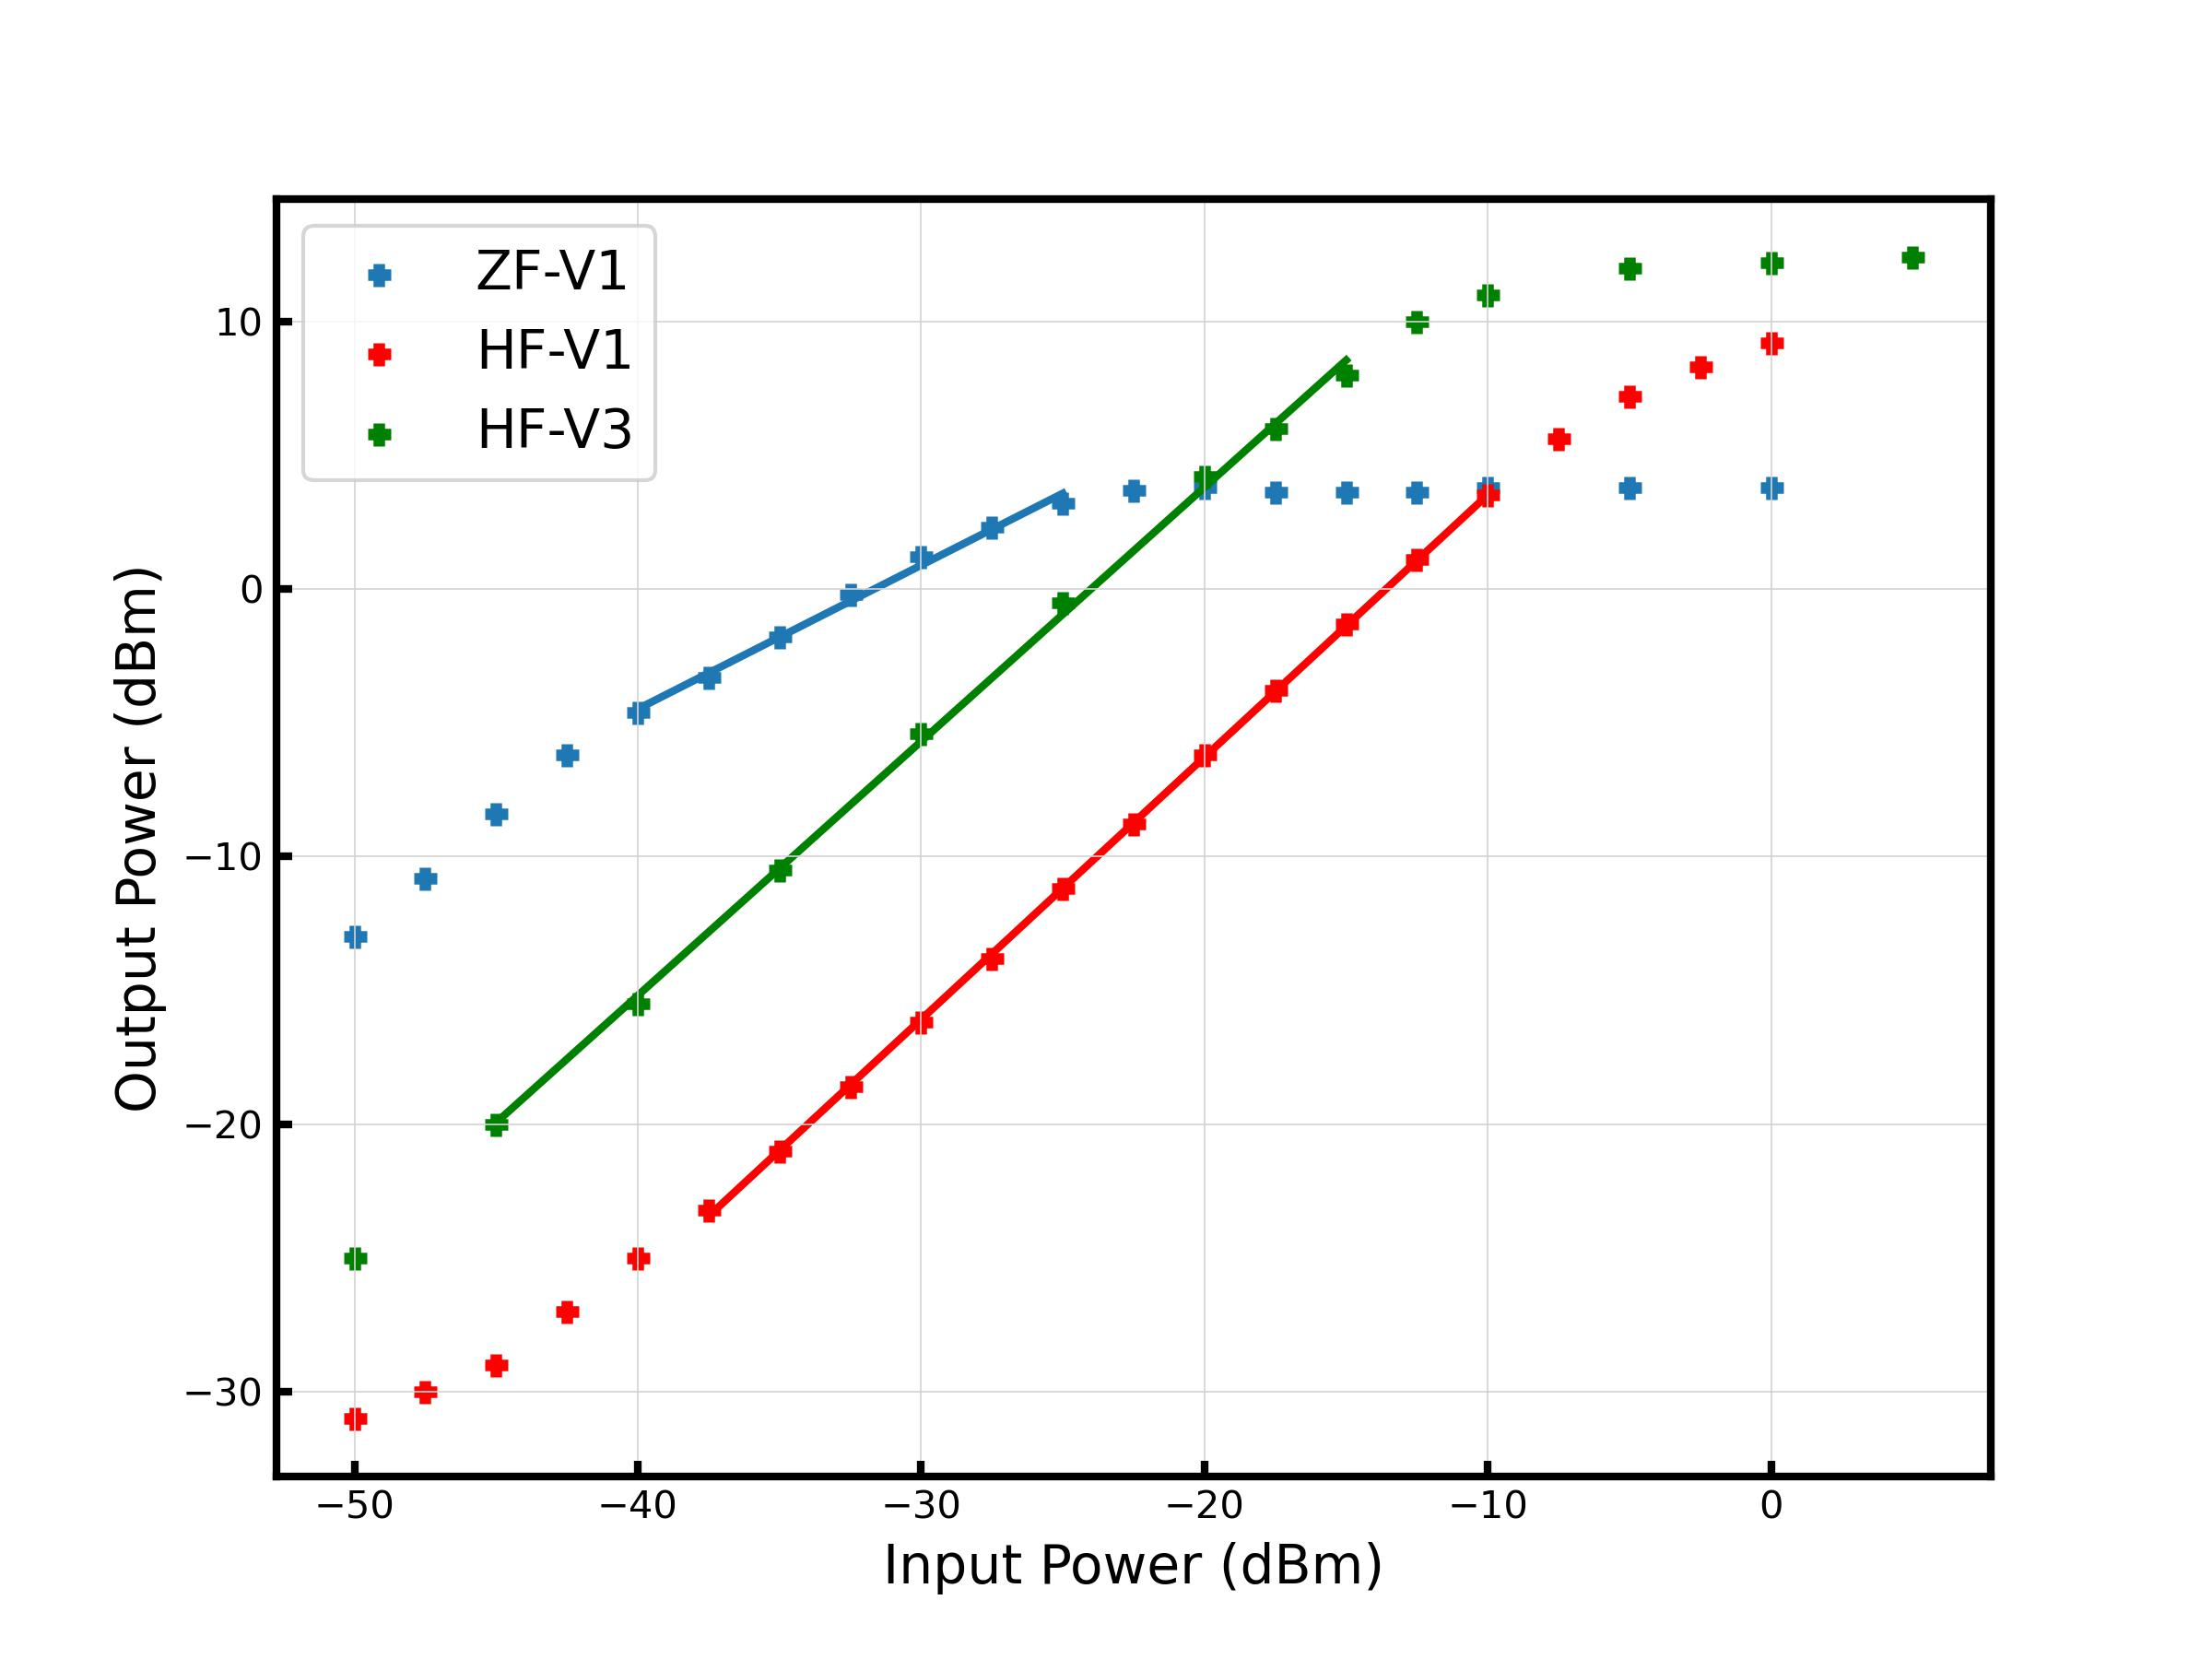
\includegraphics[scale=.5]{fig/Exercise 1.1.jpg}
\caption{Output power of amplifiers as a function of input powers}
\label{figure1}
\end{figure}


\begin{table}[H]
    \centering
    \caption{Parameters of the three amplifiers}
    \label{T1}
    \begin{tabular}{c |c |c |c}
        \hline
        \hline
        Amplifier & ZF-V1 & HF-V1 & HF-V3\\
        \hline
         Central Frequency & 500 MHz & 2.5 GHz & 3 GHz \\

        Slope & $0.698 \pm 0.029$ & $0.980 \pm 0.004$ & $0.950 \pm 0.013$ \\
     
        Gain & $22.687 \pm 1.178$ & $13.323 \pm 0.093$ & $22.795 \pm 0.400$ \\
        \hline
    \end{tabular}
\end{table}
\subsection{Exercise 1.2}
Filters are used to eliminate unwanted frequencies from the received signals as the band of interest in observation is narrow \cite{klein}. Some parameters that determine the functionality of filters are the bandwidth, insertion loss, and adjacent band rejection, which are defined in \cite{lecturenote}. Here, we measure the output powers of two filters, HF-F1 and ZF-F1, and calculate those parameters.  A signal is generated using a signal generator with a power of 5 dBm and fed to a filter connected to a power meter. The input frequency is varied and the output power is recorded manually. 
The data of each filter is plotted in Figure \ref{figure2}. The black lines correspond to the maximum power which has attenuated by 3dB and is used to determine the bandwidth of a filter. A linear fitting is done on the plateaus, right, and left sidebands. The fitting parameters are described in Table \ref{T2} and \ref{T3}. 

A bandwith is the range of frequencies over which the filter allows signals to pass with minimal power loss or attenuation. It is the difference between the upper and lower cutoff frequencies of the filter, where the signal level is reduced or attenuated compared to the passband \cite{bandwidth}. To calculate the bandwidths, we first start by calculating the mean maximum output power with its error. Then, we calculate the -3 dBm cut-off line by subtracting 3 dBm from the maximum output power to get the half-power bandwidth. Next, we find the corresponding frequencies of the two data points where the -3 dBm line intersects with our curve. The resulting bandwidth of each filter are shown in Table \ref{T4}. 


A conversion loss is the reduction of the output power compared to the input signal expressed in units of dBm and calculated according to the following formula \cite{mixers}:

\begin{equation}
 \text{Insertion Loss (IL)} = P_{in} - P_{out} 
\end{equation}

Where $P_{in}$ is the input power in dBm used, and $P_{out}$ is the output power in dBm recorded at the central frequency. Values of Insertion loss of the two filters are also shown in Table \ref{T4}. 

Adjacent band rejection is a measure of a device's  ability to reject or attenuate signals from adjacent frequency bands or channels \cite{mixers}. It is an important parameter which is important to determine especially in scenarios where multiple frequency channels or signals are closely spaced. For calculating the adjacent-band rejection, we use the frequency regions with a -60 dBm cut-off. Values are shown in Table \ref{T4}.  
\begin{figure}[H]
     \centering
     \begin{subfigure}{.45\textwidth}
         \caption{HF-F1}
        \label{fig1.21}
         \centering
         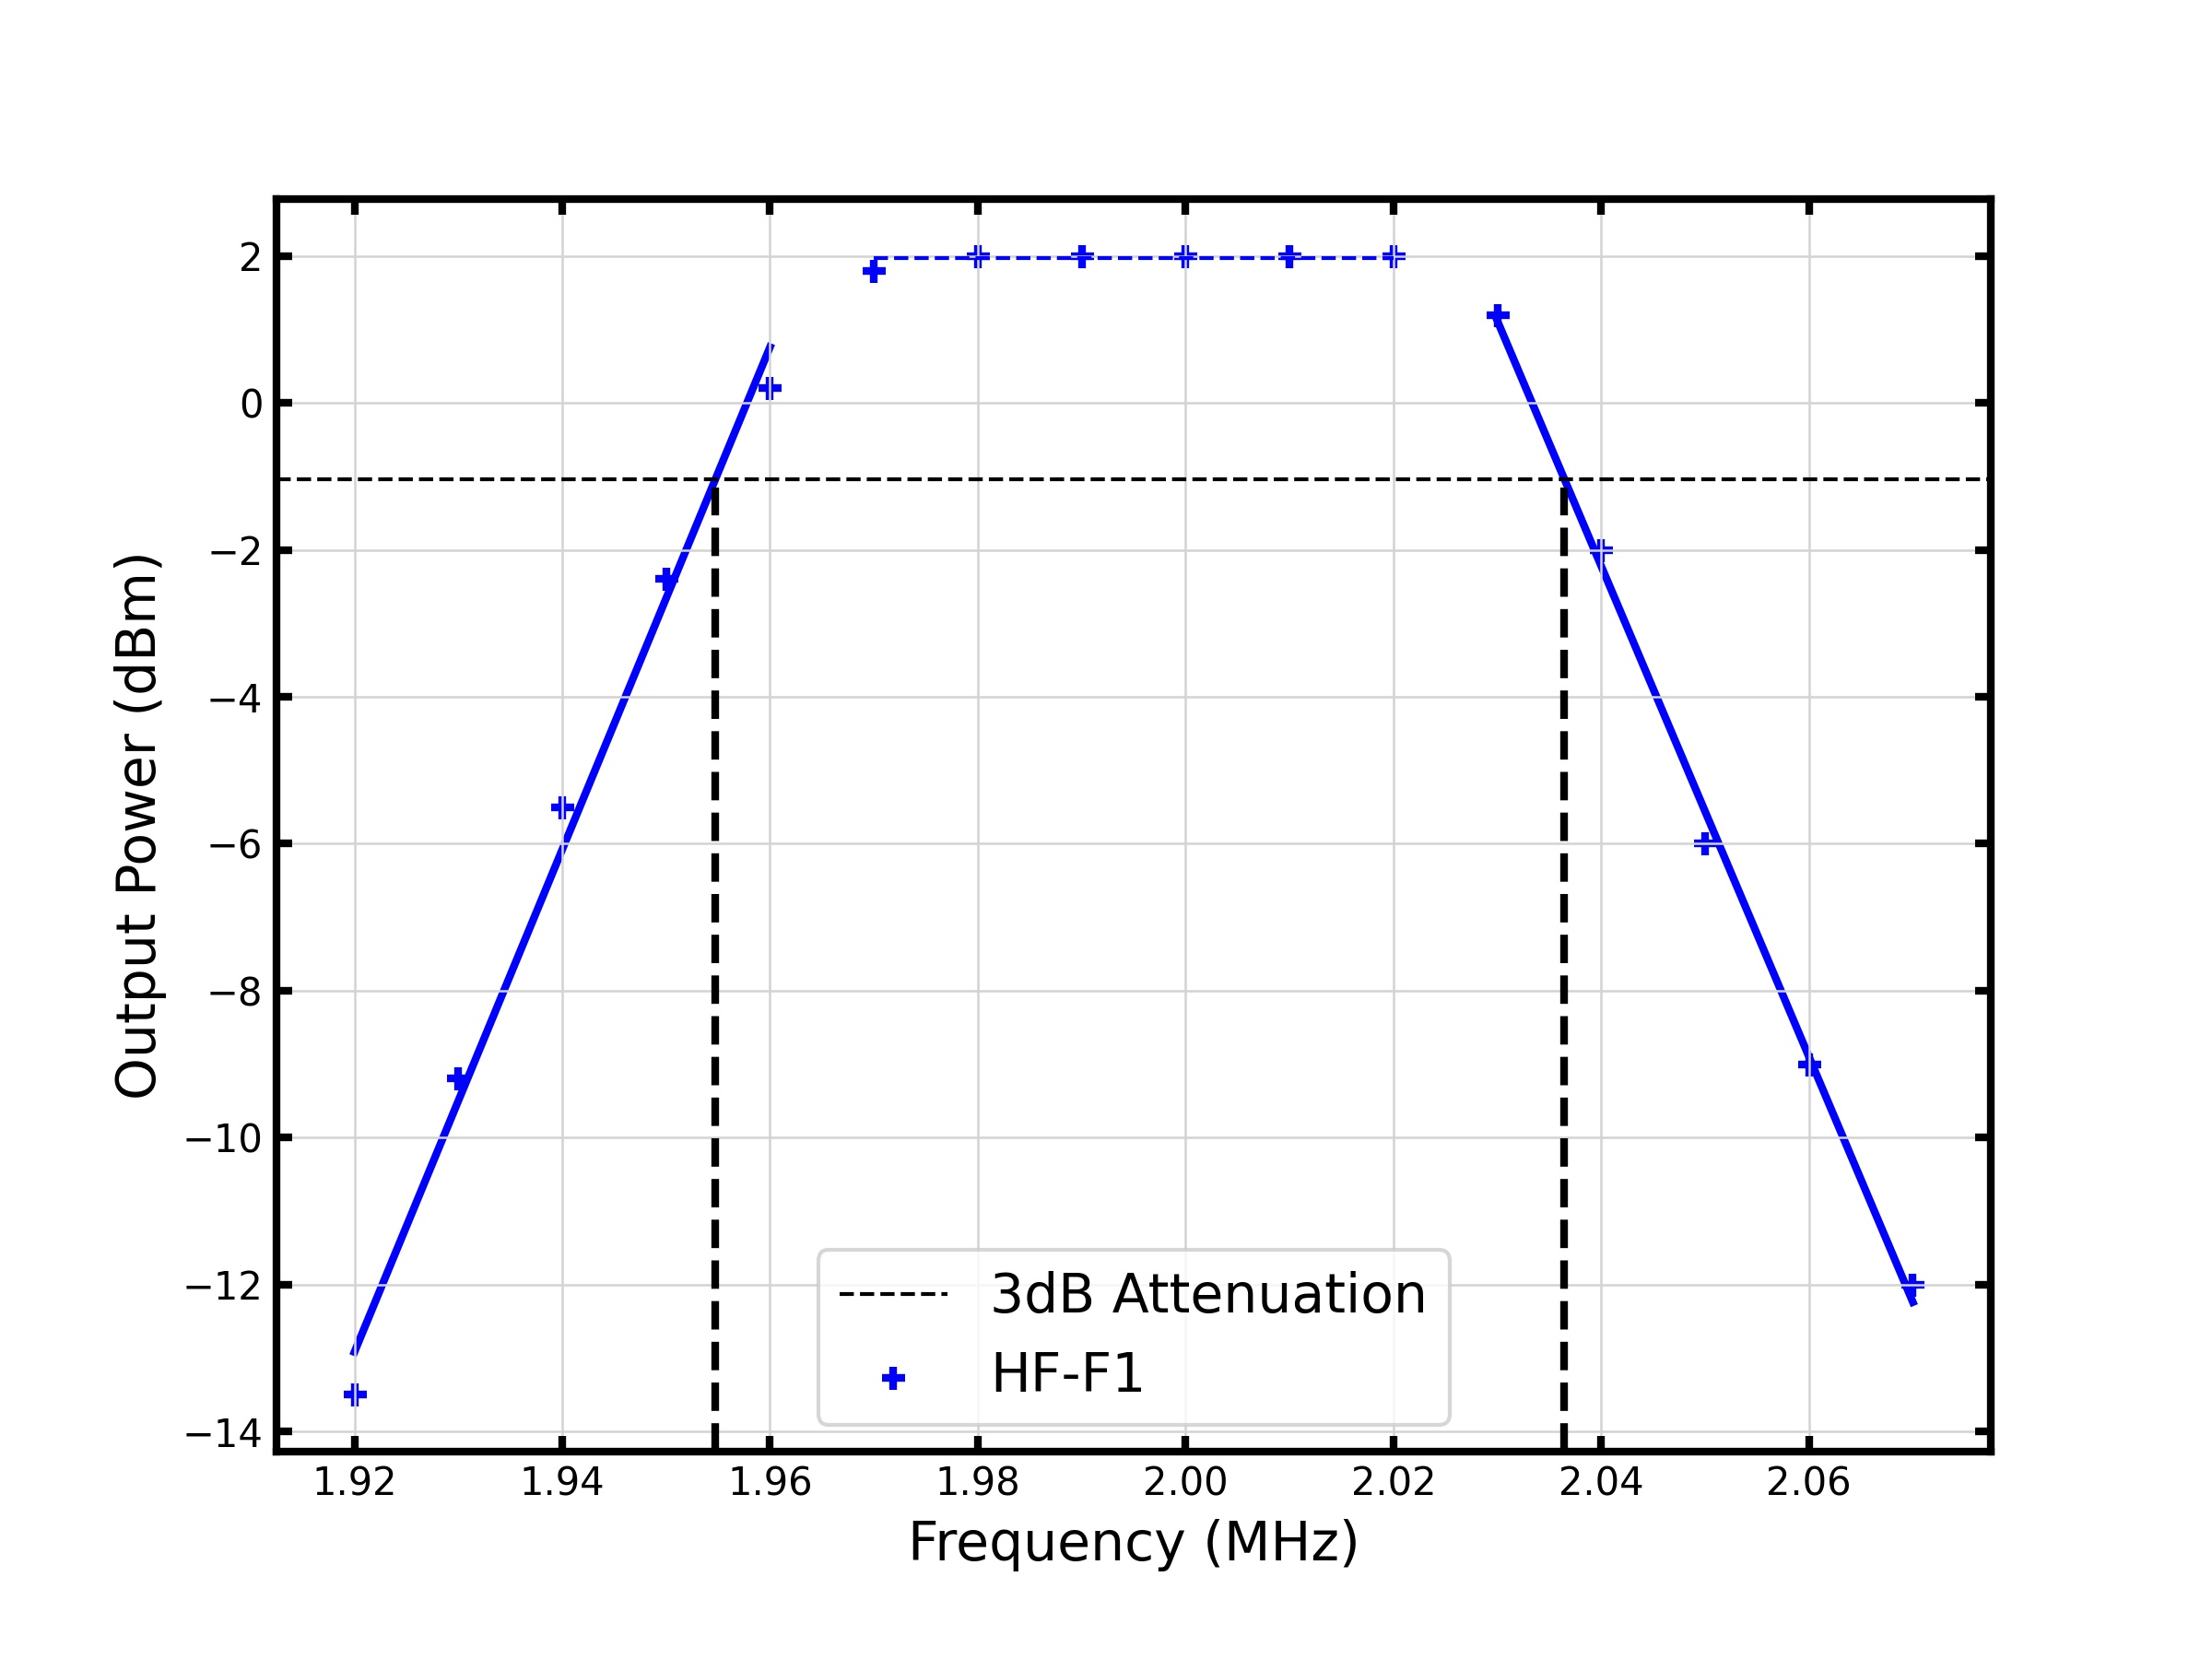
\includegraphics[width=\textwidth]{fig/Exercise 1.21.jpg}
     \end{subfigure}
     \hfill
     \begin{subfigure}{.45\textwidth}
         \centering
         \caption{ZF-F1}
         \label{fig1.22}
         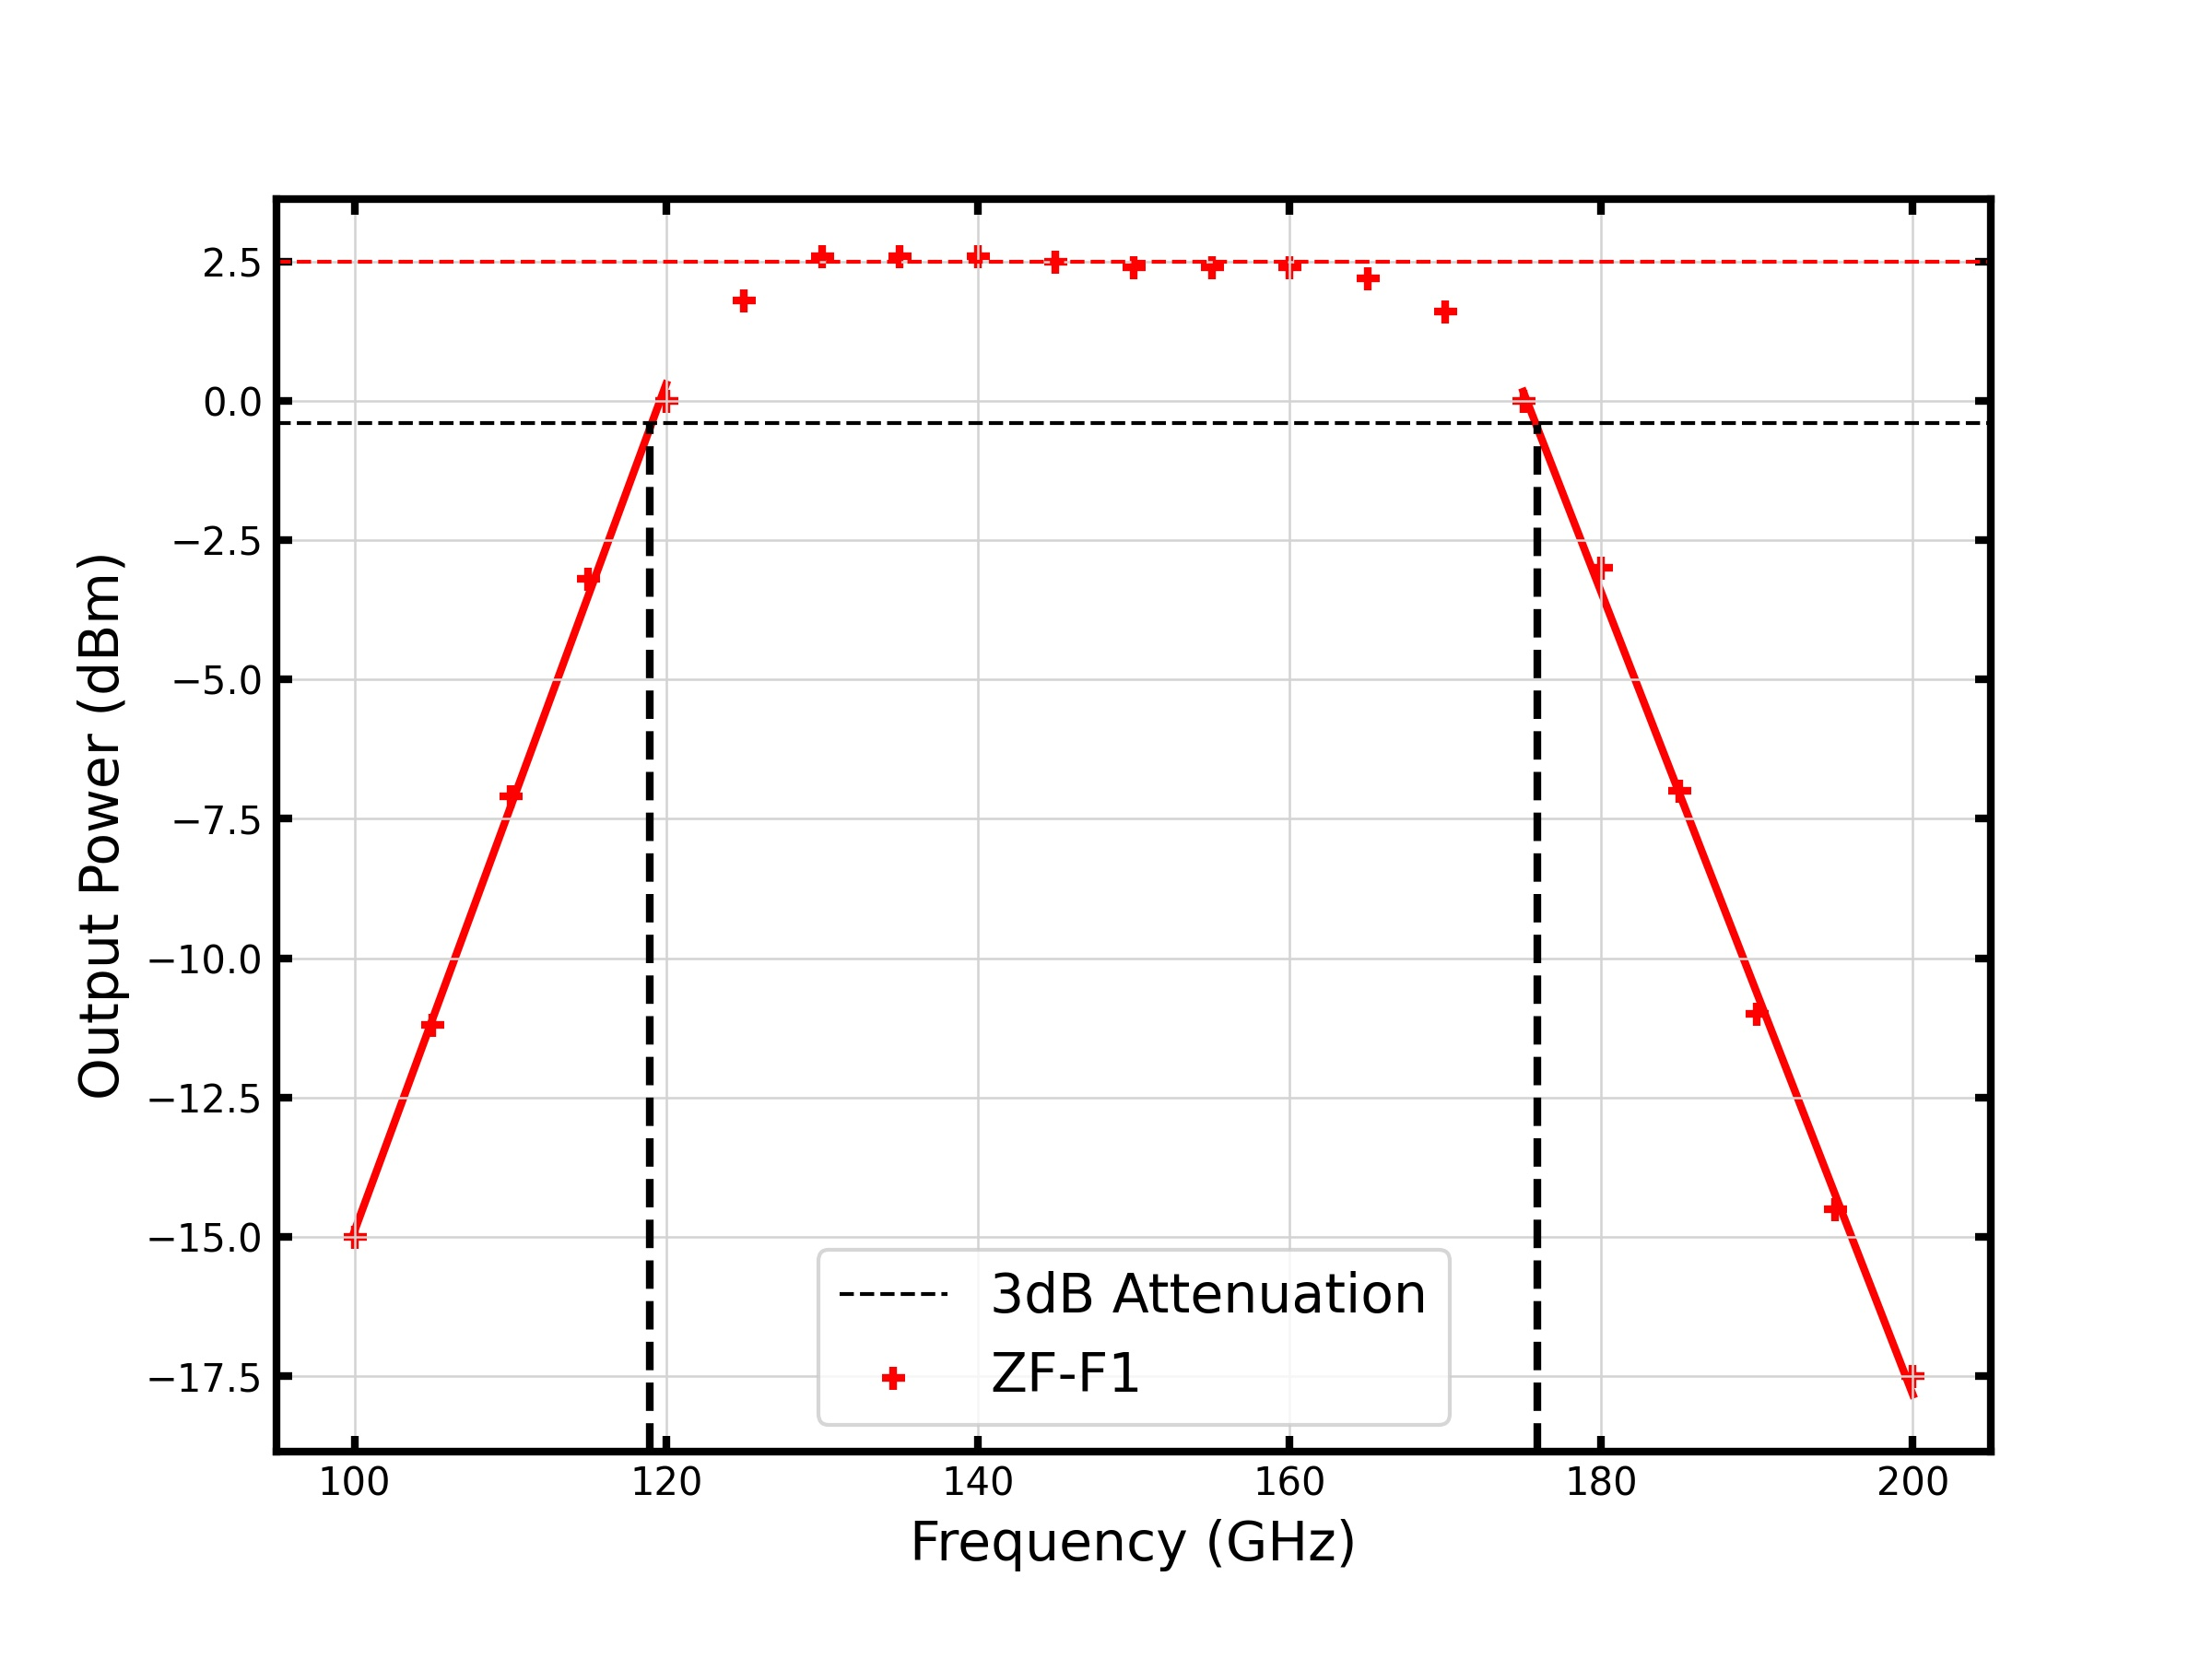
\includegraphics[width=\textwidth]{fig/Exercise 1.22.jpg}
     \end{subfigure}
     \caption{Output power of filters against frequency}
     \label{figure2}
 \end{figure}
 
\begin{table}[H]
    \centering
    \caption{Filters fitting Parameters of HF-F1}
    \label{T2}
    \begin{tabular}{c |c |c }
        \hline
        \hline
         & Slope & Intercept  \\
        \hline
        Plateau & 2.857 ± 1.650 & -3.733 ± 3.291\\
        
        left Sideband & 342.000 ± 19.528 & -669.560 ± 37.885\\
        Right Sideband & -334.000 ± 10.263  & 679.140 ± 21.040 \\

        \hline
    \end{tabular}

\end{table}

\begin{table}[H]
    \centering
    \caption{Filters fitting Parameters of ZFF1}
    \label{T3}
    \begin{tabular}{c |c |c }
        \hline
        \hline
         & Slope & Intercept\\
        \hline
        Plateau & -0.009 ± 0.002 & 3.743 ± 0.227\\
        
        left Sideband & 0.760 ± 0.018 & -90.900 ± 1.972\\
        Right Sideband & -0.720 ± 0.017  & 126.167 ± 3.277 \\
        \hline
    \end{tabular}

\end{table}


\begin{table}[H]
    \centering
    \caption{Filters measured parameters}
    \label{T4}
    \begin{tabular}{c |c |c }
    
        \hline
        \hline
         Filter & HF-F1 & ZF-F1\\
        \hline
        Central Frequency [GHz] & 1.99  & 0.15\\ 
        Mean Maximum Power [dBm] & $1.97 \pm 0.03$ & $2.50 \pm 0.04$ \\
        Insertion Loss [dBm] &  $3.03 \pm 0.03$ & $2.50 \pm 0.04$ \\
        Adjacent Band Rejection [GHz] / [MHz]& $1.78 \pm 0.23$ & $40.66 \pm 7.27$\\ 
        Bandwidth [GHz] / [MHz]& $0.082\pm 0.001$ & $56.978 \pm 11.884$\\
        \hline

        \end{tabular}
\end{table}


\subsection{Exercise 1.3}

When displaying the bandpass of the HF-F1 filter on the oscilloscope, we see a Gaussian-like shape when the filter frequency aligns with the filter's peak response. As we vary the central frequency of the filter, we see the position of the peak shifting. The peak is not a perfect Gaussian because the oscilloscope shows the voltage in mW units. 

 \begin{figure}[H]
\centering
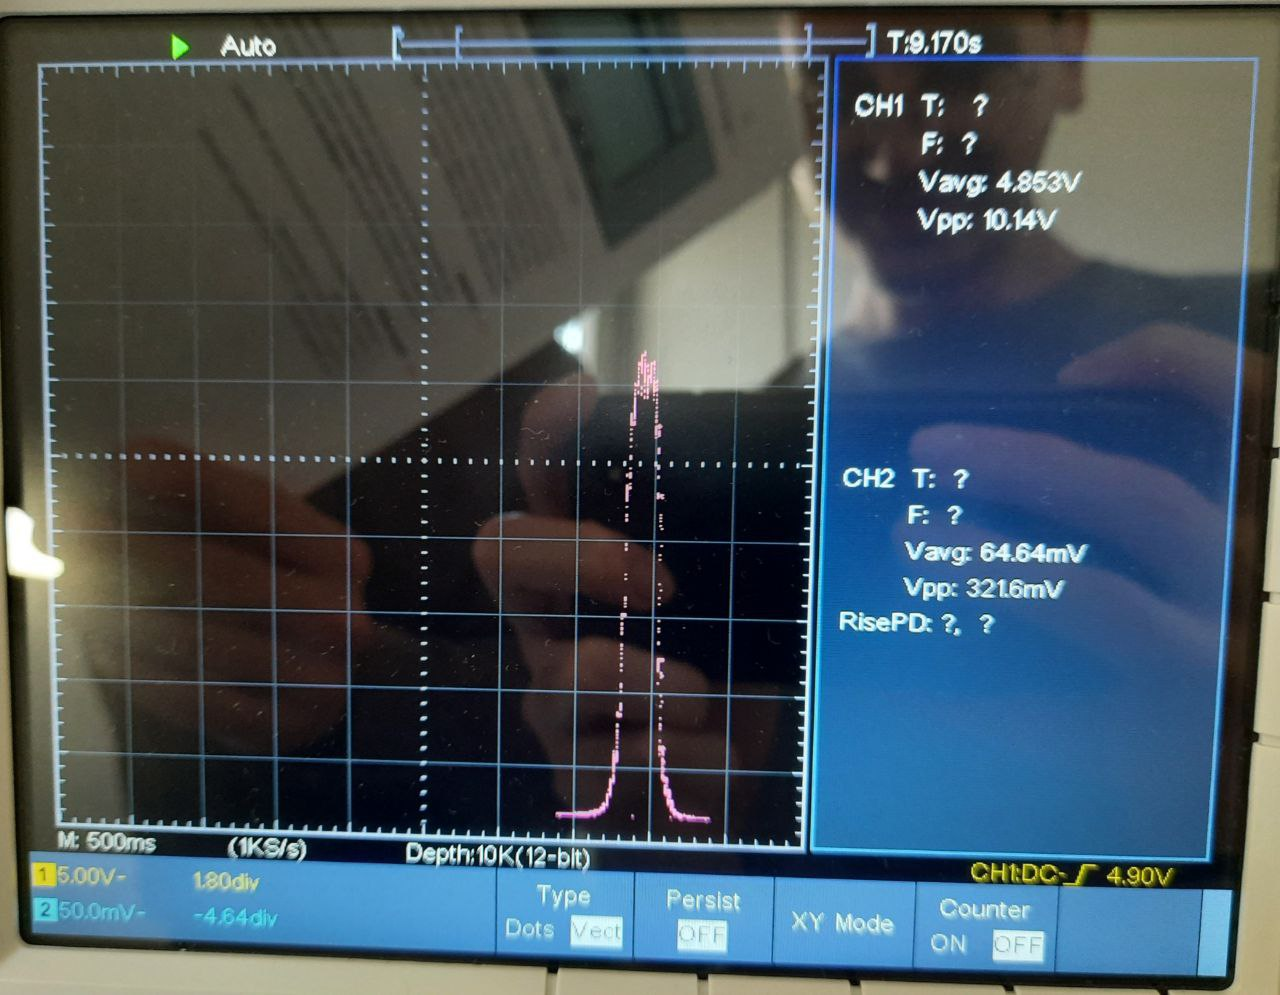
\includegraphics[scale=.2]{fig/Exercise 1.3.jpg}
\caption{Bandpass of the filter HF-F1 at central frequency }
\label{fig1.3}
\end{figure}

\subsection{Exercise 1.4}


A mixer applies the principle of heterodyning where a high-frequency signal is down-converted to a lower frequency by mixing it with a signal generated by a local oscillator (LO) \cite{klein}. The two frequencies are summed and subtracted from each other resulting in two frequencies. The summation frequency is filtered out, while the other frequency (also known as the intermediate frequency) is kept for further processing \cite{klein}. 

We prove the linearity between the input and output power of a mixer by varying the input power, recording the output power using a power meter, and plotting the data. The local oscillator (LO) is set to a power of 13 dBm and a frequency of 2.45 GHz, while the signal generator is set to a power of 0 dBm at a 2.3 GHz frequency.

The results are plotted in Figure \ref{fig1.4}. A clear linear relation is seen confirming our expectation with a value of slope close to 1. The fitting parameters are shown in Table \ref{T5}. We then calculate the conversion loss which is caused due to demodulation effects \cite{mixers}. Here, A conversion loss is the y-axis intercept as the plot is in log scale. From our results, we conclude that the mixer reduced the input power of a factor of almost 10 dB, in other words, the output power is approximately 80\% weaker than the output power. Thus, an additional amplifier is needed to compensate for the power loss and this is used in a superheterodyne receiver and agrees with the scheme illustrated in Figure \ref{fig1.3} in the lab manual \cite{lecturenote}

\begin{table}[H]
    \centering
    \caption{Mixer Parameters}
    \label{T5}
    \begin{tabular}{c |c}
        \hline
        \hline
        Slope & Intercept (Conversion Loss) \\
        \hline
        
         0.947 ± 0.006 & -10.157 ± 0.021\\
        \hline
    \end{tabular}
\end{table}

\begin{figure}[H]
\centering
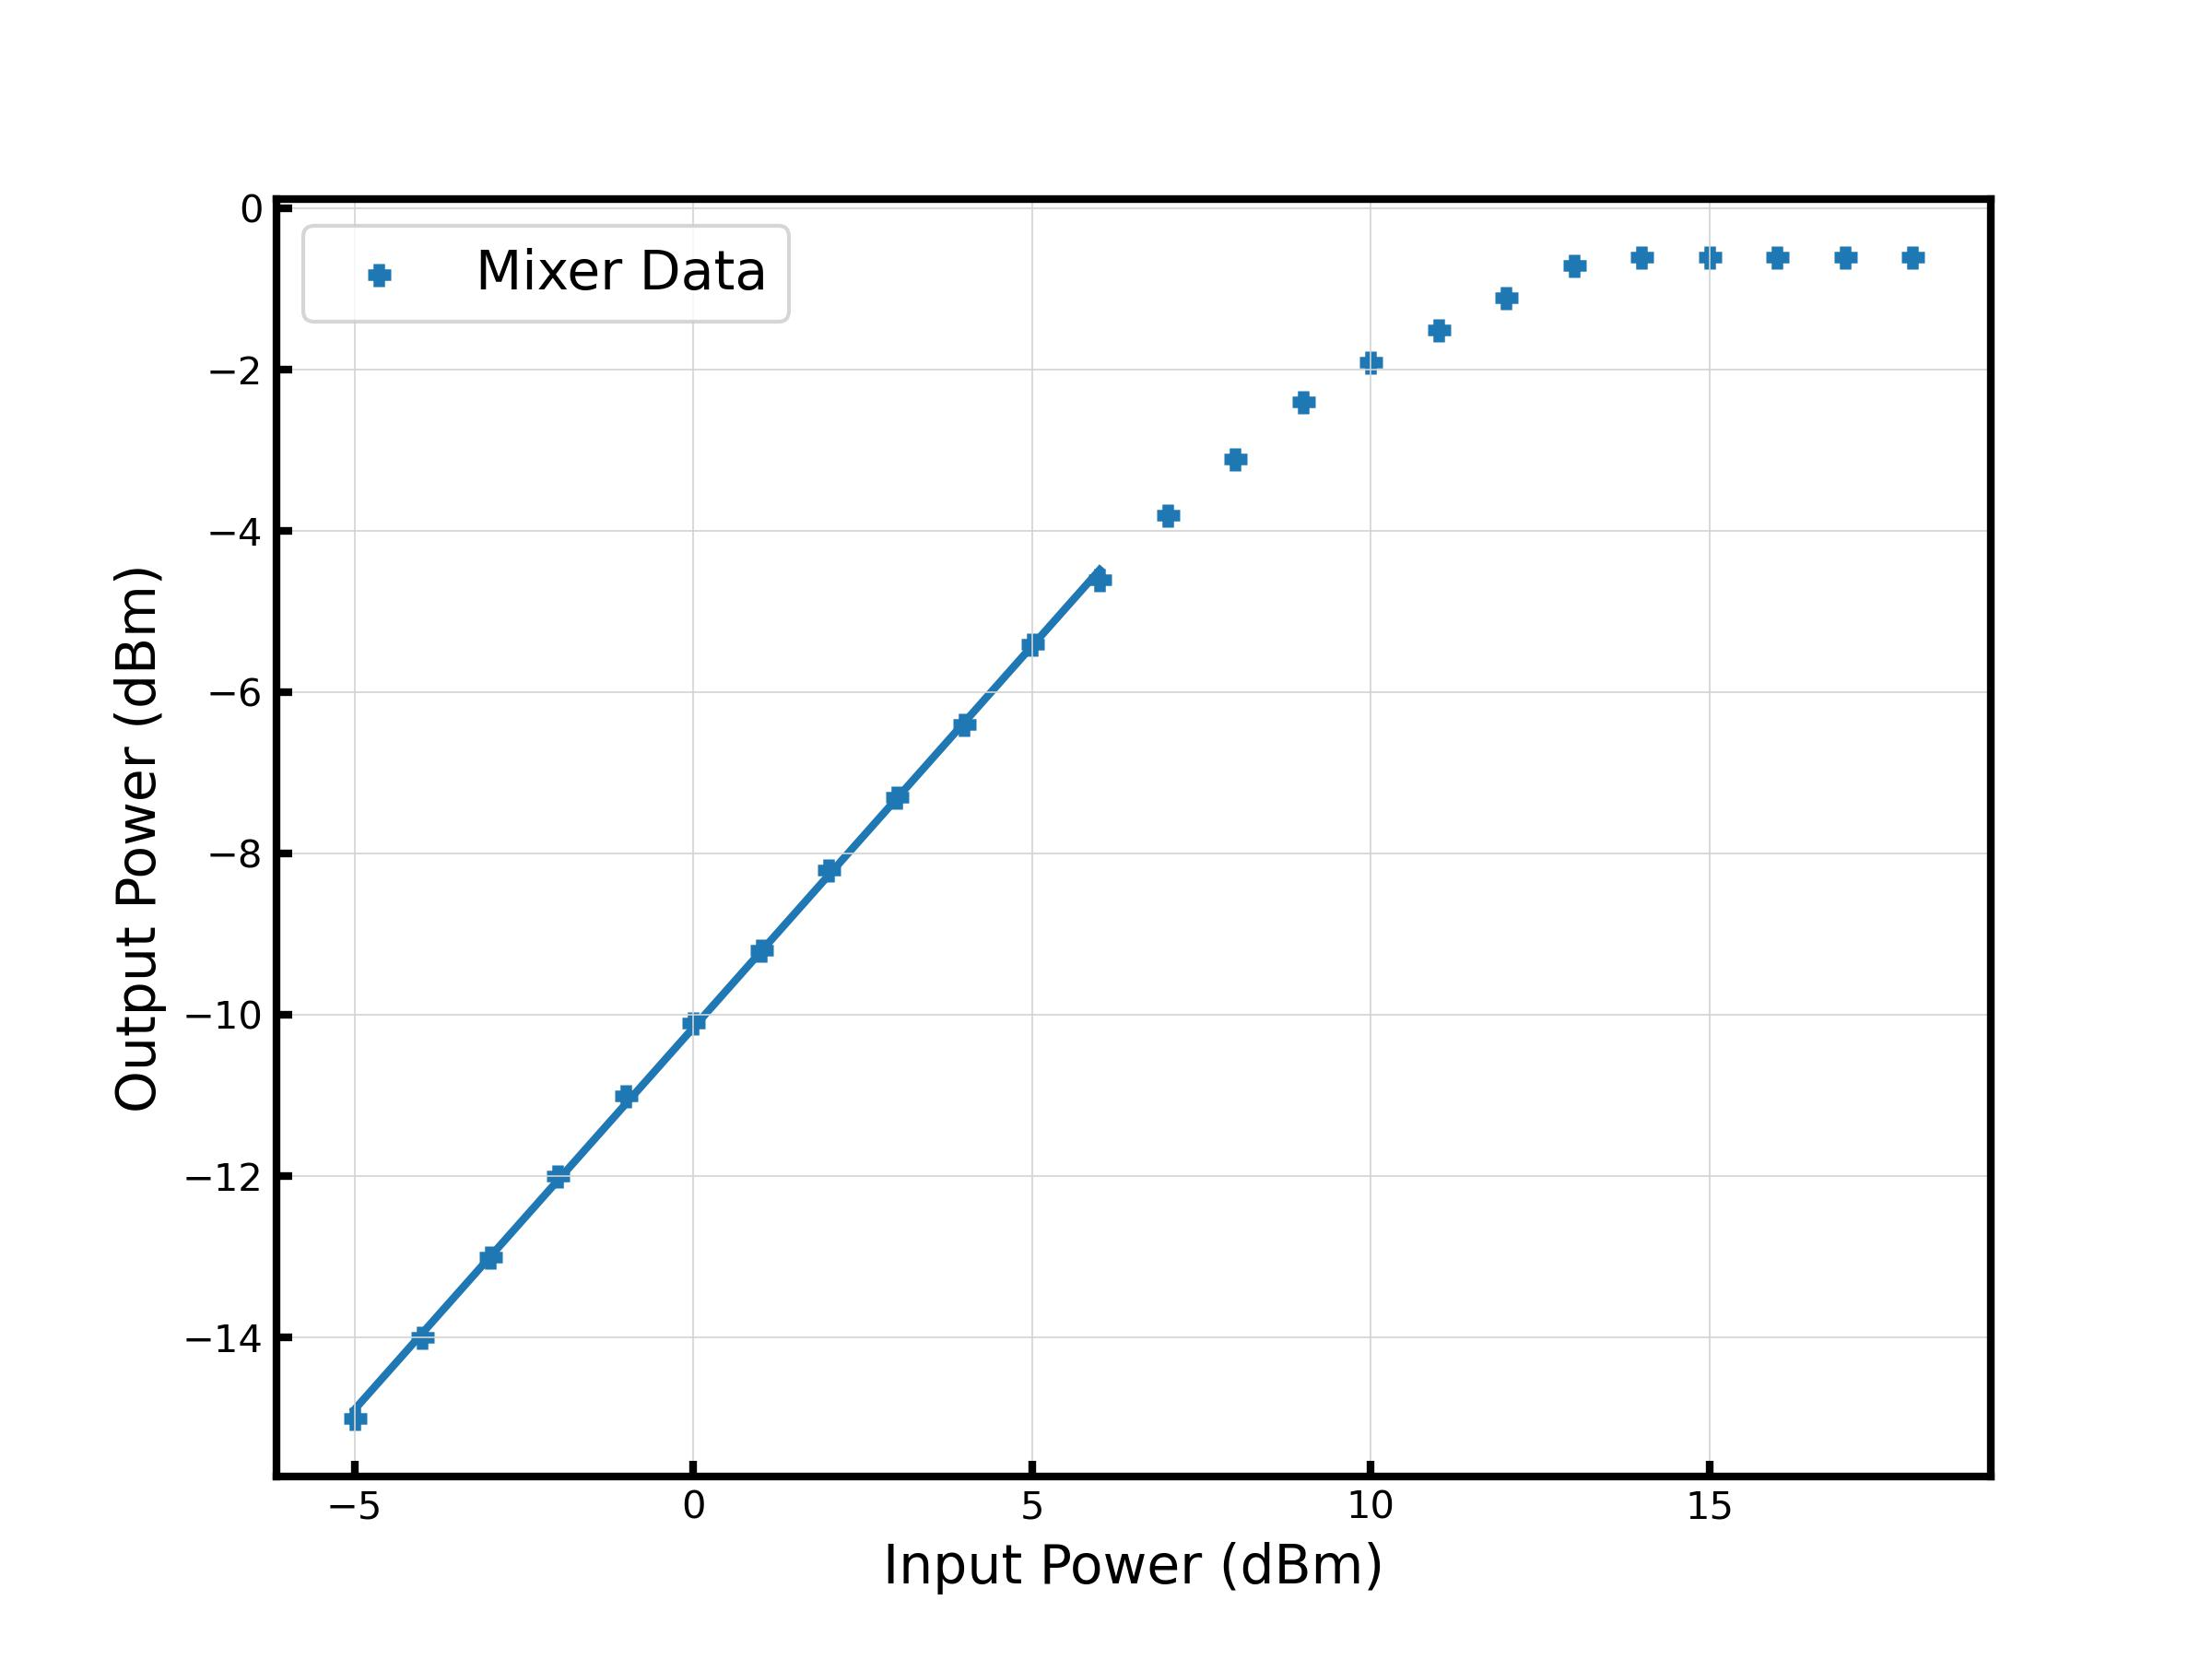
\includegraphics[scale=.5]{fig/Exercise 1.4.jpg}
\caption{Output power of the mixer as a function of input powers}
\label{fig1.4}
\end{figure}

\subsection{Exercise 1.5}
Two power measurements at known temperatures are needed for the receiver temperature to be determined and the calibration process to be done \cite{klein}. A resistor providing an input noise is used for a measurement that involves two temperature conditions: room temperature (299 K) and cooled temperature (77 K), known as Hot-cold calibration \cite{klein}. The measurement reading is conducted using the Gqrx SDR software. The process begins at room temperature, and the resistor (50 $\Omega$) is then cooled by immersion in liquid nitrogen. The measurement continues once the resistor has sufficiently cooled. The  data is plotted in Figure \ref{fig1.51} and the average for hot and cold powers are calculated as described in Table \ref{T6}. The resulting hot and cold powers are plotted against their corresponding temperature in Figure \ref{fig1.52}. When converting the units from dBm to mW, we calculate the errors of power in mW using the following conversion factor:

\begin{equation}
\Delta p_{mW} = ln(10)\times 10^{\frac{p_{dBm}}{10}}
\Delta p_{dBm} 
\end{equation}


\begin{table}[H]
    \centering
    \caption{Hot-Cold Calibration Parameters}
    \label{T6}
    \begin{tabular}{c| c c}
        \hline
        \hline
        Temperature (Kelvin) & $P_{out}[\mathrm{dBm}]$ & $P_{out}[\mathrm{mW}]$ \\
        \hline
        
        $299 \pm 0.5$ & $-30.998 \pm 0.004$ & $0.000795 \pm 0.000007$\\
        $77 \pm 5$ & $-32.882 \pm 0.002$ & $0.000515 \pm 0.000003$\\
        \hline
    \end{tabular}

\end{table}



\begin{figure}[H]
\centering
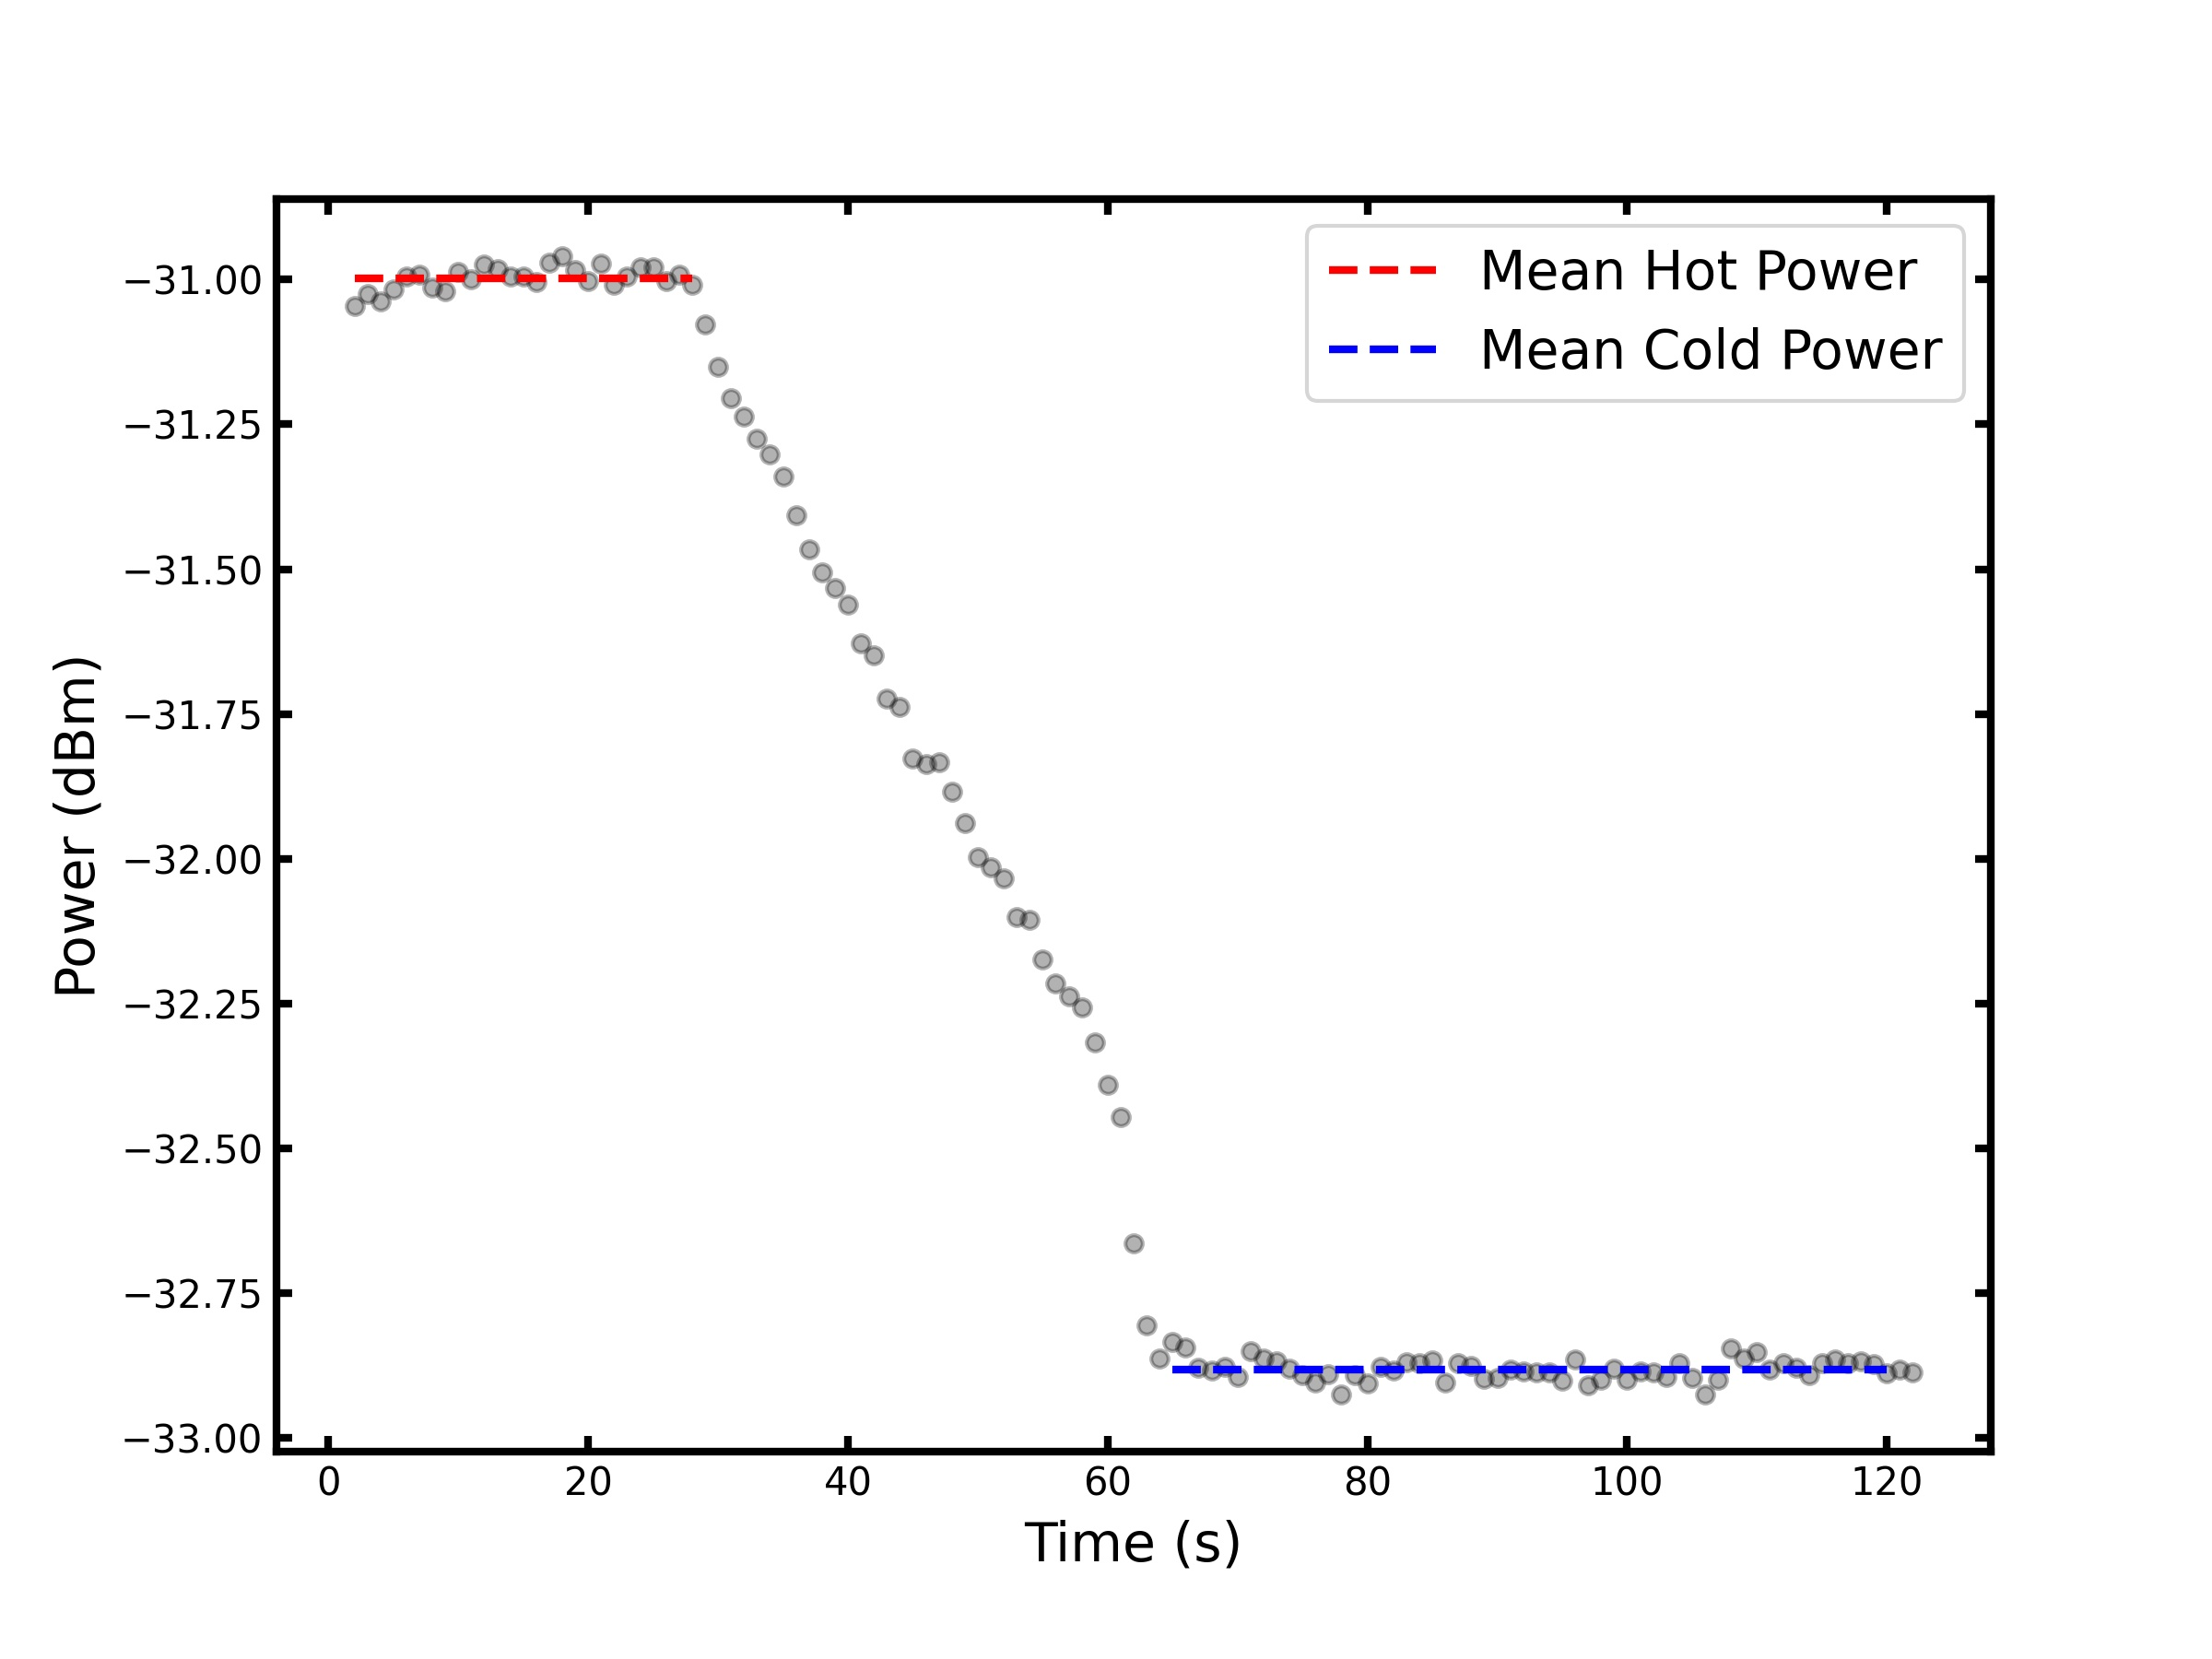
\includegraphics[scale=.5]{fig/Exercise_5_1.jpg}
\caption{Output power as a function of time for Hot-Cold calibration}
\label{fig1.51}
\end{figure}

With the parameters given in the previous table, the receiver temperature can be calculated using the following formula \cite{radiometereq}:

\begin{equation}
\ T_{reciever} = P_{cold}\dfrac{T_{hot} - T_{cold}}{T_{hot} - T_{cold}} - T_{cold}
\end{equation}

As a result, we get $T_{rec} = (332 \pm 32)$ K. We also determine the receiver temperature graphically using a linear function, which is interpolated between the two data points shown in Figure \ref{fig1.52}. The linear function has the form:

\begin{equation}
    P_{out} = (1.2603 \times 10^{-6} \cdot T  + 0.0004) mW
\end{equation}

\begin{figure}[H]
\centering
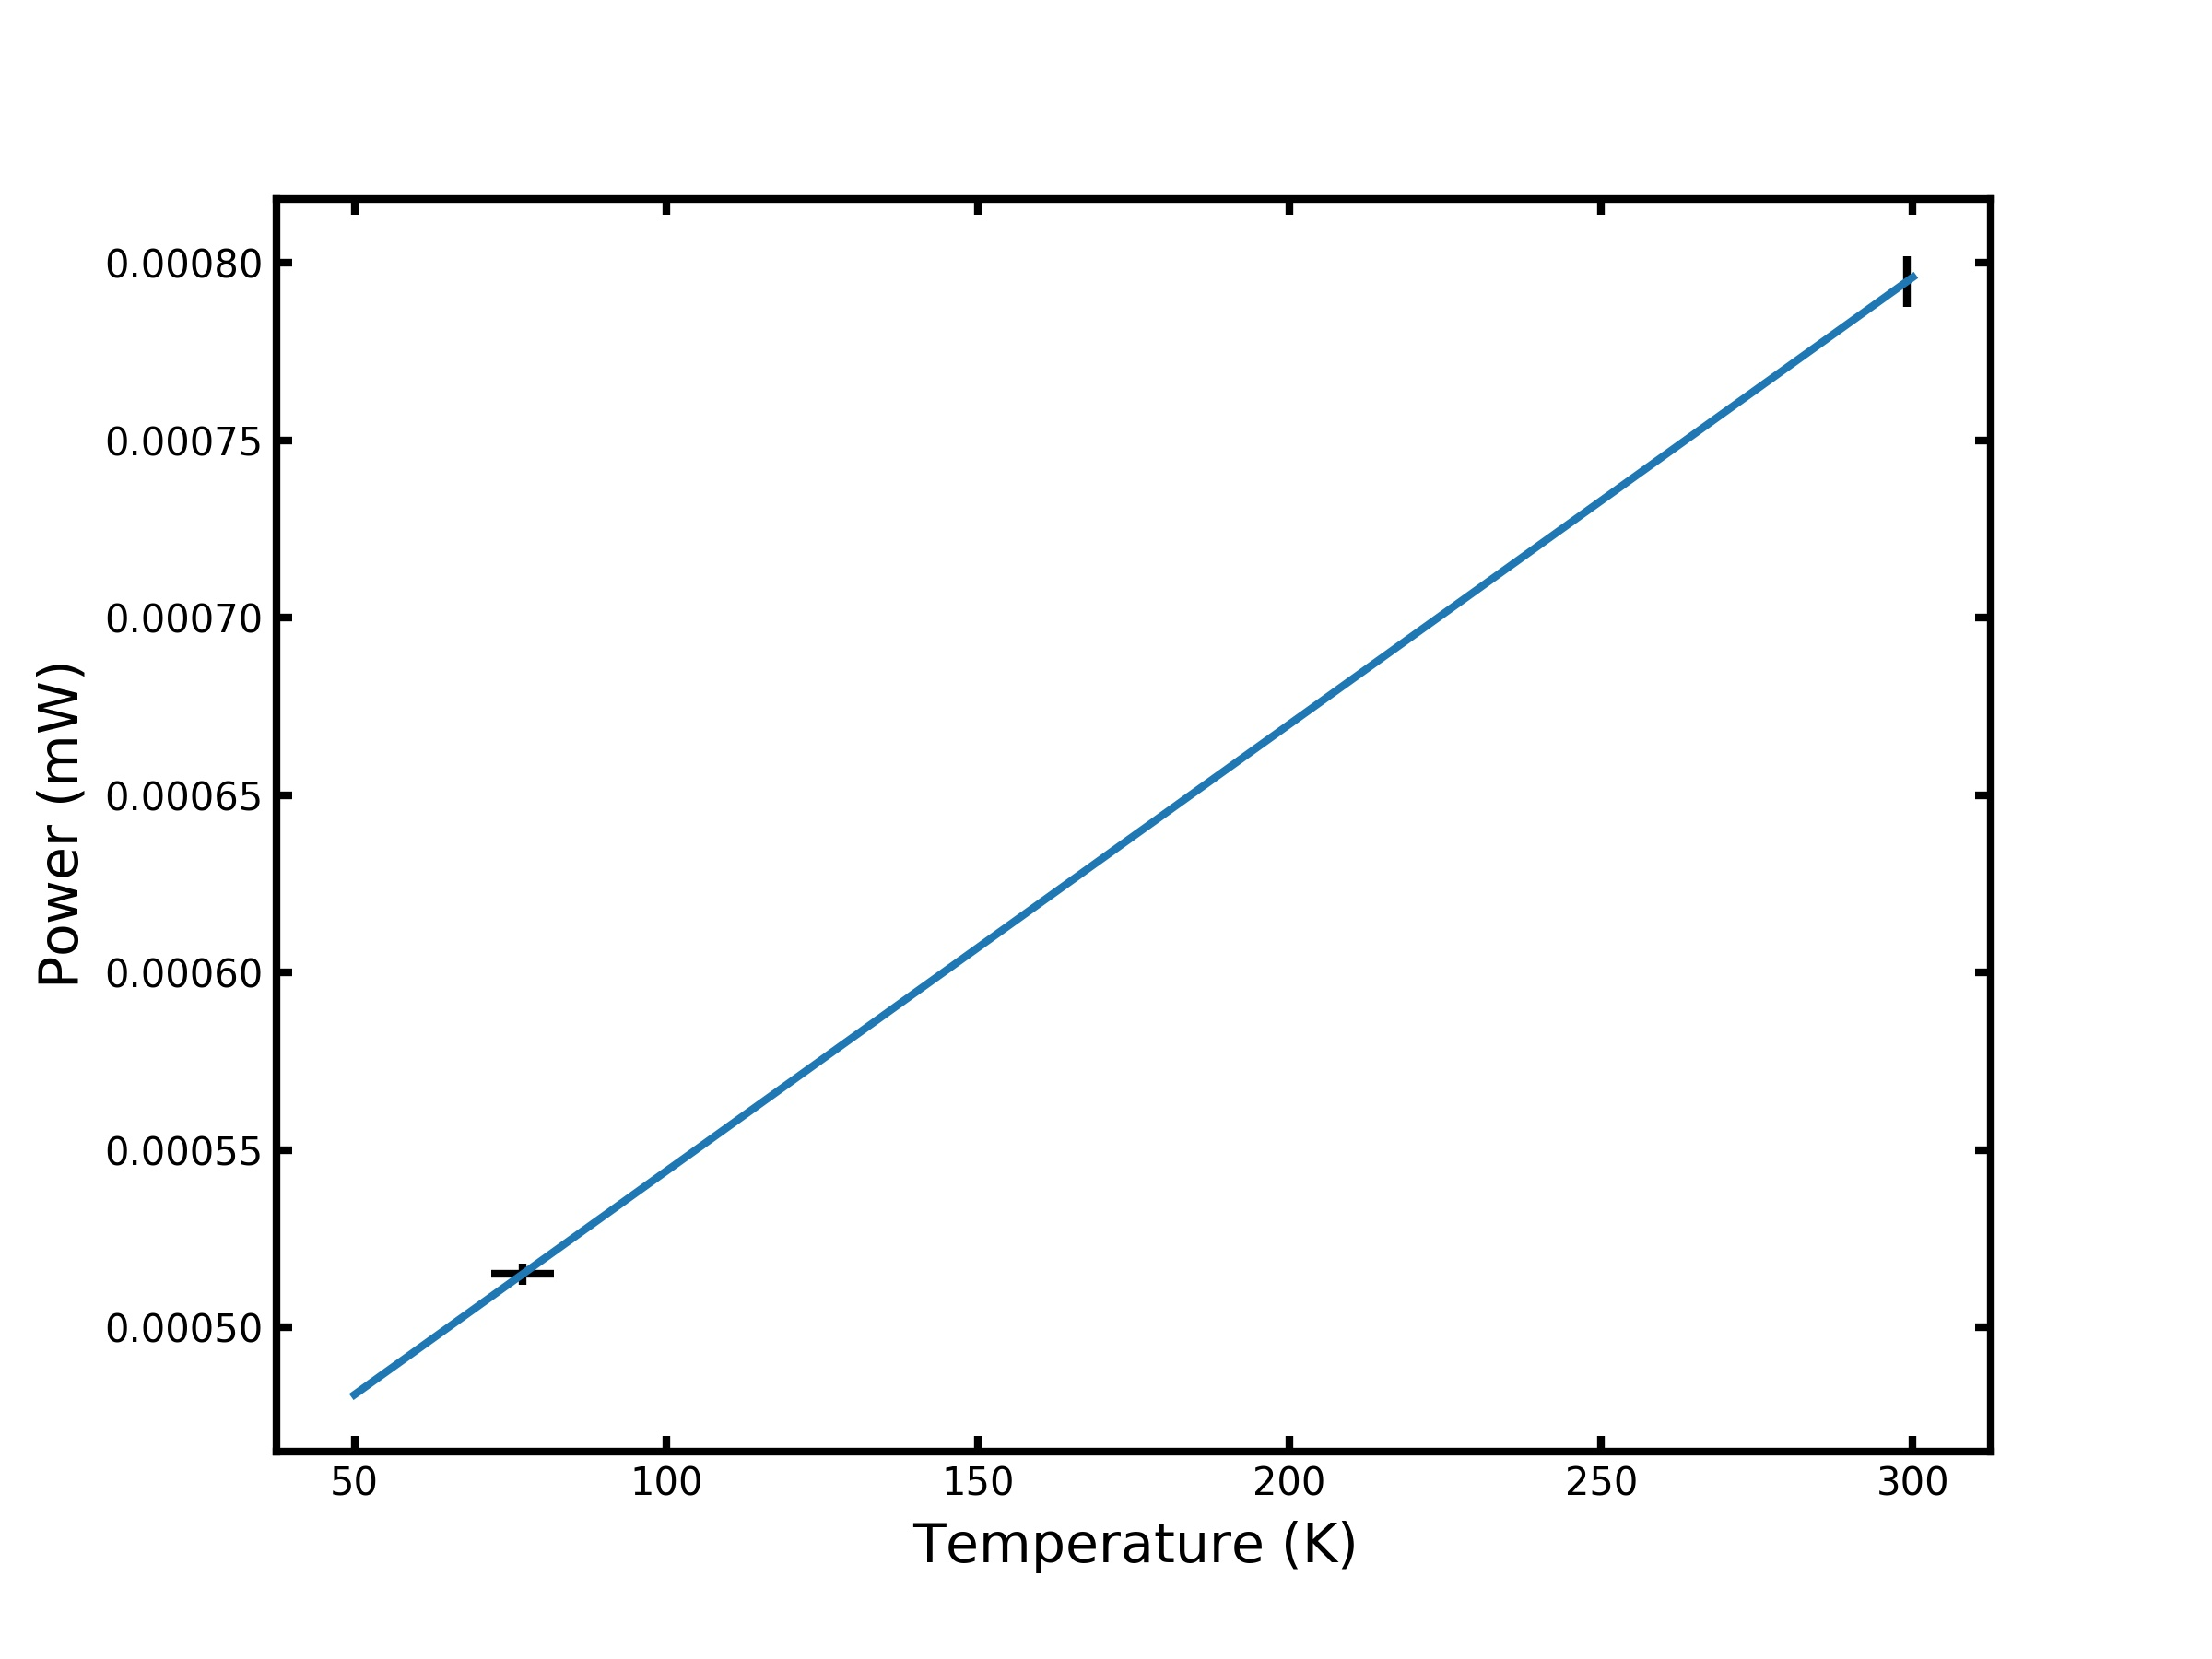
\includegraphics[scale=.5]{fig/Exercise_5_2.jpg}
\caption{Hot-Cold calibration of the superheterodyne receiver}
\label{fig1.52}
\end{figure}

With the function described in equation 5, we get a receiver temperature $T_{rec} = (332 \pm 13)$ K. This function will also be used for analysis in Exercise 1.6. 
We see that we get the same value of receiver temperature for the two methods used. Both methods are valid and use the same dataset. 

\subsection{Exercise 1.6}

We replace a resistor with a noise diode and measure its noise temperature using the calibration done in the previous exercise. Measurement is done for 12 seconds and the LO frequency is set to 1.45 GHz with a power amplitude of 0 dBm. Recording of data is done with the same software and the result is plotted in Figure \ref{fig1.61}.

We calculate the mean of data points and use the linear fitting function of equation 5, which we acquired from calibration to calculate the noise temperature of the diode for a given output power. As a result, we get $T_{noise} = (5.337 \times 10^{5}  \pm 3.963 \times 10^{4}) K$. Our results are shown in Figure \ref{fig1.62}. The noise temperature is very large compared to the receiver temperature, thus, it has to be reduced to increase the sensitivity of the receiver and improve the detection of signals. 

\begin{figure}[H]
    \centering
    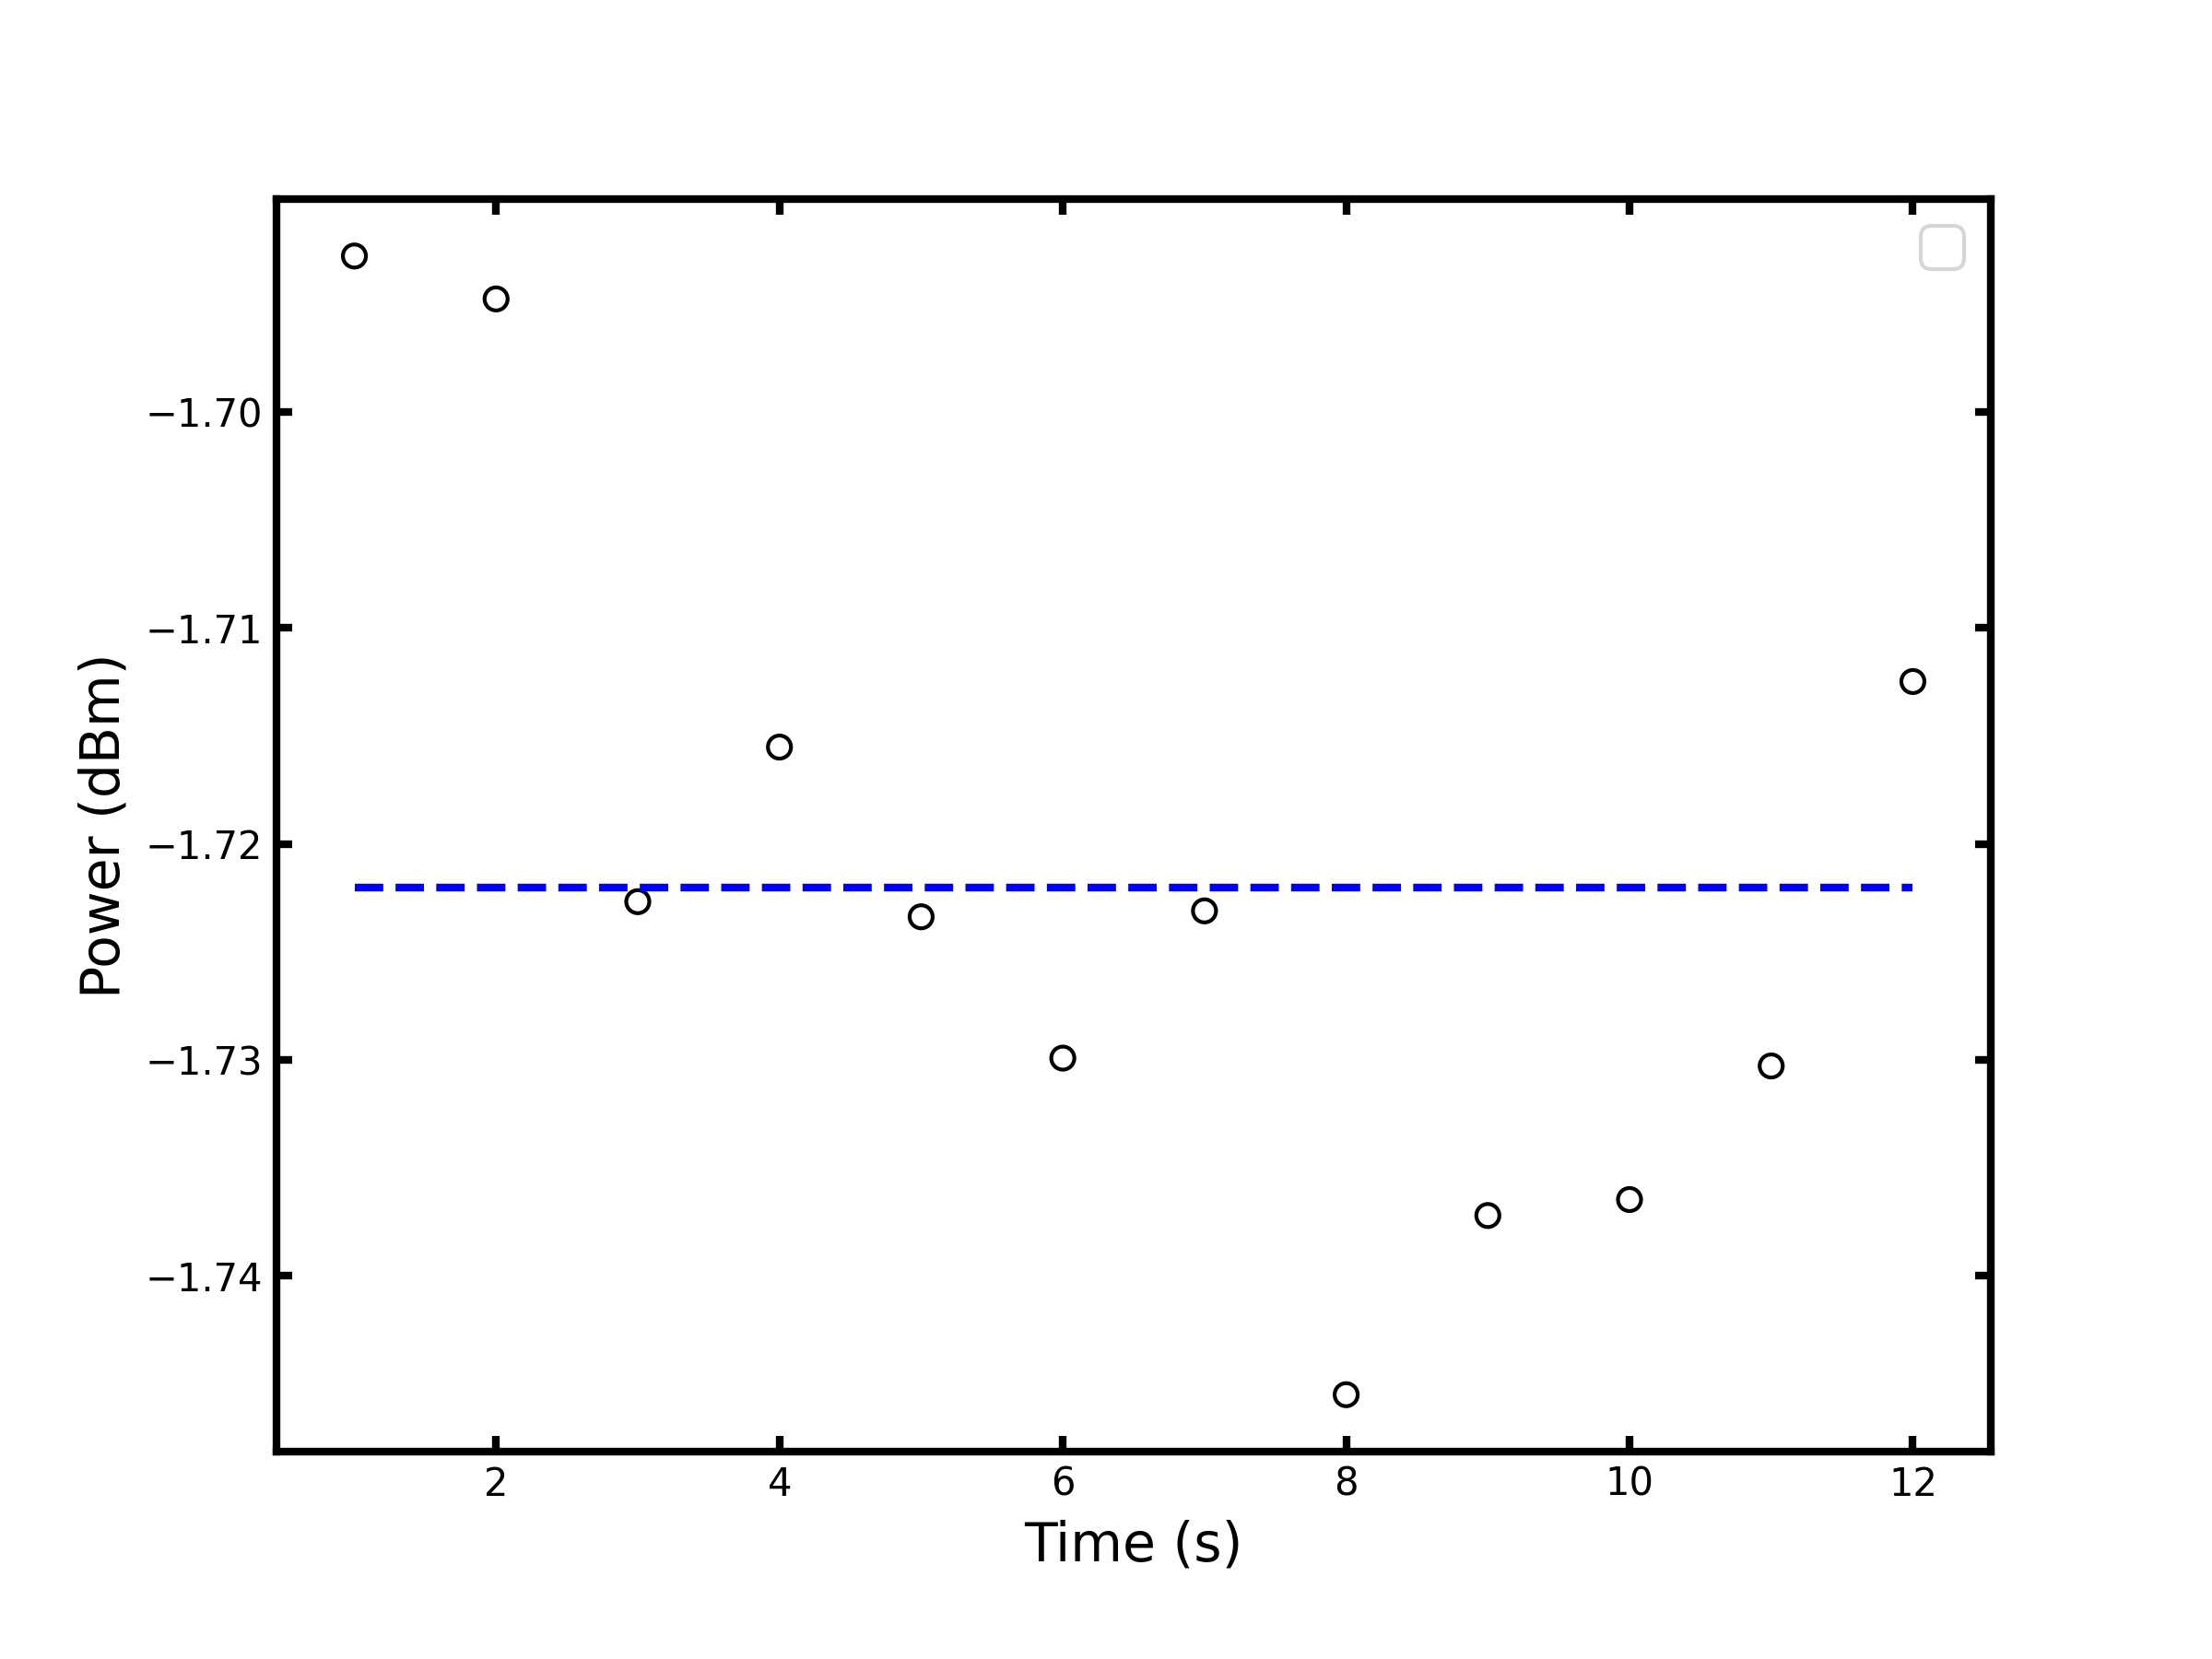
\includegraphics[scale=.5]{fig/Exercise_6_1.jpg}
    \caption{Diode noise power as a function of time}
    \label{fig1.61}
\end{figure}

\begin{figure}[H]
    \centering
    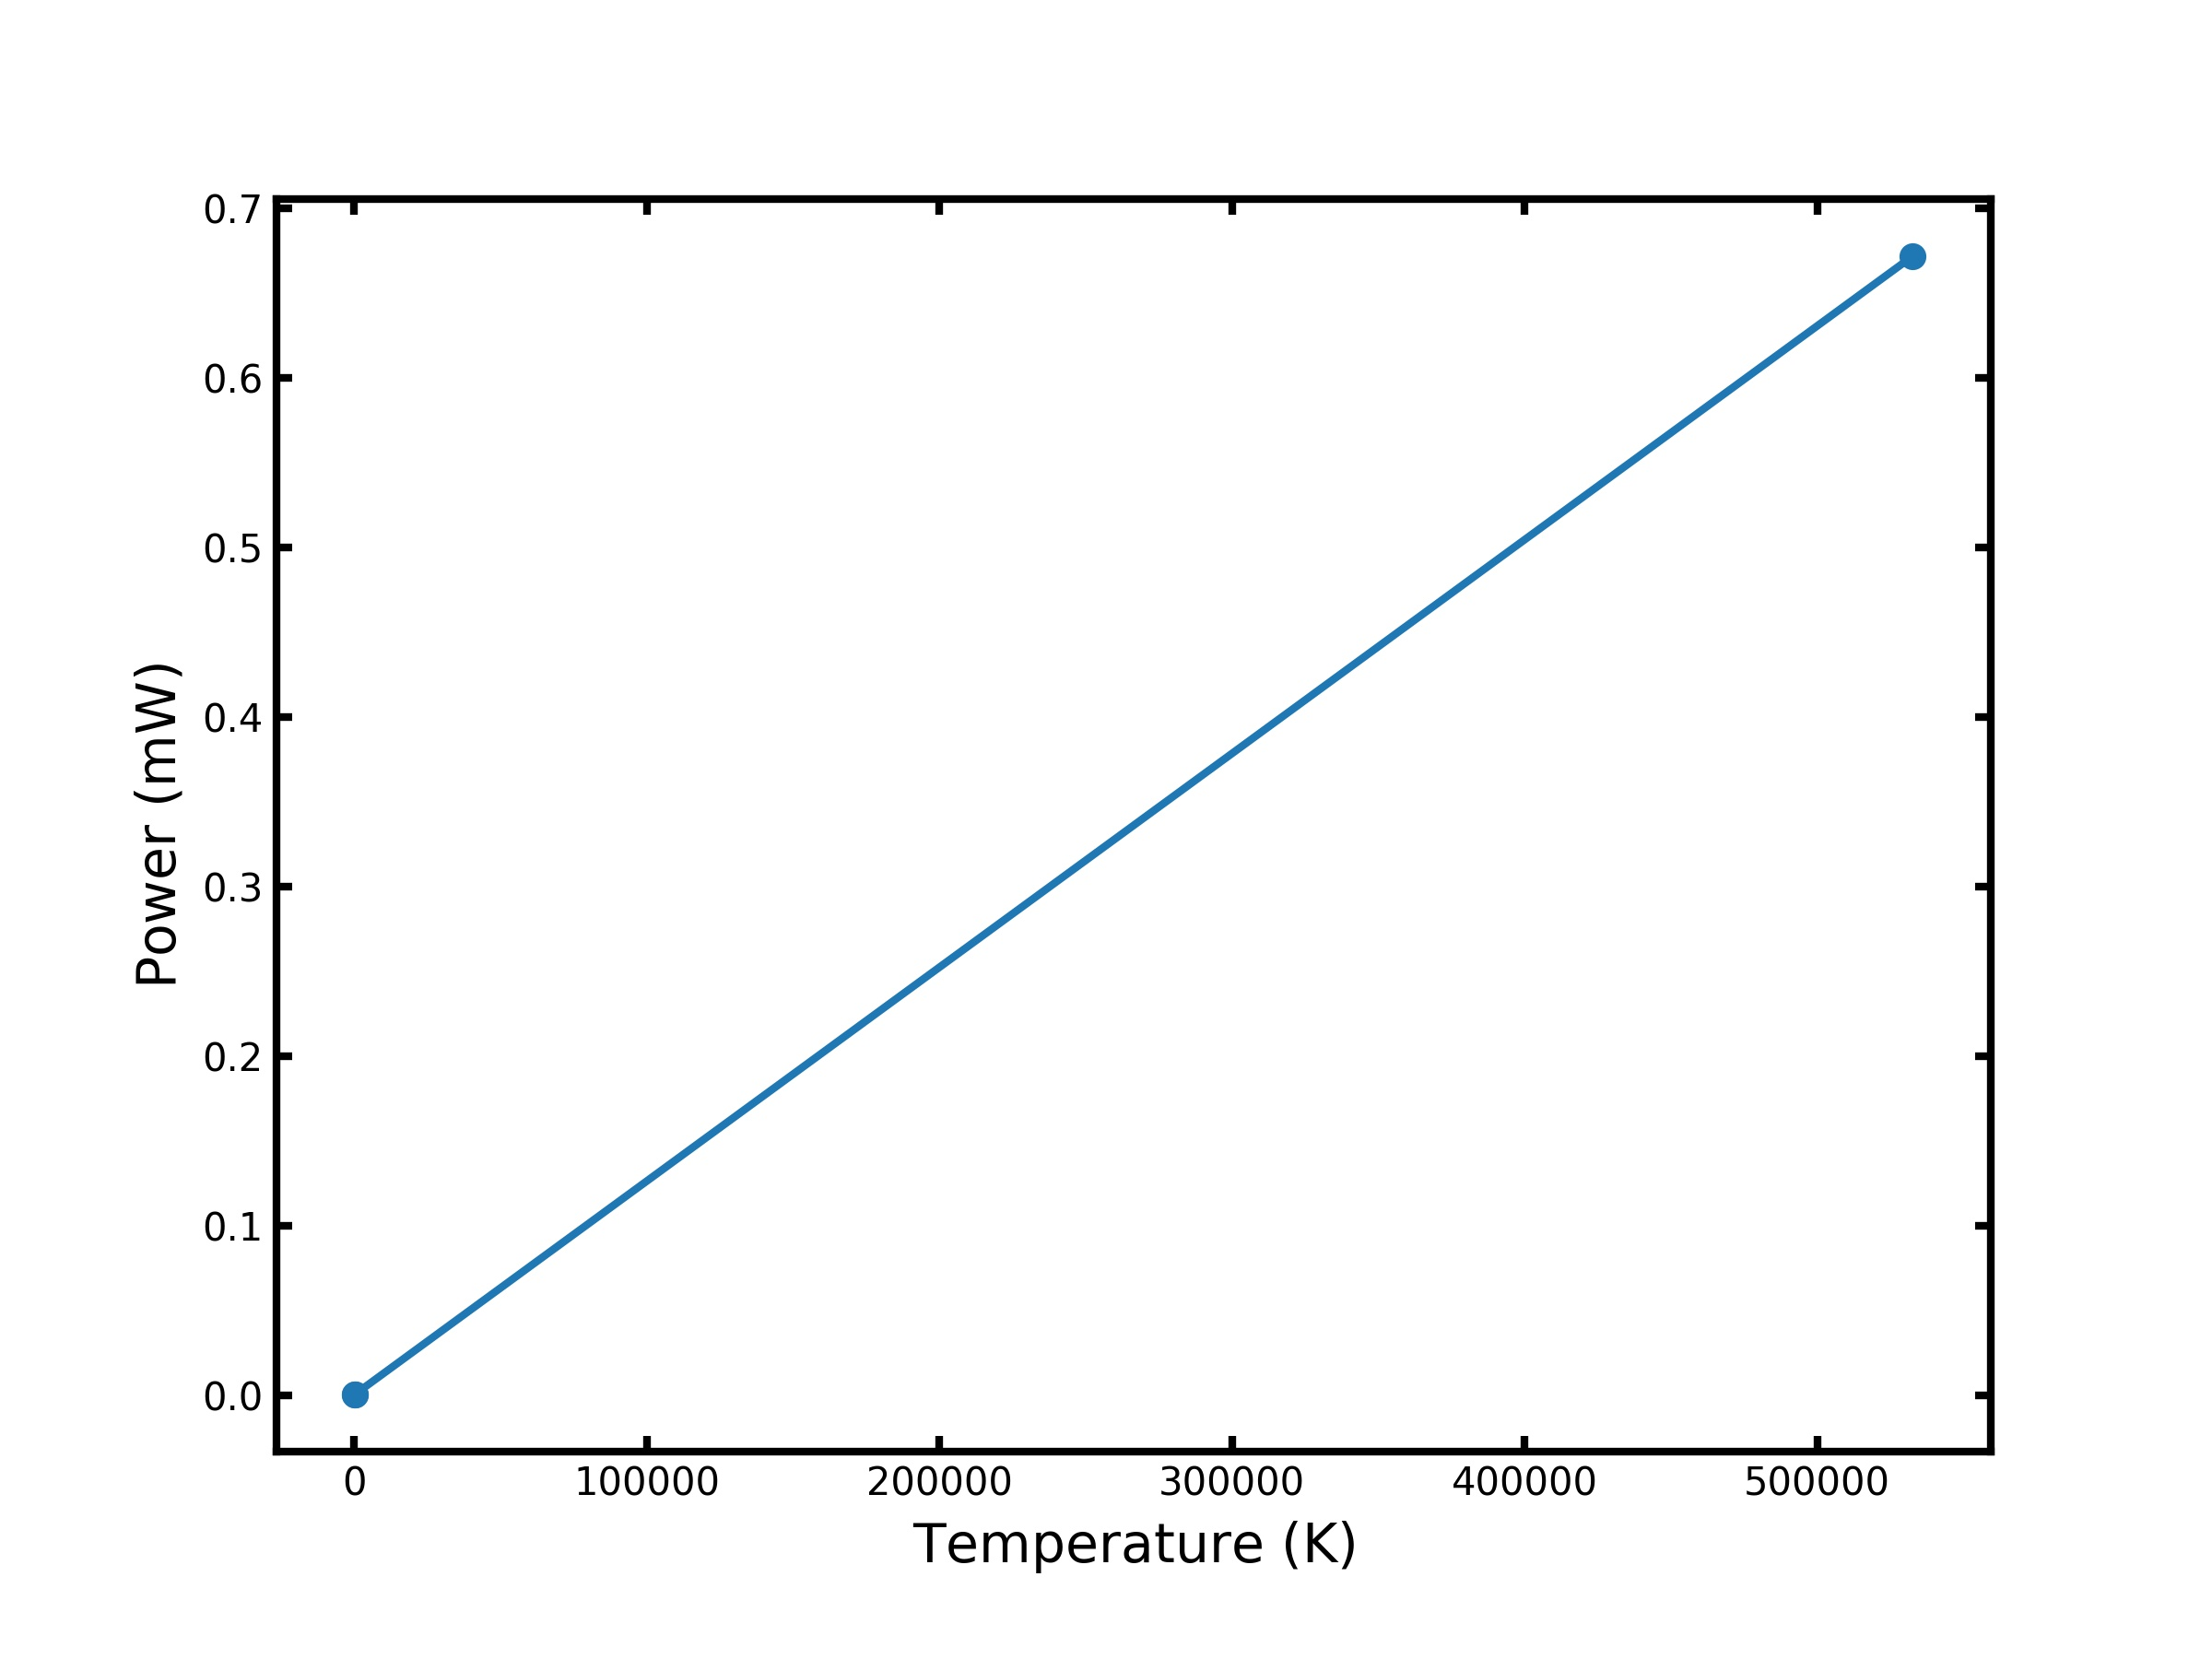
\includegraphics[scale=.5]{fig/Exercise_6_2.jpg}
    \caption{Determination of the noise temperature using the hot-cold calibration scale}
    \label{fig1.62}
\end{figure}

\subsection{Exercise 1.7}

Atmospheric absorption and emission play an important role in the determination of the antenna temperature as the atmosphere absorbs part of the signal and also emits its own radiation \cite{klein}. Thus, it has to be modeled and taken into account as modeling helps us understand how much of the signal is attenuated. In other words, from a received temperature, we can estimate the source temperature for a known attenuation model. The antenna temperature is described by the radiative transfer equation as follows \cite{klein}: 

\begin{equation}
\ T_{Antenna} = e^{-\tau} T_{B} + (1-e^{-\tau}) T_{atm}
\end{equation}

Where $T_{A}$ is the Antenna temperature, $T_{B}$ is the brightness temperature of the source, $T_{atm}$  is the atmospheric temperature, and $\tau$ is the optical depth. 


In this part of the experiment, we model the atmospheric attenuation using a variable attenuator. An attenuator is placed between the noise diode and the input of the superheterodyne receiver. The output power for varied attenuation values is recorded using the software by calling the function 'hotcold-power.py'. Then, average values of measurements of powers are calculated and plotted in Figure \ref{fig1.9} as a function of attenuation. 

\begin{figure}[H]
\centering
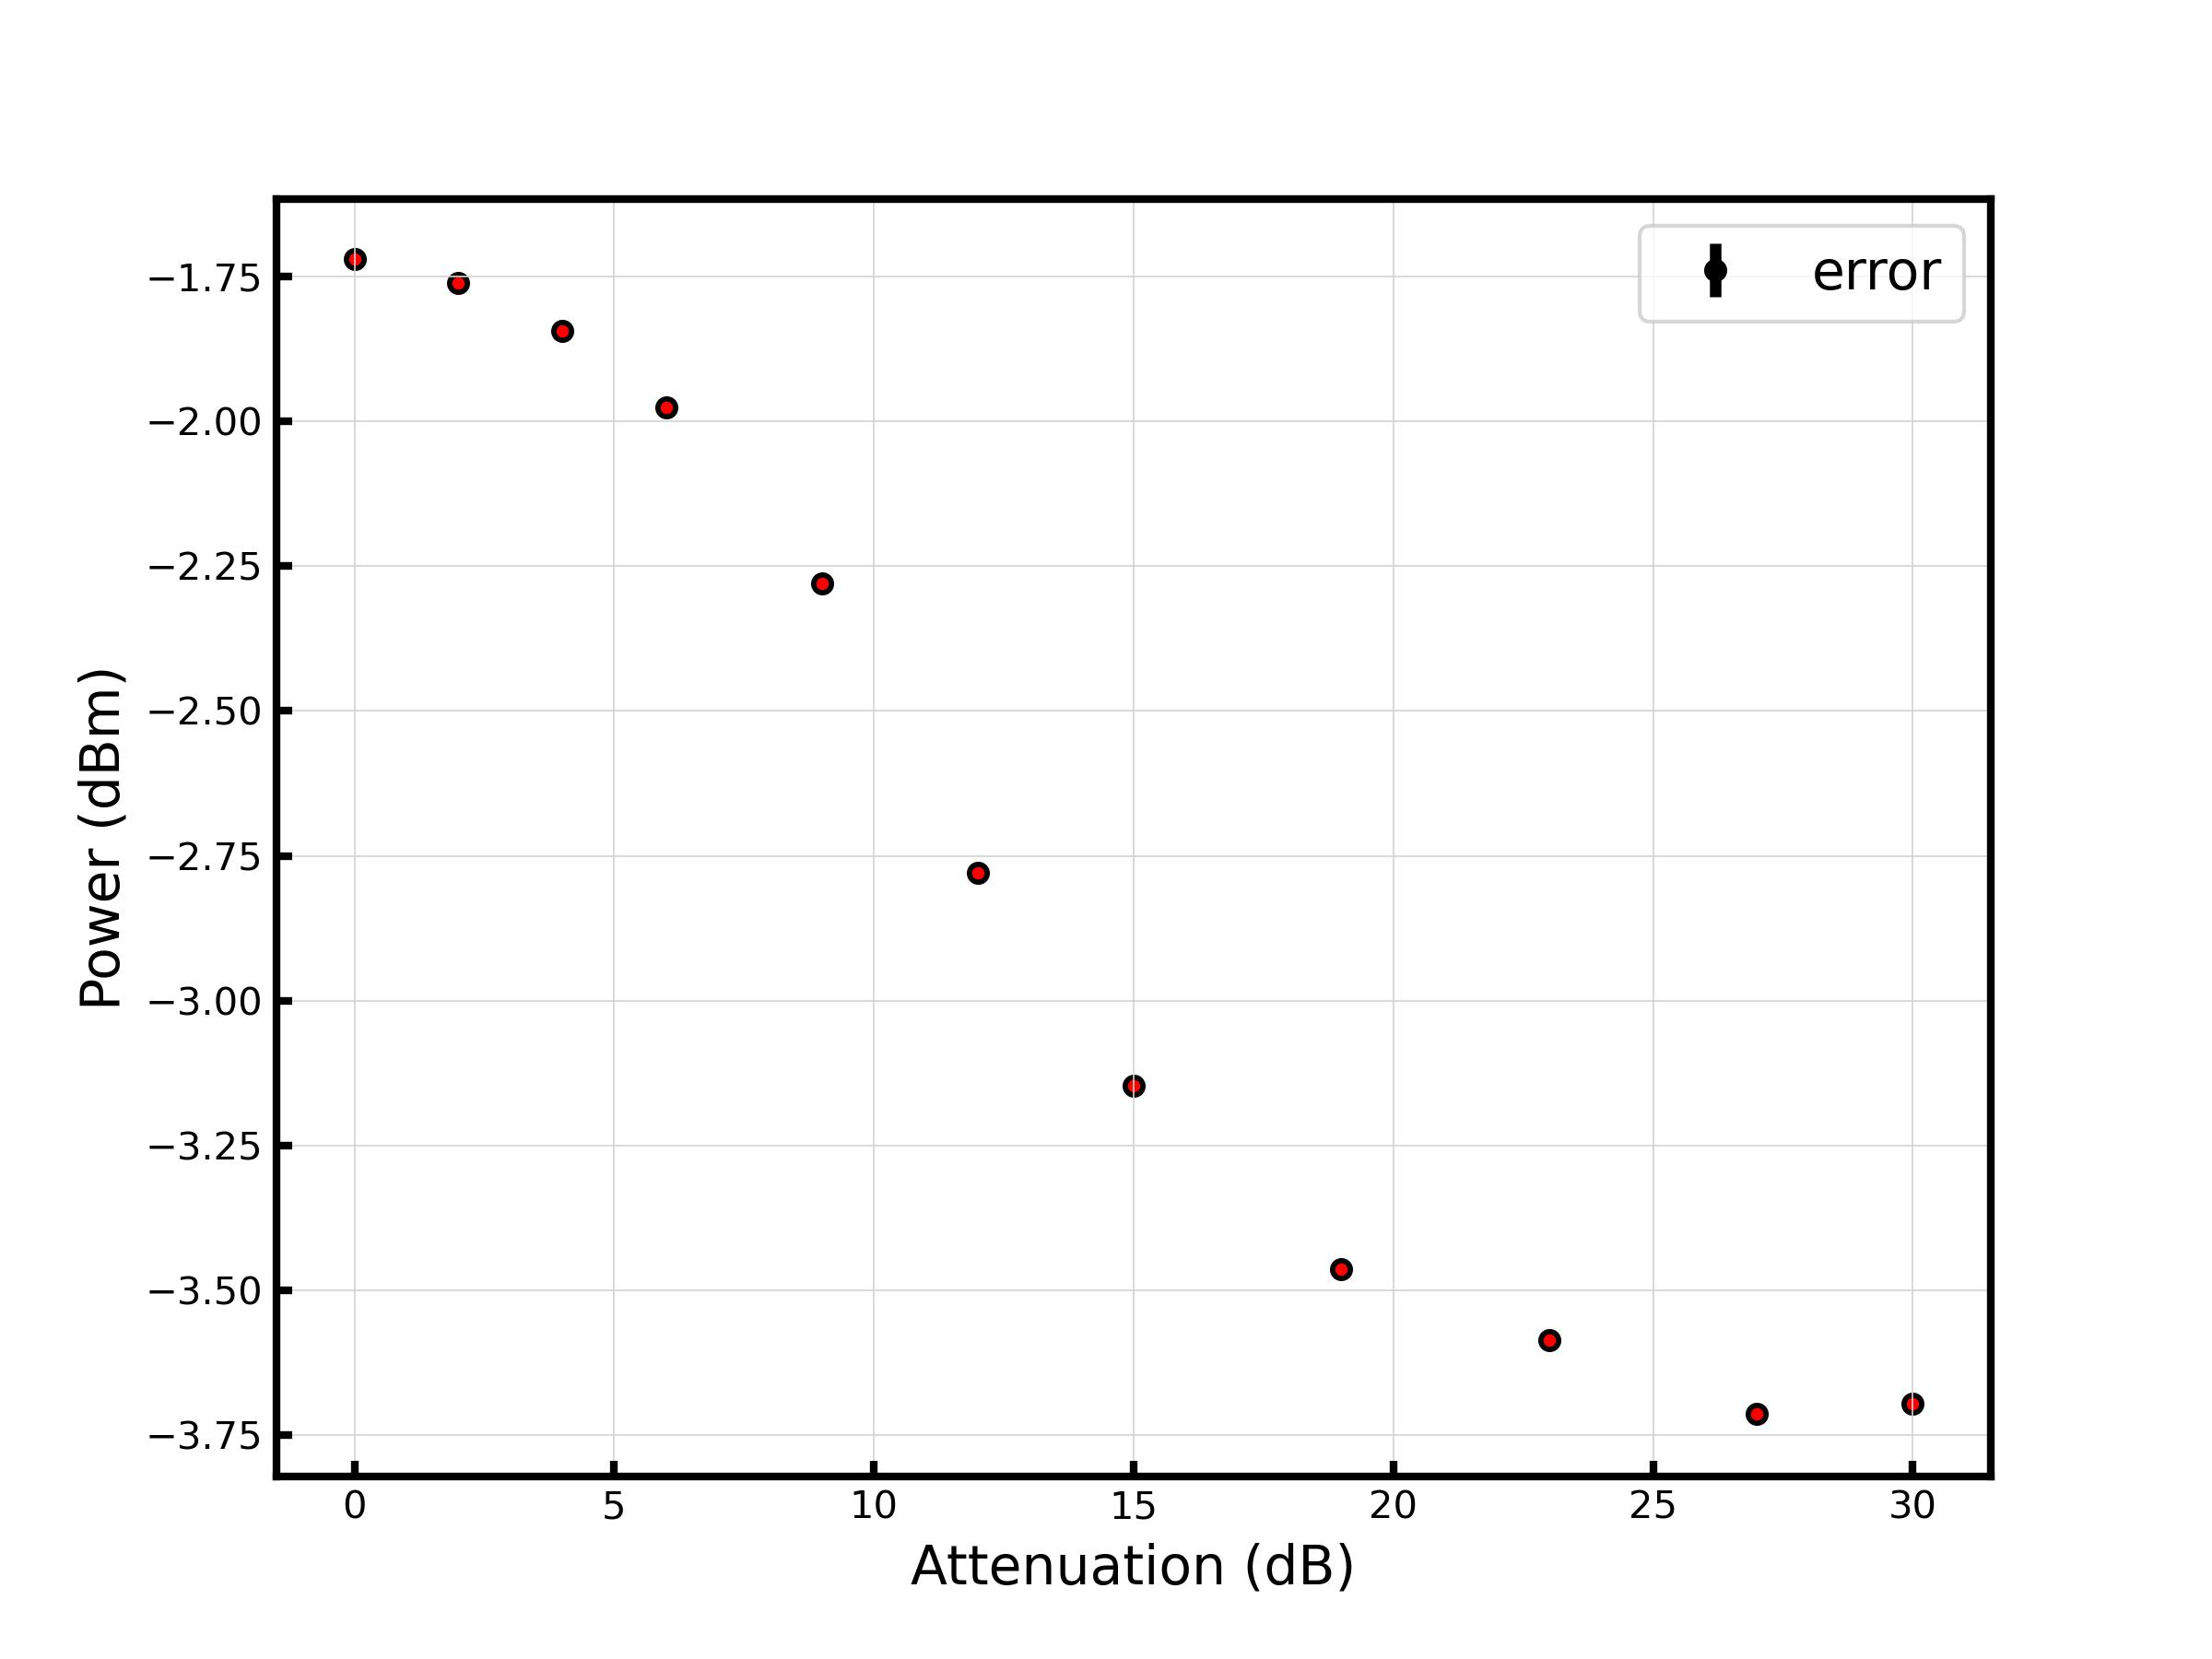
\includegraphics[scale=.5]{fig/Exercise 1.7.jpg}
\caption{Average power as a function of attenuation}
\label{fig1.9}
\end{figure}

As seen from the Figure \ref{fig1.9}, the exponential attenuation described in Equation 6 is demonstrated. For higher values of attenuation (or optical depth), less power from the signal source penetrates the atmosphere. 
For known values of atmospheric temperature, brightness temperature of the source, and optical depth, we can calculate the antenna temperature using equation 6 and also the system temperature for a known calibration factor. 

\subsection{Exercise 1.8}
In this exercise we move to do a radio spectroscopy. We replace the noise diode by an antenna and the signal generator acts as a radio source. The local oscillator is set to a frequency of 1.45 GHz (Continuous wave mode) and a power of amplitude of -10 dBm is given. The power is fed to the mixer and the output power of the mixer is fed to the frequency spectrum analyzer. 

A mixer produces an intermediate frequency given by \cite{klein}:

\begin{equation}
\ f_{IF} = f_{LO} - f_{RF}
\end{equation}

Where $f_{IF}$ is the intermediate frequency, $f_{LO}$ is the frequency of the local oscillator used, and $f_{RF}$ is the radio frequency generated by the signal generator. 
with an RF frequency of 1.6 GHz, we get an intermediate frequency of 150 MHz. 
As shown from Figure \ref{fig1.10}, what we see on the screen of the spectrum analyzer is nothing but the intermediate frequency because when tuning the frequency, no other harmonic frequencies were formed. This means that the mixer is efficiently producing the IF frequency after down-converting the RF signal. 

\begin{figure}[H]
\centering
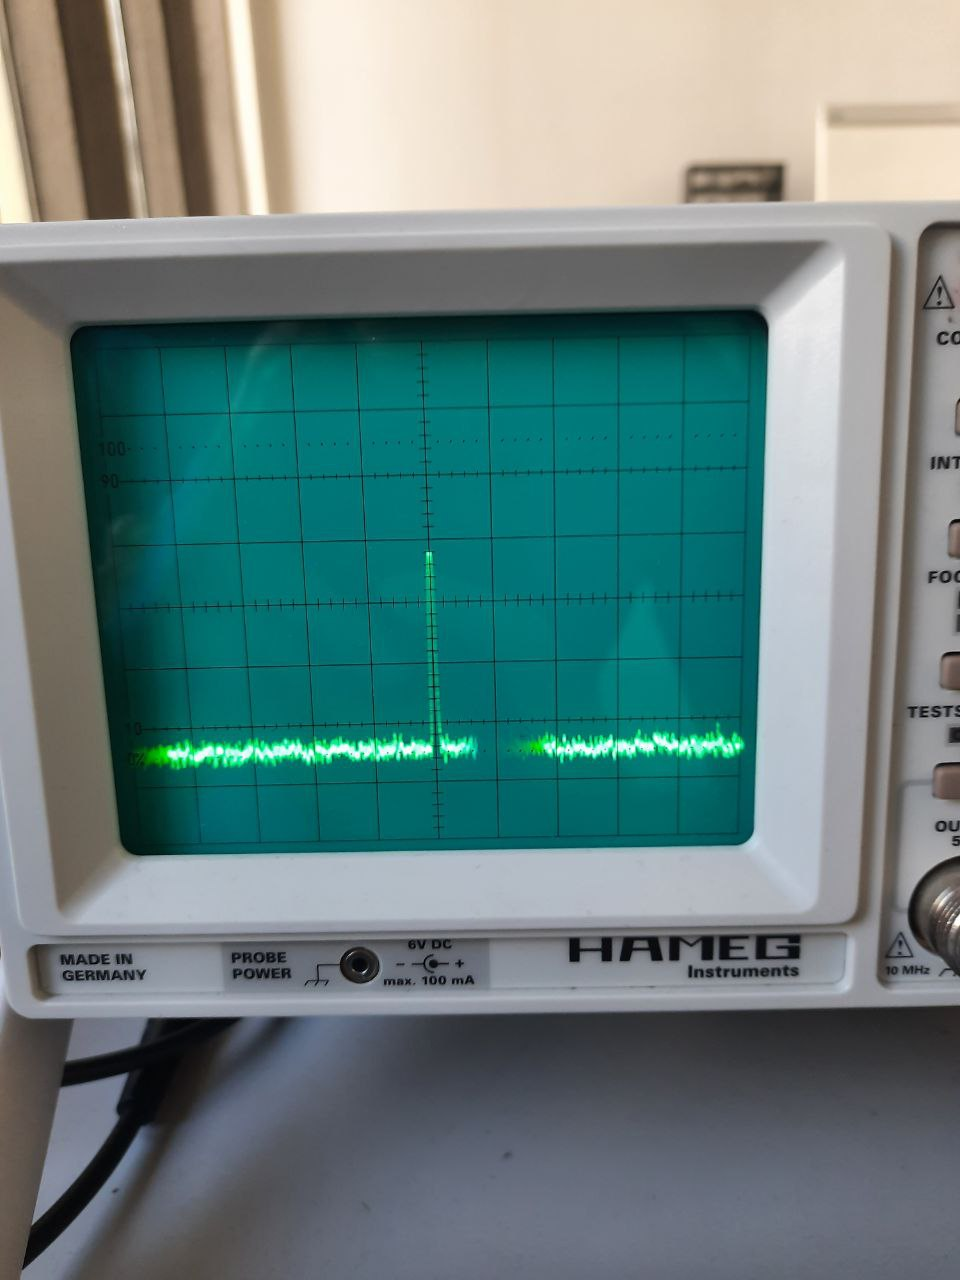
\includegraphics[scale=.2]{fig/Exercise 1.8.jpg}
\caption{Peak of spectral line at 150 MHz as seen from the frequency spectrum analyzer}
\label{fig1.10}
\end{figure}

\subsection{Exercise 1.9}
After we determined the receiver themperature and modeled the attenuation, now we investigate the effcent of measurement times on the sensitivity of the receiver. 
The receiver output is connected back to the SDR play receiver and the signal is recorderd for different length times (second to minutes). We first plot the average noise in dBm vs recording time in Figure \ref{fig1.11} and do a linear fitting. Then, we estimate the root mean square noise (rms) as a function of recording time and plot the results in Figure \ref{fig1.12}. The rms noise is estimated from the radiometer equation given by \cite{klein}:

\begin{equation}
\ \Delta T = \frac{T_{sys}}{\sqrt{\Delta \nu \cdot \tau}}
\end{equation}

Where $\Delta T$ is the sensitivity of the receiver or the rms noise in Kelvin, $T_{sys}$ is the system temperature which is approximated here to be equal to the receiver temperature for our calculations, $\Delta \nu$ is the bandwidth of the system (taken to be 2 MHz), and $\tau$ is the measurement time. 
As can be seen from Figure \ref{fig1.12}, the noise decreases for longer measurement times since $\Delta T$ $\propto$ $\frac{1}{\sqrt{\tau}}$. We fit a function of the form $y = \frac{a}{\sqrt{x}} + b$, shown in red in Figure \ref{fig1.12}, and we see that the fitting curve perfectly passes through the points. 

In this experiment, a frequency analyzer is used and spectrum of the different measurement times for an intermediate frequency of 150 MHz are recorded. On the frequency analyzer, we see a narrow sharp line presenting intermediate frequency, an example of a spectrum is shown in Figure \ref{fig1.13}. Also, we show in Figure \ref{fig1.14} the even distribution of peak in frequency scale upon zooming in the peak illustrated in Figure \ref{fig1.13}. We see multiple peaks separated by slightly less than 50 Hz. These peaks are probably produced by the mixer and are relatively weaker than the main peak.

Line intergrals of the different spectrums is performed using trapezoidal intergration with scipy library in Python \cite{scipy}. The results are shown in units of $W Hz^{-1} m^{-2}$ in Table \ref{T7}. 

Assuming that a line comes from a cloud in thermal equilibrium we can estimate the temperature of that source by considering the temperature to be the brightness temperature, which can be given in the radio regime by \cite{klein}:

\begin{equation}
\ T_{B} = \frac{I_{v} c^{2}}{2k_{B} \nu ^{2}}
\end{equation}

Here, $I_{v}$ is the intensity, or brightness which is the peak intensity for our analysis. $c$ is the speed of light, $k_{B}$ is Boltzman constant, and $\nu$ is the intermediate frequency (150 MHz). The resulting value of temperatures are also shown in Table \ref{T7}.

\begin{figure}[H]
\centering
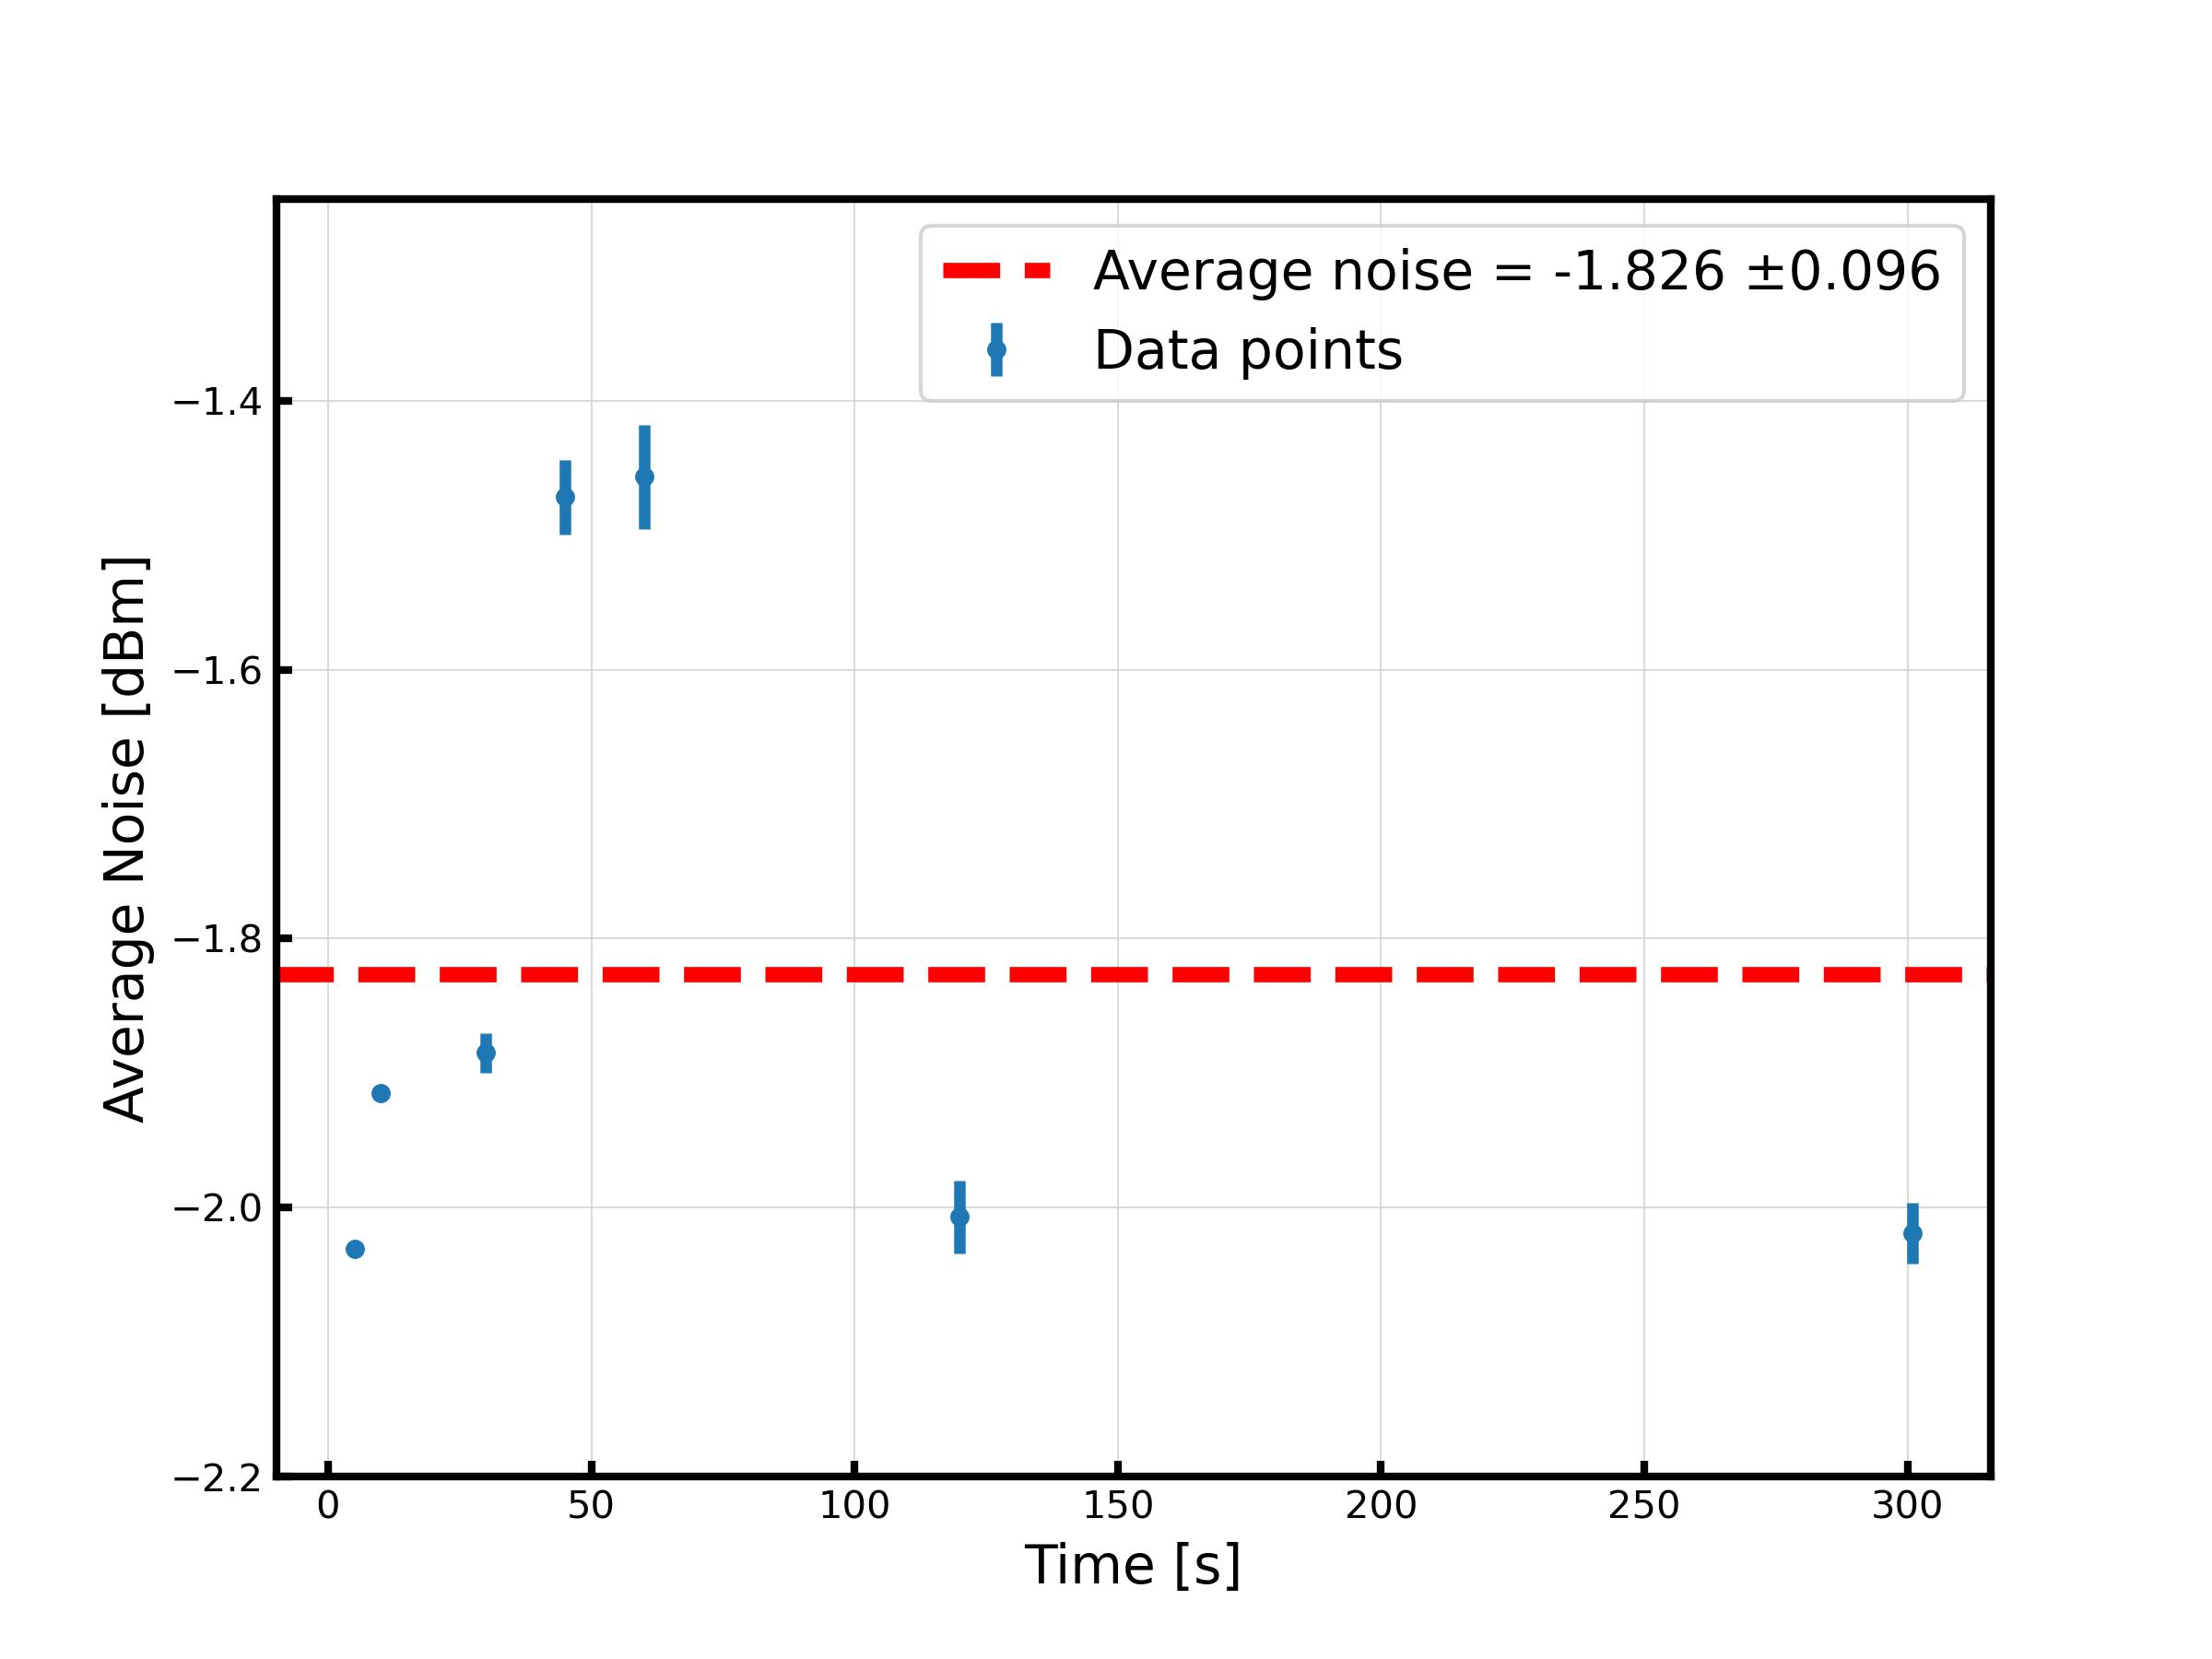
\includegraphics[scale=.5]{fig/Exercise 1.91.jpg}
\caption{Peak of spectral line at 150 MHz as seen from the frequency spectrum analyzer}
\label{fig1.11}
\end{figure}

\begin{figure}[H]
\centering
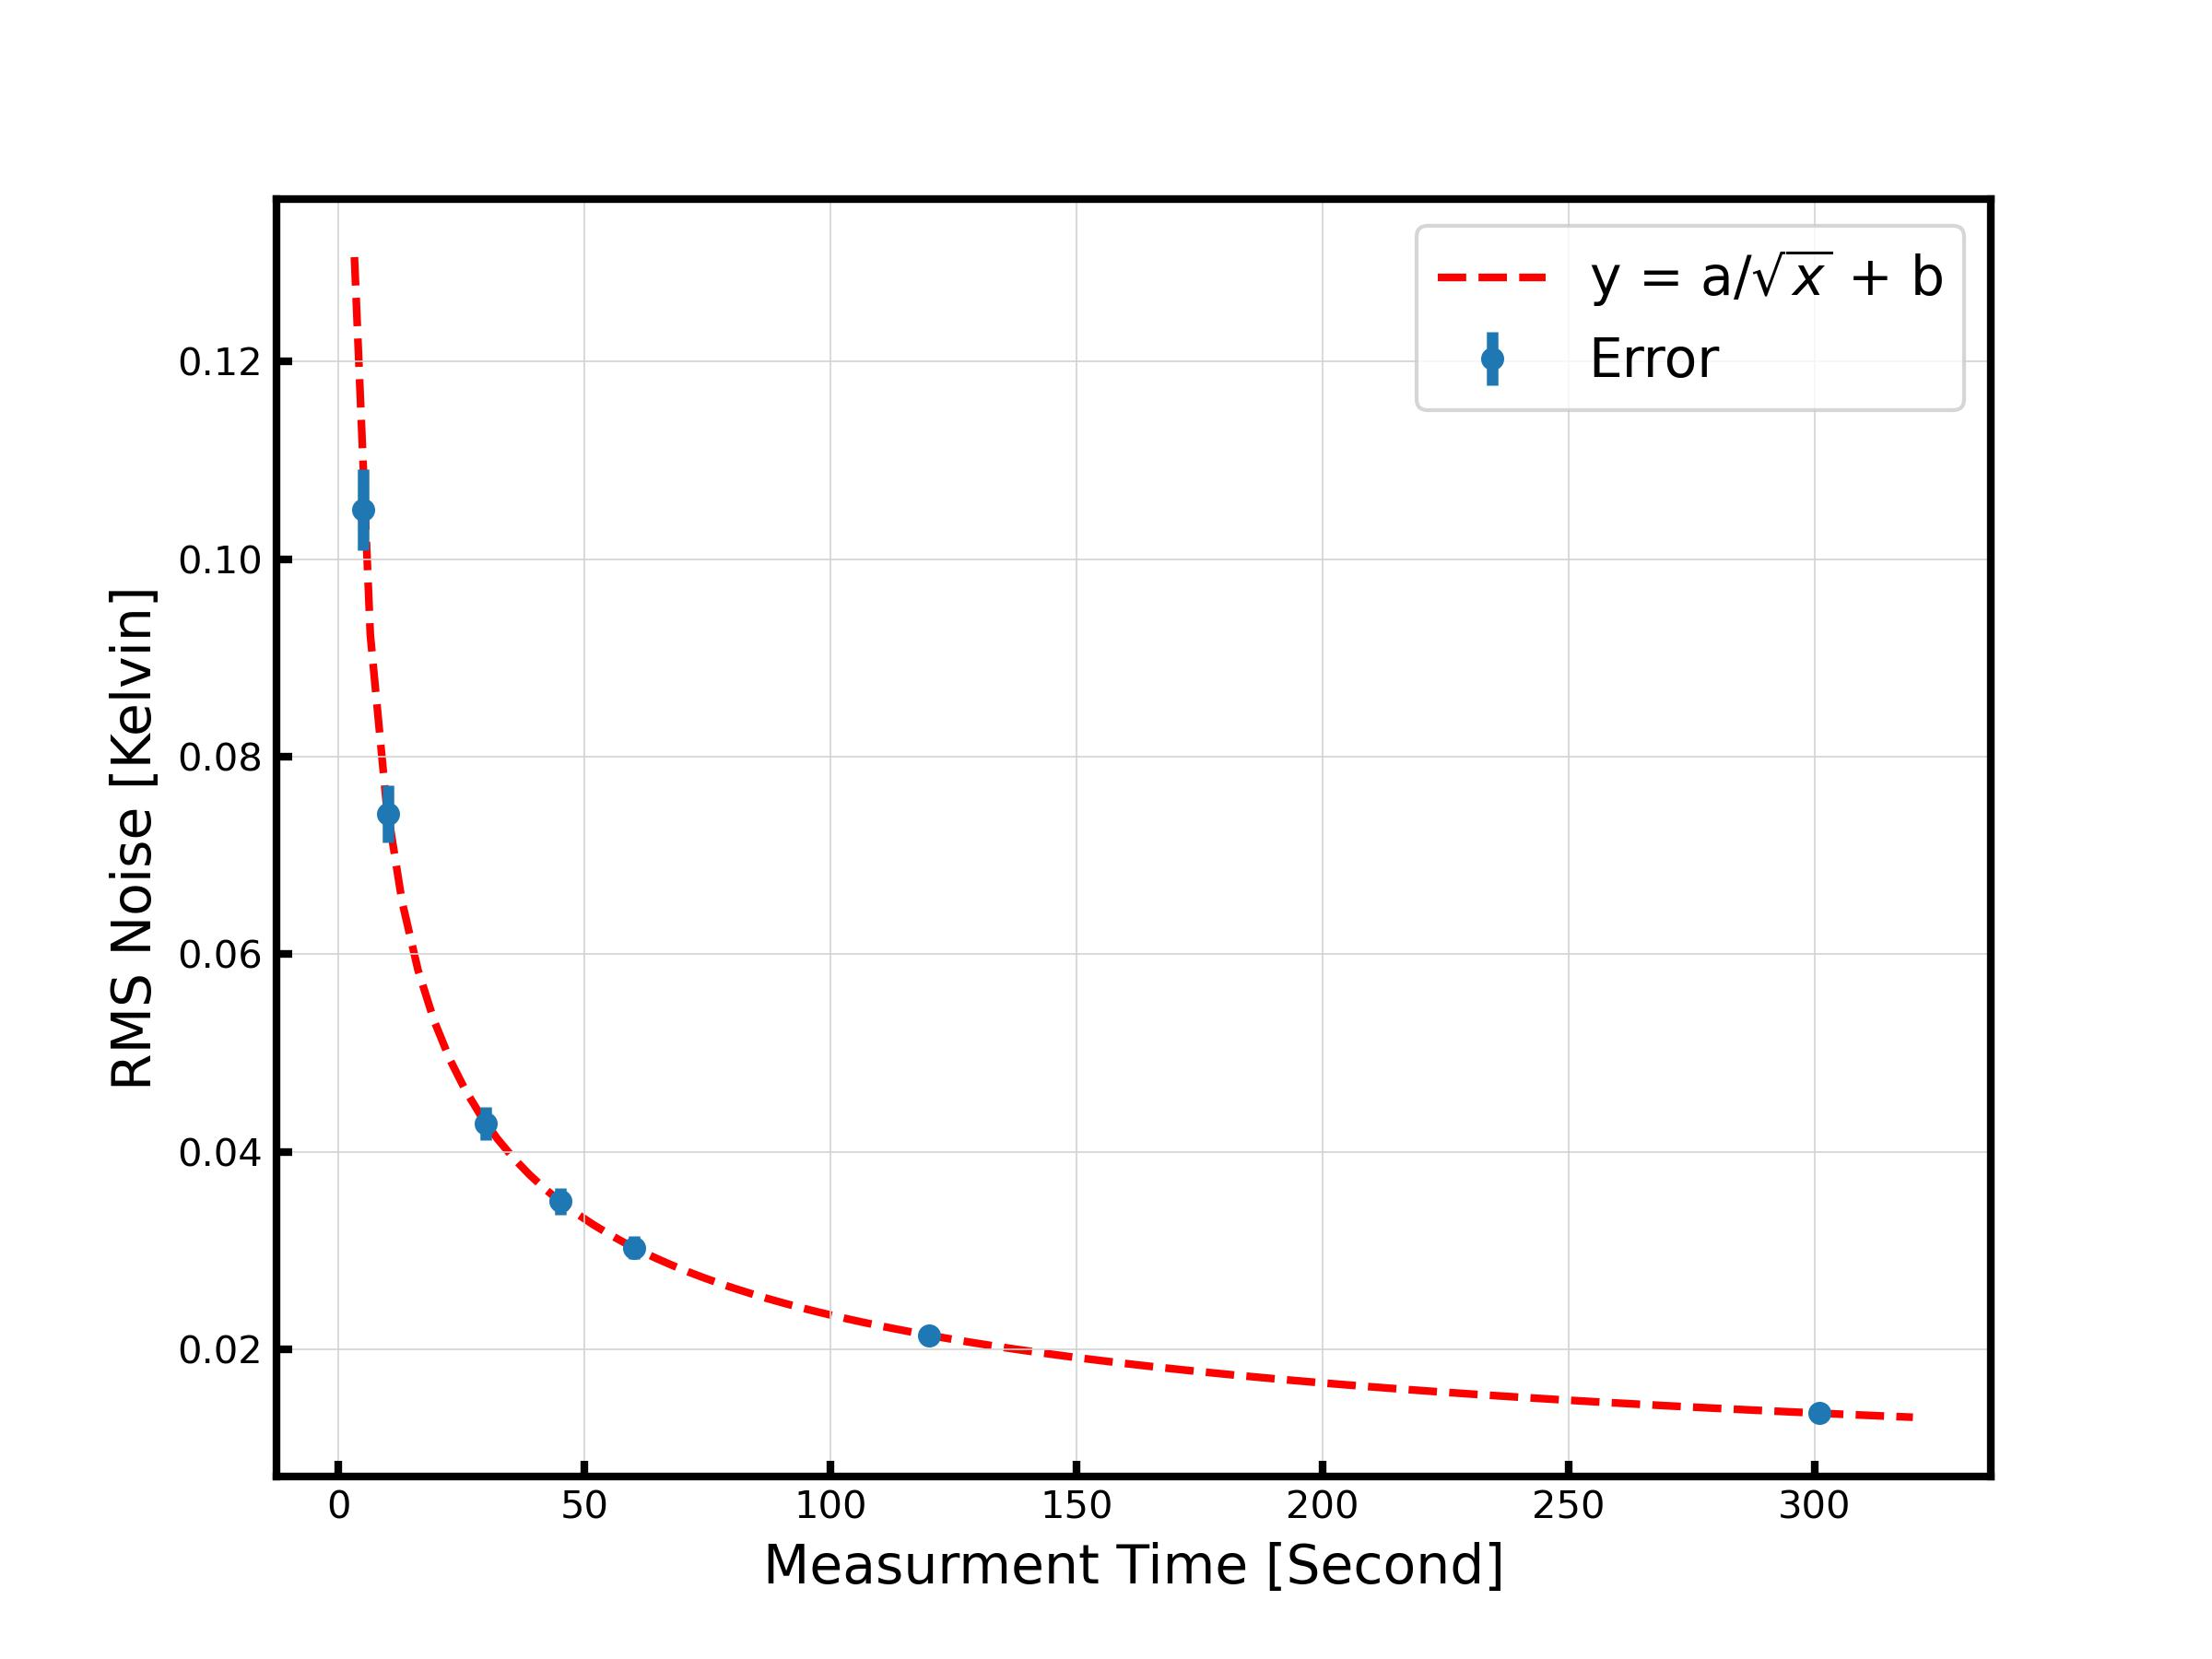
\includegraphics[scale=.5]{fig/Exercise 1.92.jpg}
\caption{Peak of spectral line at 150 MHz as seen from the frequency spectrum analyzer}
\label{fig1.12}
\end{figure}

\begin{figure}[H]
\centering
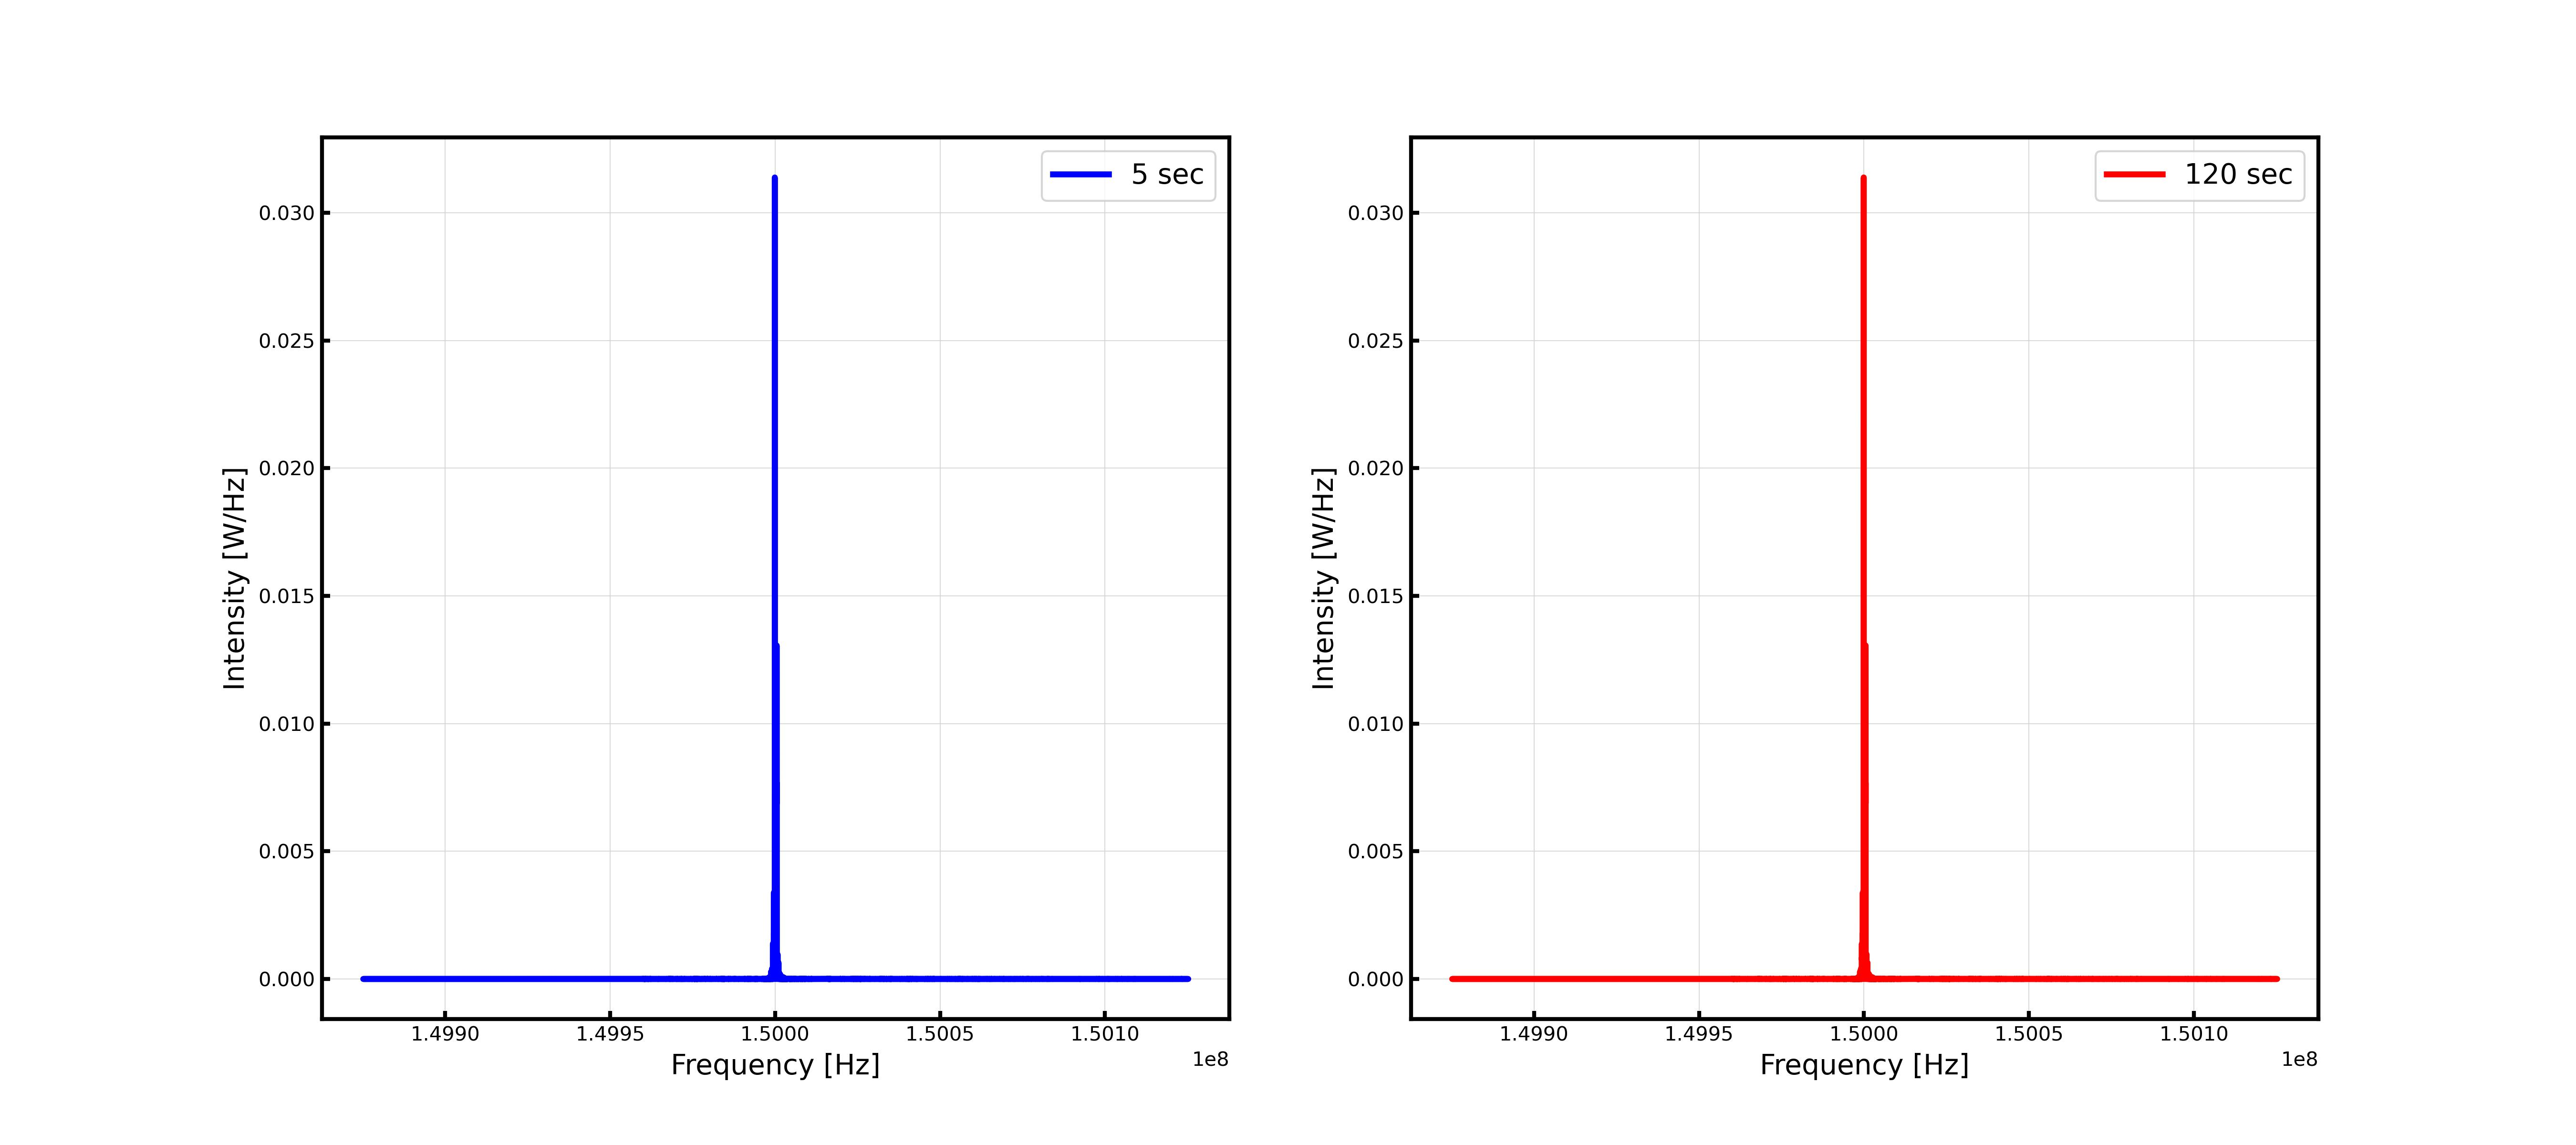
\includegraphics[scale=.3]{fig/Exercise 1.93.jpg}
\caption{Peak of spectral line at 150 MHz as seen from the frequency spectrum analyzer}
\label{fig1.13}
\end{figure}

\begin{figure}[H]
\centering
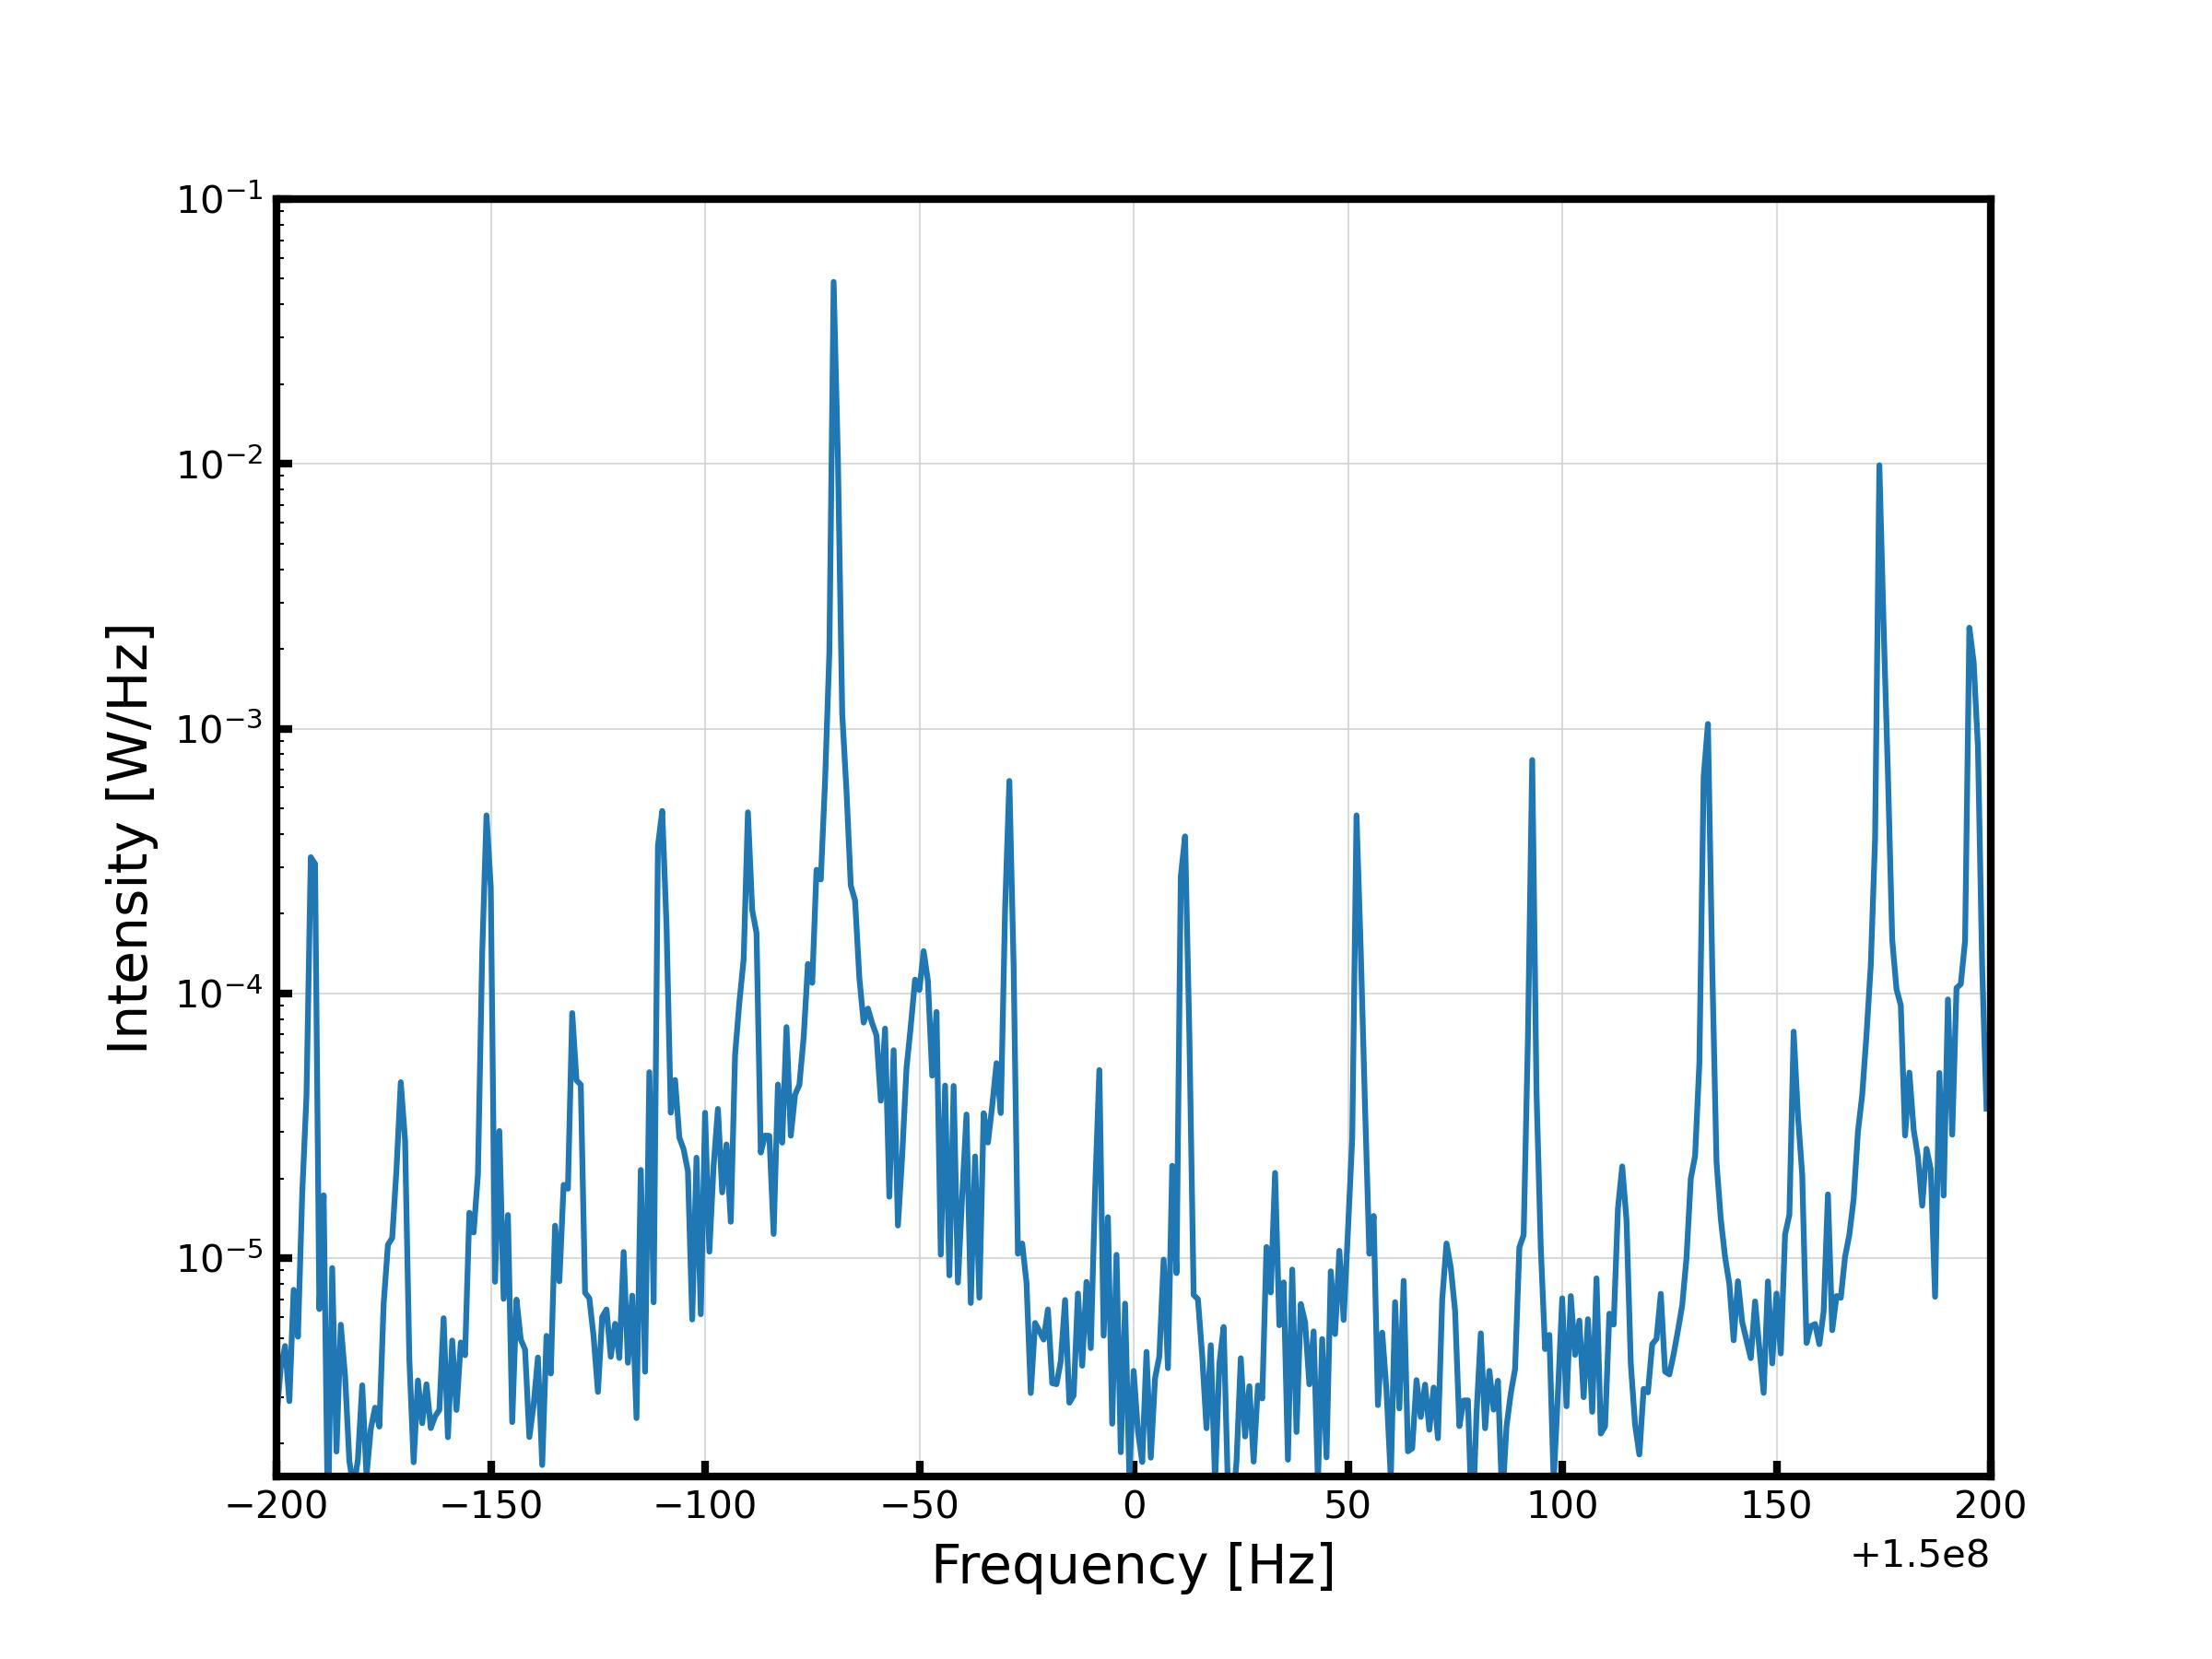
\includegraphics[scale=.5]{fig/Exercise 1.94.jpg}
\caption{Peak of spectral line at 150 MHz as seen from the frequency spectrum analyzer}
\label{fig1.14}
\end{figure}


\begin{table}[H]
    \centering
    \caption{Radio Spectroscopy Measurements}
    \label{T7}
    \begin{tabular}{c |c |c |c}
        \hline
        \hline
        Measurement Time& Peak Intensity & Integrated Flux & Brightness Temperature \\\relax
        [s] & [$\mathrm{W Hz^{-1} m^{-2}}$] & [$\mathrm{W m^{-2}}$]  & [K] \\
        \hline
        5 & 0.049 & 0.365 & $7.01 \times 10^{21}$ \\
        10 & 0.024 & 0.379 & $3.43 \times 10^{21}$ \\
        30 & 0.031 & 0.344 & $4.51 \times 10^{21}$ \\
        45 & 0.017 & 0.523 & $2.47 \times 10^{21}$ \\
        60 & 0.012 & 0.428 & $1.70 \times 10^{21}$ \\
        120 & 0.031 & 0.574 & $4.52 \times 10^{21}$ \\
        300 & 0.010 & 0.498 & $1.41 \times 10^{21}$ \\
        \hline
    \end{tabular}
    \label{tab:mytable}
\end{table}

\subsection{Exercise 1.10}
The most common type of antennas used in FM stations is the quarter-wave whip antenna which is roughly one quarter of the length of a radio wave in the radio band \cite{antennas}. Thus, for for efficient transmission at a frequency of 100 MHz, the ideal antenna length would be: 

\begin{equation}
\ L_{antenna} = \frac{\lambda}{4} = \frac{c}{4f} = 0.75 m
\end{equation}

 \section{Setting up a twin radio interferometer}
 In the second part of our lab, we set up a phased-switched radio interferometer using two dished on the roof of the Argelander Institute for Astronomy (AIFA). We first discuss the parameters that affect the resolution of the interferometer, investigate the source of emission from the sun. Then, we do scaning of the sun to get the fringe pattern and do analysis to calculate its diameter.
 
 \subsection{Exercise 2.1}
 In general, a radio telescope consist of a radio receiver which is studied in the section \ref{S1} and a parabolic radio antenna. The resolution of a single dish is given by the following equation\parencite{lecturenote}:
 \begin{equation}
 \label{eq2.1}
 \theta = 1.22 \dfrac{\lambda}{D}
 \end{equation}
 $\theta$ is the resolution, $\lambda$ is the observing wavelength and $D$ is the diameter of the antenna. However, the resolution for a twin dish is\parencite{lecturenote} :
  \begin{equation}
 \label{eq2.2}
 \theta = 1.22 \dfrac{\lambda}{B}
 \end{equation}
 where $B$ here is the distance between two antennas. This indicates that when considering the same angular resolution, a larger parabolic surface results in a longer operational wavelength, and the opposite is true for a smaller parabolic surface. So, if the distance between two dishes(baseline) in the twin interferometer telescope or the diameter of the dish in a single antenna is increased the resolution of the antenna according to equation \ref{eq2.1} and \ref{eq2.2} increases. In fact, the telescope's ability to achieve angular resolution and image quality is constrained by various factors. One such factor is the antenna's efficiency, which pertains to the precision of the reflecting surface. Even minor deviations from an entirely perfect parabolic surface can have a considerable effect. 

 Additionally, the sensitivity of the radio receiver, which relies on the observed band width, also has an effect that can be explained using the radiometer equation\parencite{radiometereq}:
 \begin{equation}
 \label{eq2.3}
 \Delta T = \dfrac{T_{sys}}{\sqrt{\Delta\nu \tau}}
 \end{equation}
 where $\Delta T$ is the uncertainity in the noise temperature, $T_{sys}$ is the system temperature, $\Delta \nu$ is the band width and $\tau$ is the integration time. Furthermore, external factors like human-generated radio interference (FM), wind forces, temperature-induced distortions, and shifts caused by alterations in gravitational forces can obscure the signal\parencite{Tools}.


 \subsection{Exercise 2.2}
 According to the equation \ref{eq2.1}, The size of the parabolic surface directly influences the operational wavelength. As mentioned in the previous part, when considering the same angular resolution, a larger parabolic surface results in a longer operational wavelength, and the opposite is true for a smaller parabolic surface.

 \subsection{Exercise 2.3}

 \begin{figure}[H]
 \centering
 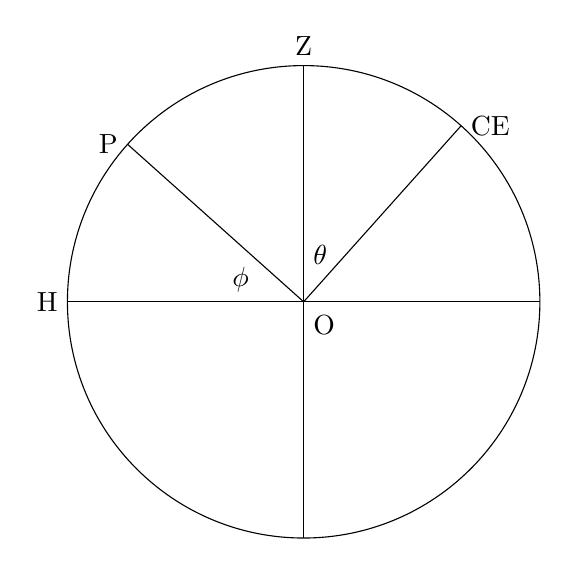
\begin{tikzpicture}
 \draw (2,2) circle (3cm); \node[below, right] at (2,1.7) {O};
 \draw (2,5) -- (2,-1); \node[above] at (2,5) {Z};
 \draw (5,2) -- (-1,2); \node[left] at (-1,2) {H};
 \draw (2,2) --(4,4.2360); \node[above,right] at (4,4.2360) {CE}; 
 \draw (2,2) --(-0.2360,4); \node[above,left] at (-0.2360,4) {P};
 \node[above] at (1.2,2) {$\phi$};
 \node[right] at (2,2.6) {$\theta$};
 \end{tikzpicture}
 \caption{Schematic of the equatorial system}
 \label{fig2.1}
 \end{figure}

 According to the figure \ref{fig2.1}, $O$ is the position of observer, $Z$ is the zenith point $P$ is the North Celestial Pole $CE$ is the celestial equator and $H$ is the horizon. The key point in this figure is that zenith point and horizon are orthogonal to each other and also North celestial pole and celestial equator are at right angles to each other.

 Latitude of the observer is the angel between zenith point and celestial equator($\theta$) and altitude of the north celestial pole is its angel with the horizon($\phi$).

 \begin{align}
 &\angle POZ = 90 - \phi  \qquad \angle POZ = 90- \theta \\
 &\Rightarrow 90 - \phi = 90 - \theta \Rightarrow \phi = \theta
 \end{align}

 \subsection{Exercise 2.4}

 Polaris is around 1 degree from the pole\parencite{lecturenote}. So the circumference of the polarise in minutes is $2\pi \time 60^\prime = 376.99^\prime$. The number of moons which could be fitted in this distance can be calculated by $\dfrac{376.99}{30} = 12.56$.   

 \subsection{Exercise 2.5}

 The sun atmosphere consist of 3 main layers\parencite{Thesun}:
 \begin{itemize}
 \item Photosphere: This layer is accountable for generating solar flares, which in turn generate bursts containing X-rays and UV radiation in addition to the visible spectrum. The temperature range of this stratum fluctuates between 4500-6000K. Radio emissions are not observed in this area due to the predominance of thermally-driven processes. This layer is the innermost layer of the atmosphere.
 \item Chromosphere: This layer is a layer above the photosphere of the sun, is known for emitting specific types of radiation. Primarily, it releases $H\alpha$ and ultraviolet (UV) radiation. It also emits in radio
 radiation due to dominantly gyromagnetic processes. 
 \item Corona: The corona, which envelops the sun's outer surface, represents its outermost layer. This region primarily releases radio signals within the radio frequency spectrum. The radio emissions from the corona arise mainly from thermal processes, including bremsstrahlung and Thomson scattering involving free electrons. Additionally, non-thermal processes, like gyromagnetic emission related to charged particle movement in magnetic fields, also contribute to these radio emissions. 
 \end{itemize}

 \subsection{Exercise 2.6}

 As mentioned in the previous exercise, the origin of the radio emission of corona is thermal and non thermal processes such as bremsstrahlung, Thomson scattering, gyromagnetic emission, plasma emission and electron-cyclotron emission \parencite{Thesun}.

 \subsection{Exercise 2.7}

 Flux density can be plotted by using the plank's law \parencite{Planklaw}:
 \begin{equation}
 \label{2.4}
 B(\nu,T) = \dfrac{2h\nu^3}{c^2} \dfrac{1}{\exp(\dfrac{h\nu}{k_BT}) -1} 
 \end{equation}
 Where $B$ is the spectral energy density, $h$ is the plank's constant, $c$ is the velocity of the light in the vacuum, $k_B$ is Boltzmann constant, $\nu$ is the frequency and $T$ is the temperature. 

 \begin{figure}[H]
 \centering
 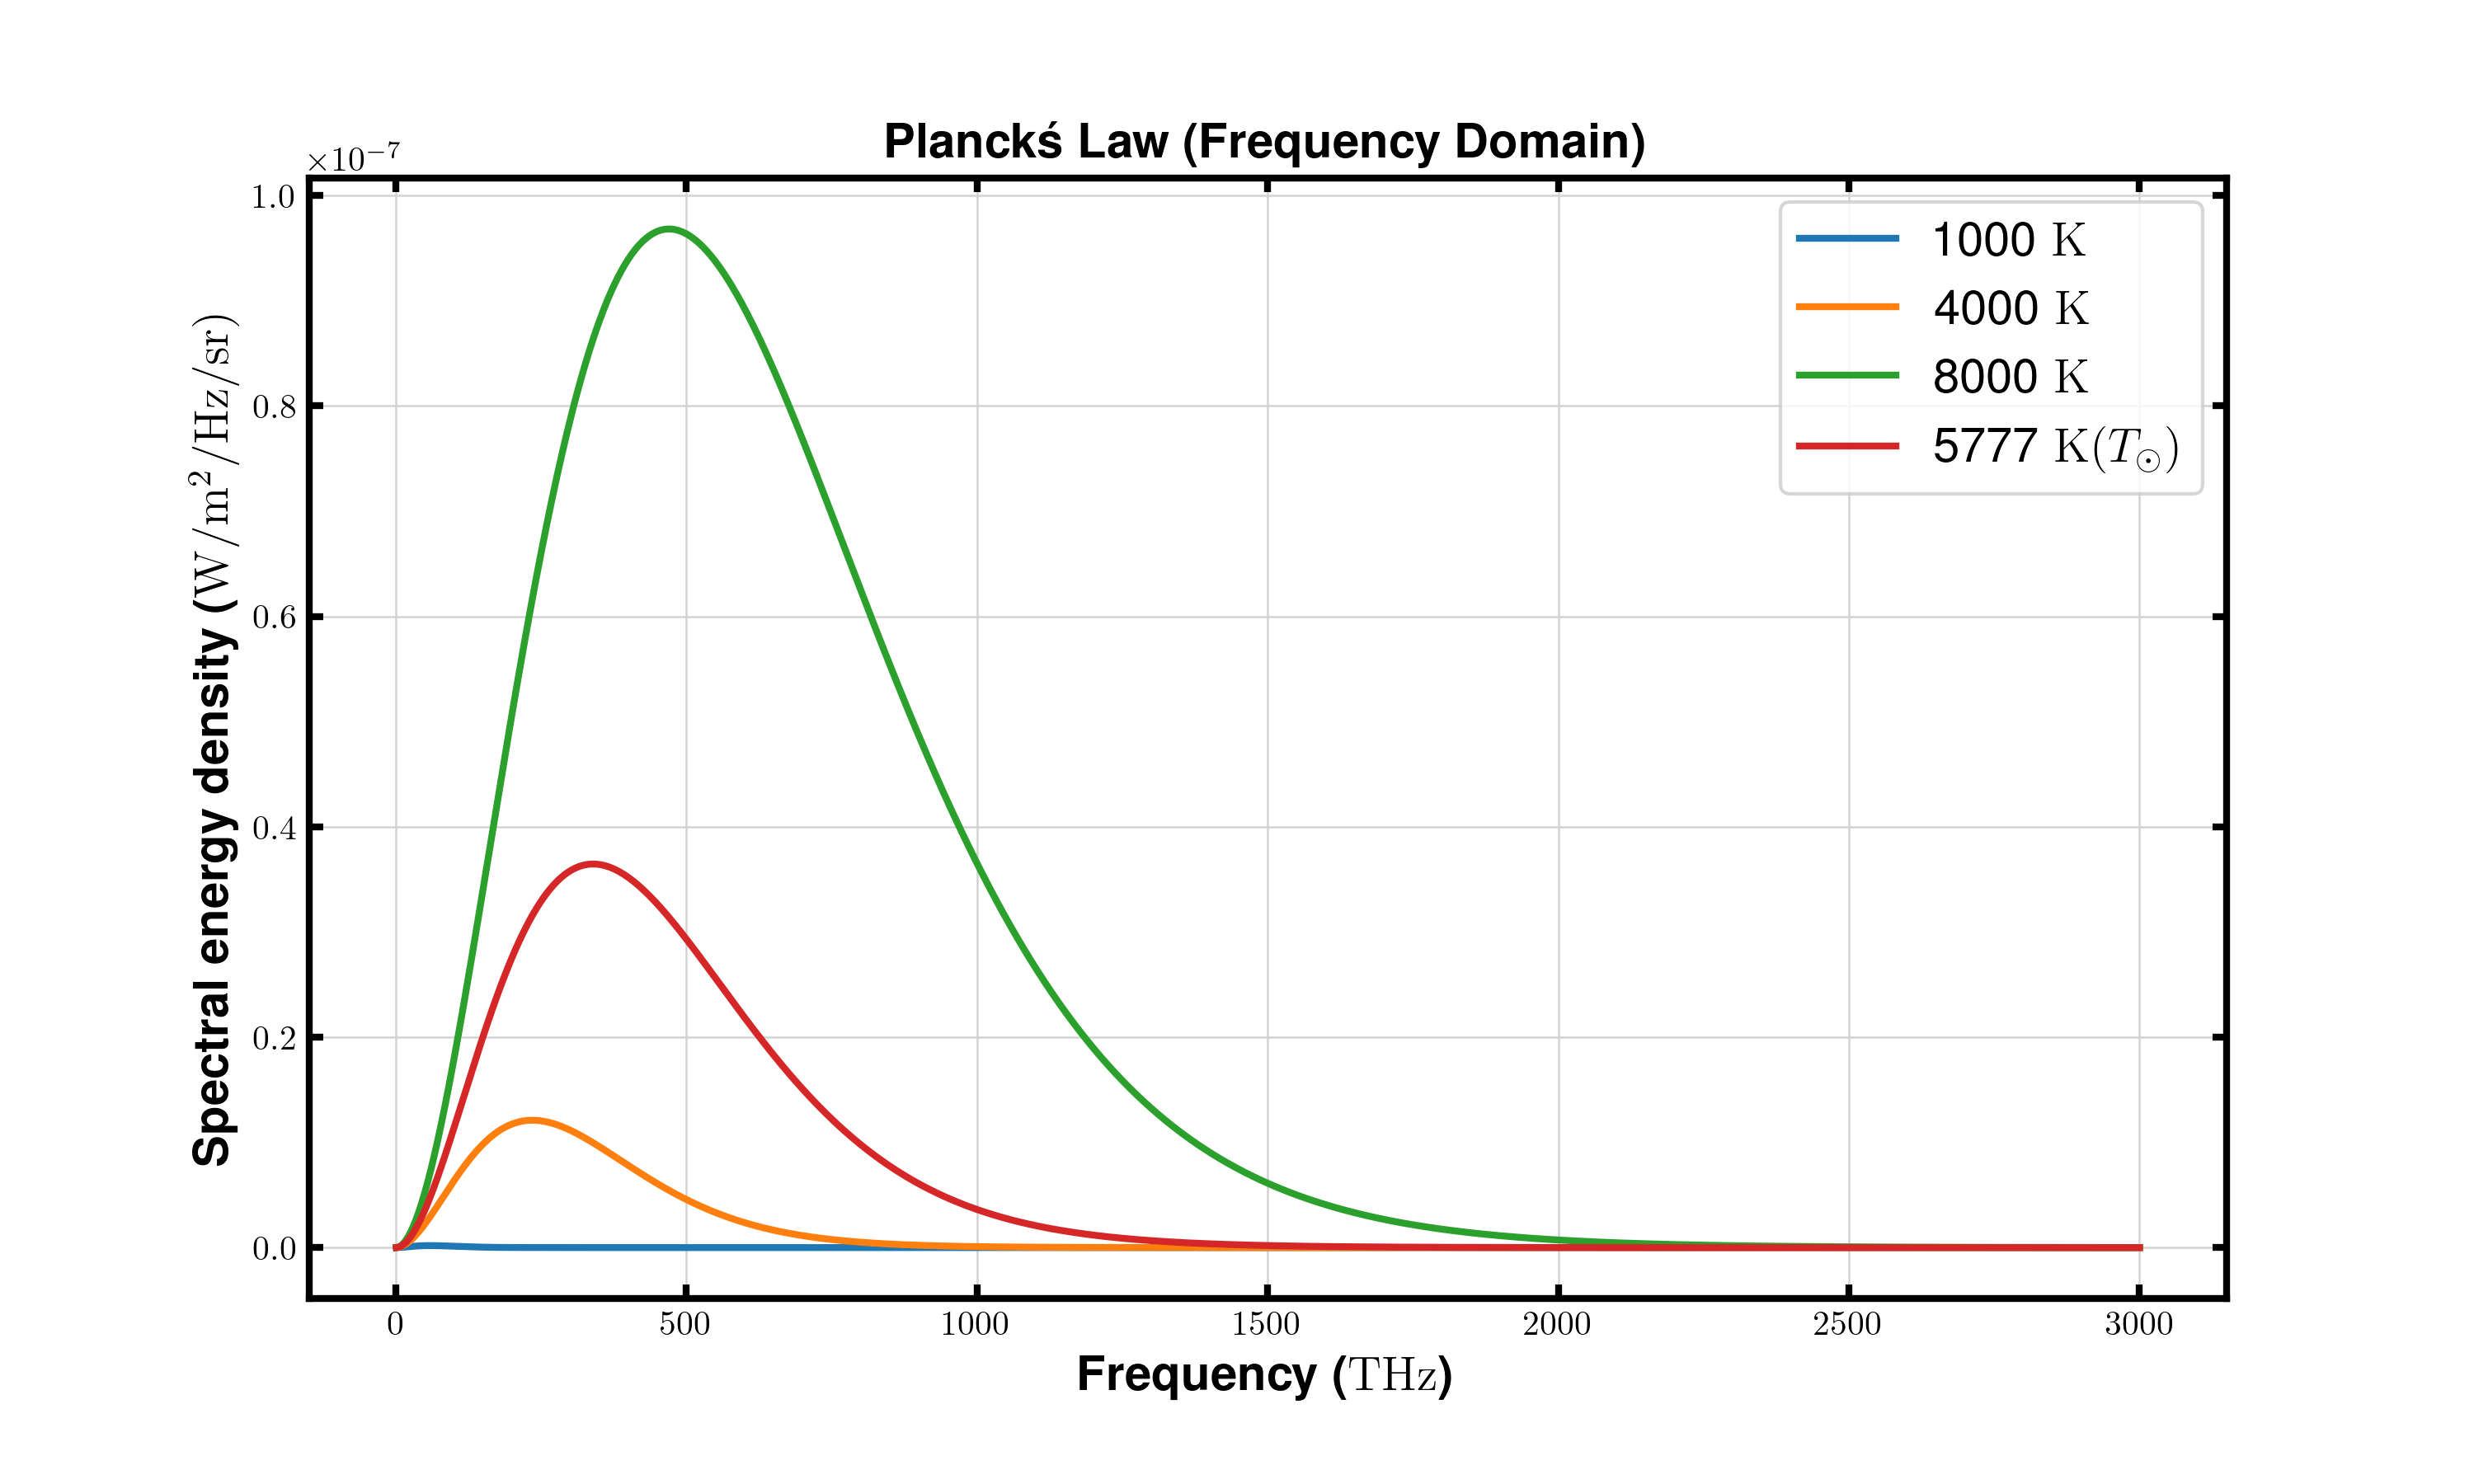
\includegraphics[scale=.5]{fig/Plank_law.png}
 \caption{Spectral energy density vs frequency for 3 different temperature and for the sun}
 \label{fig2.2}
 \end{figure}

 In figure \ref{fig2.2} the spectral energy density of four different temperatures as a function of frequency have been shown.

 \subsection{Exercise 2.8}

 The Sun undergoes an 11-year cycle during which its magnetic field reverses, resulting in distinct phases of solar activity. These phases include periods of minimum solar activity, known as the Quiet Sun, and times of maximum solar activity, referred to as the Active Sun. These cycles have a significant impact on radio emissions, with heightened radio emissions observed during the Active Sun phase and reduced emissions during the Quiet Sun phase. The variation in radio emissions between these two phases is illustrated in figure \ref{fig2.3}.

 \begin{figure}[H]
 \centering
 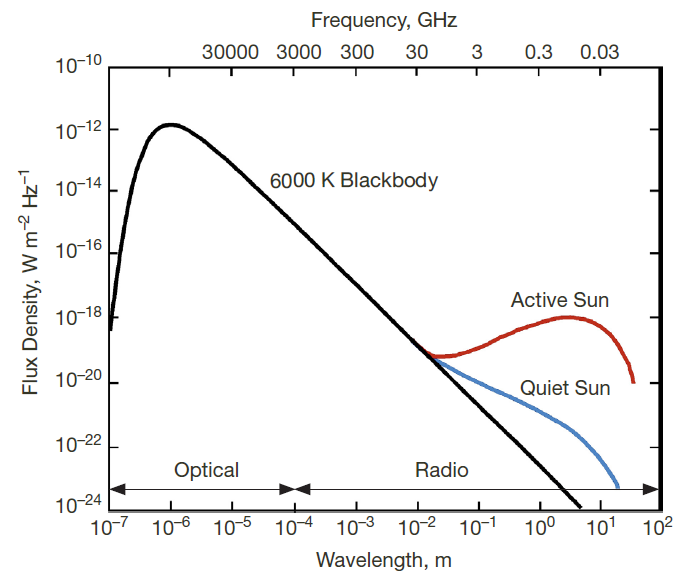
\includegraphics[scale=.5]{fig/sunRadioSpectrum.png}
 \caption{Flux density of radiations emitted by the Sun during its active and quiet phases.\parencite[Image credit][]{activequitesun}}
 \label{fig2.3}
 \end{figure}


 \subsection{Exercise 2.9}

 The observed size of the Sun is contingent upon the frequency of observation. At extremely low frequencies (below 0.1 GHz), the Sun's apparent size increases significantly. Consequently, this phenomenon causes the Sun to appear larger when examining the corona in comparison to studying the photosphere\parencite{sizeofsun}. 

 \subsection{Data processing}

 \subsubsection{Declination scan}
 \label{S2.2}

A declination scan involves keeping a constant Right Ascension setting on the telescope while adjusting the telescope's Declination by computer. This adjustment ensures that as the sun moves across the fixed Right Ascension of our telescope, we obtain a comprehensive scan of the entire Sun. To align the telescope with the Sun, we utilize the shadow cast by the detector on the dish. This process is highly dependent on favorable weather conditions because the telescope requires manual positioning. The resulting raster scan of the Sun is achieved through vertical scanning in Declination. The data gathered during this observation sequence serves as the foundation for generating a radio image of the Sun. Additionally, the telescope's scanning can be visualized by plotting its Declination against Right Ascension, as shown in the figure 

 \begin{figure}[H]
 \centering
 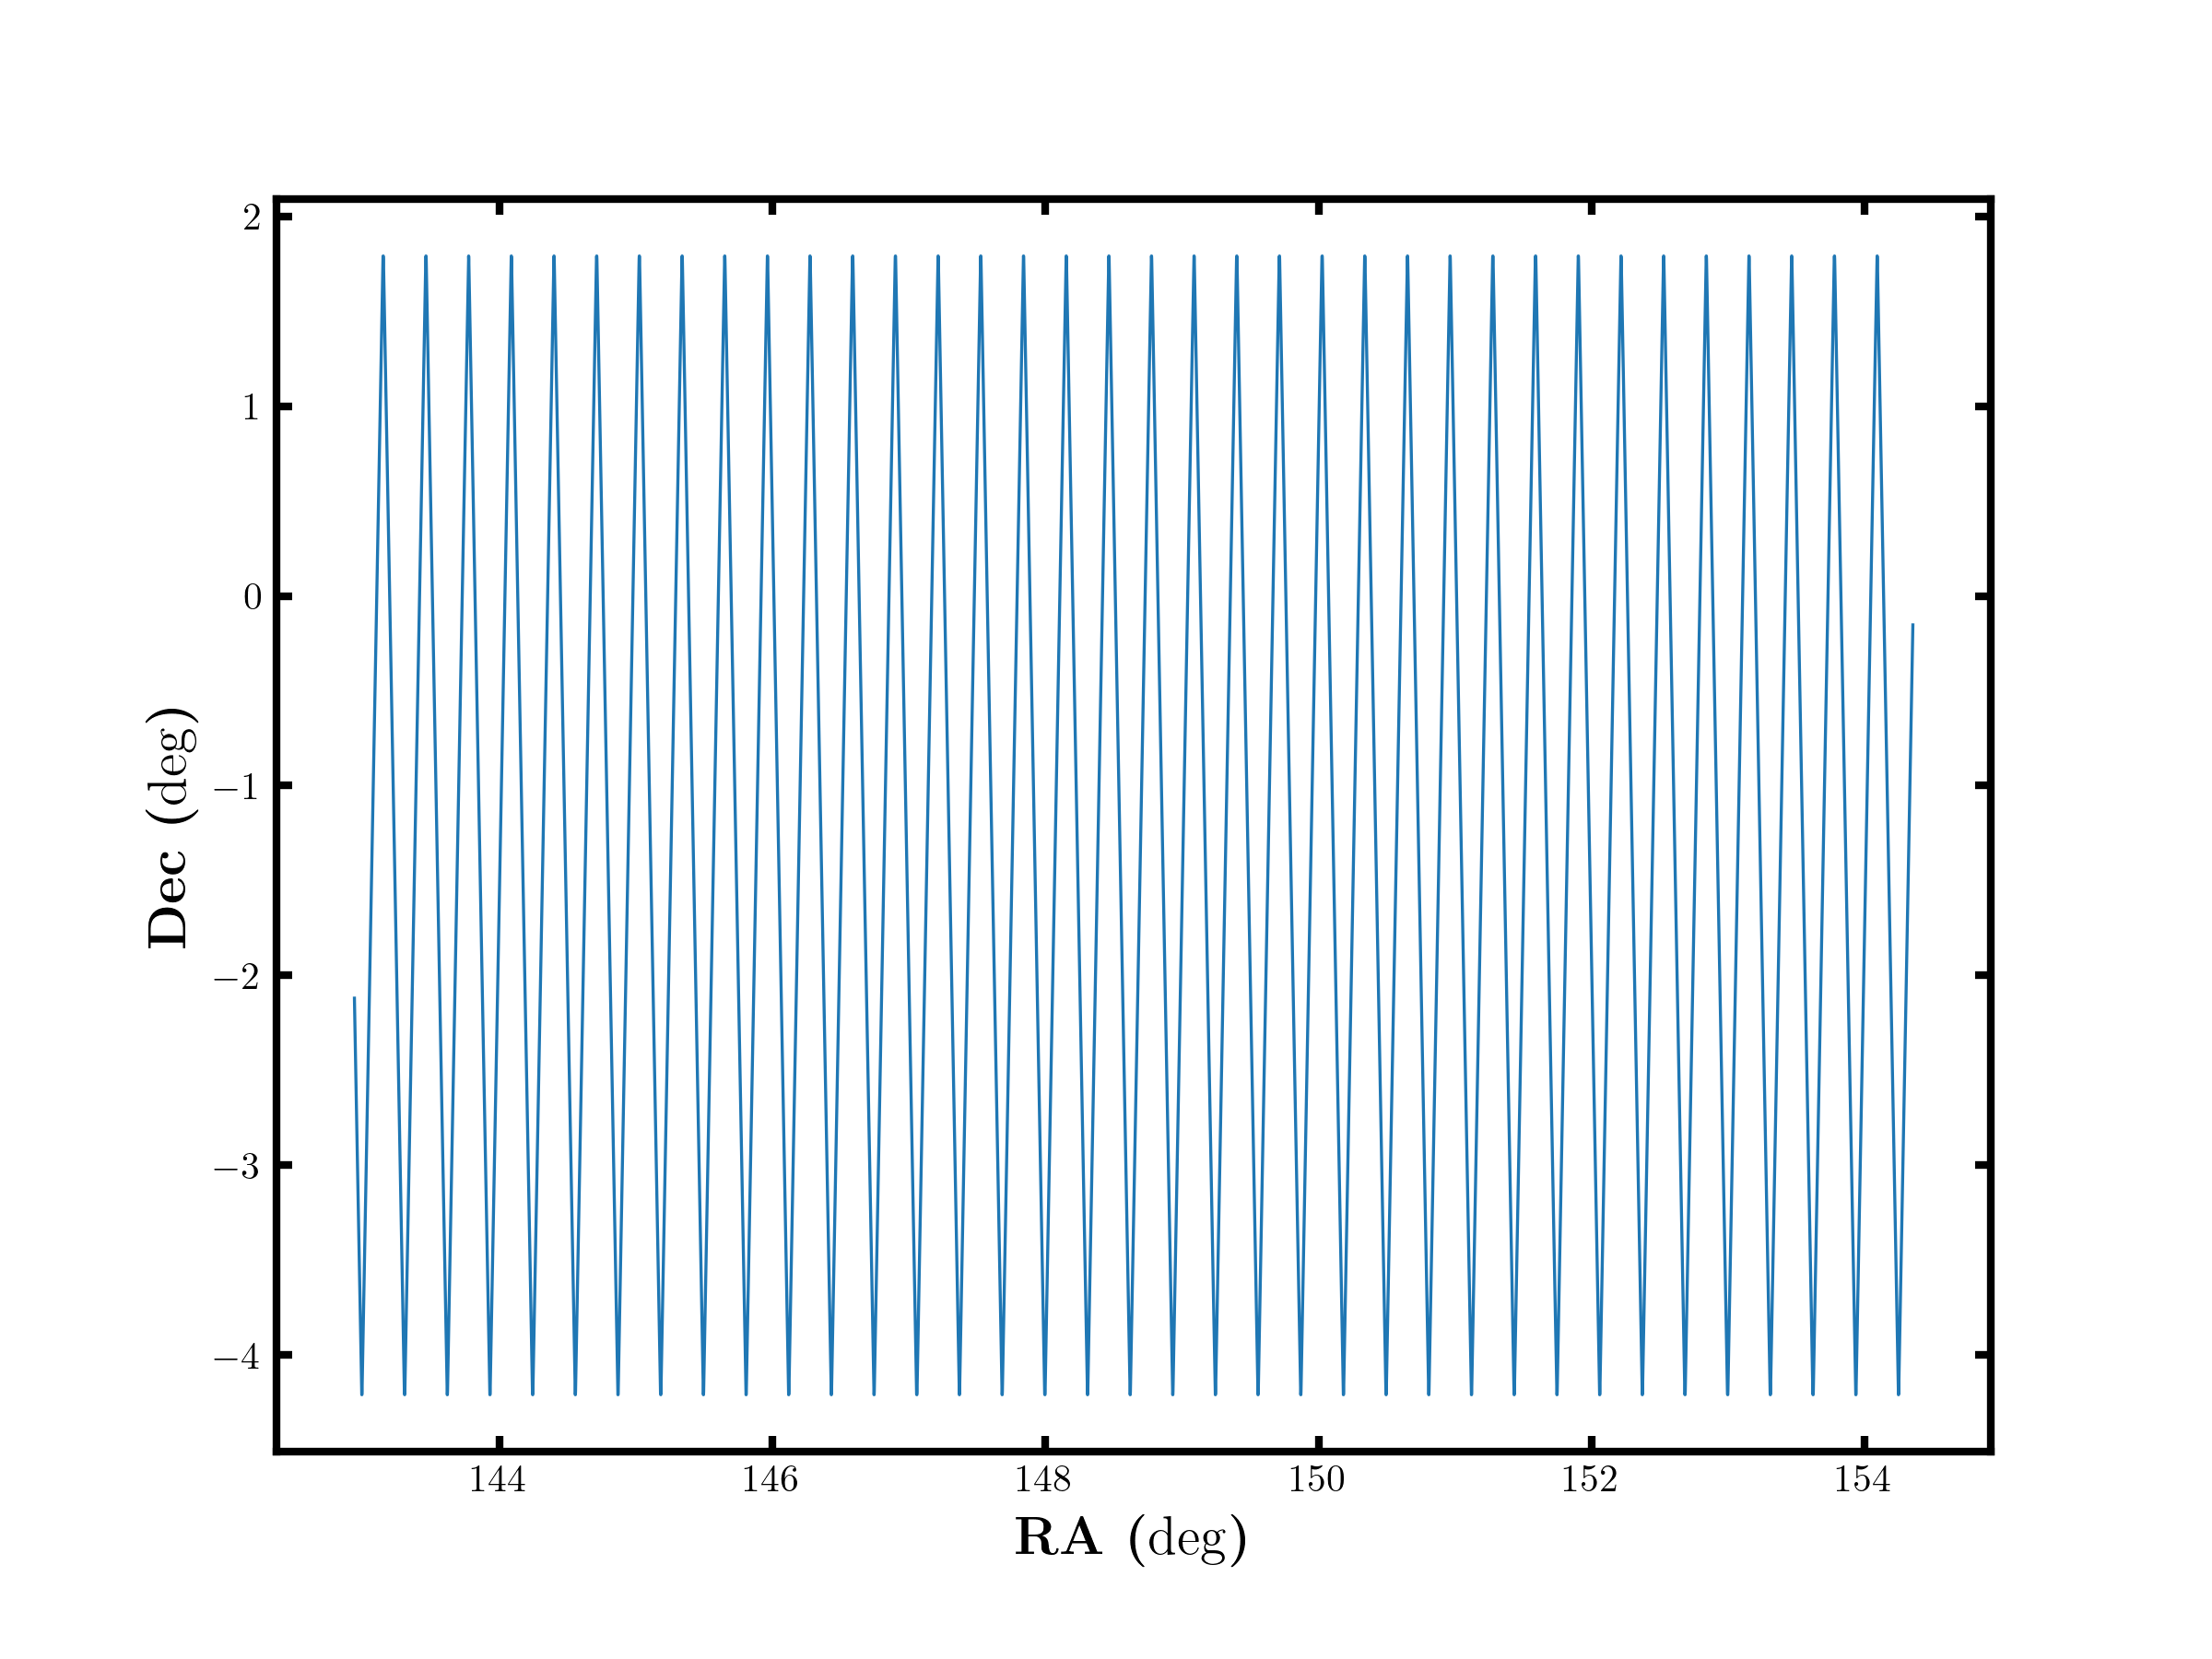
\includegraphics[scale=.6]{fig/decscan.png}
 \caption{The plot illustrates how telescopes move during the declination scan by tracking changes in Right Ascension (RA) on the x-axis and Declination (Dec) on the y-axis.}
 \label{fig2.4}
 \end{figure}

 It displays the anticipated zigzag pattern. When the Sun enters the telescope's beam, it registers an intensity signal. Alongside this, a significant amount of noise is recorded, which is shown in a plot of signal amplitude over time in the raw data figure \ref{fig2.5}.

 \begin{figure}[H]
 \centering
 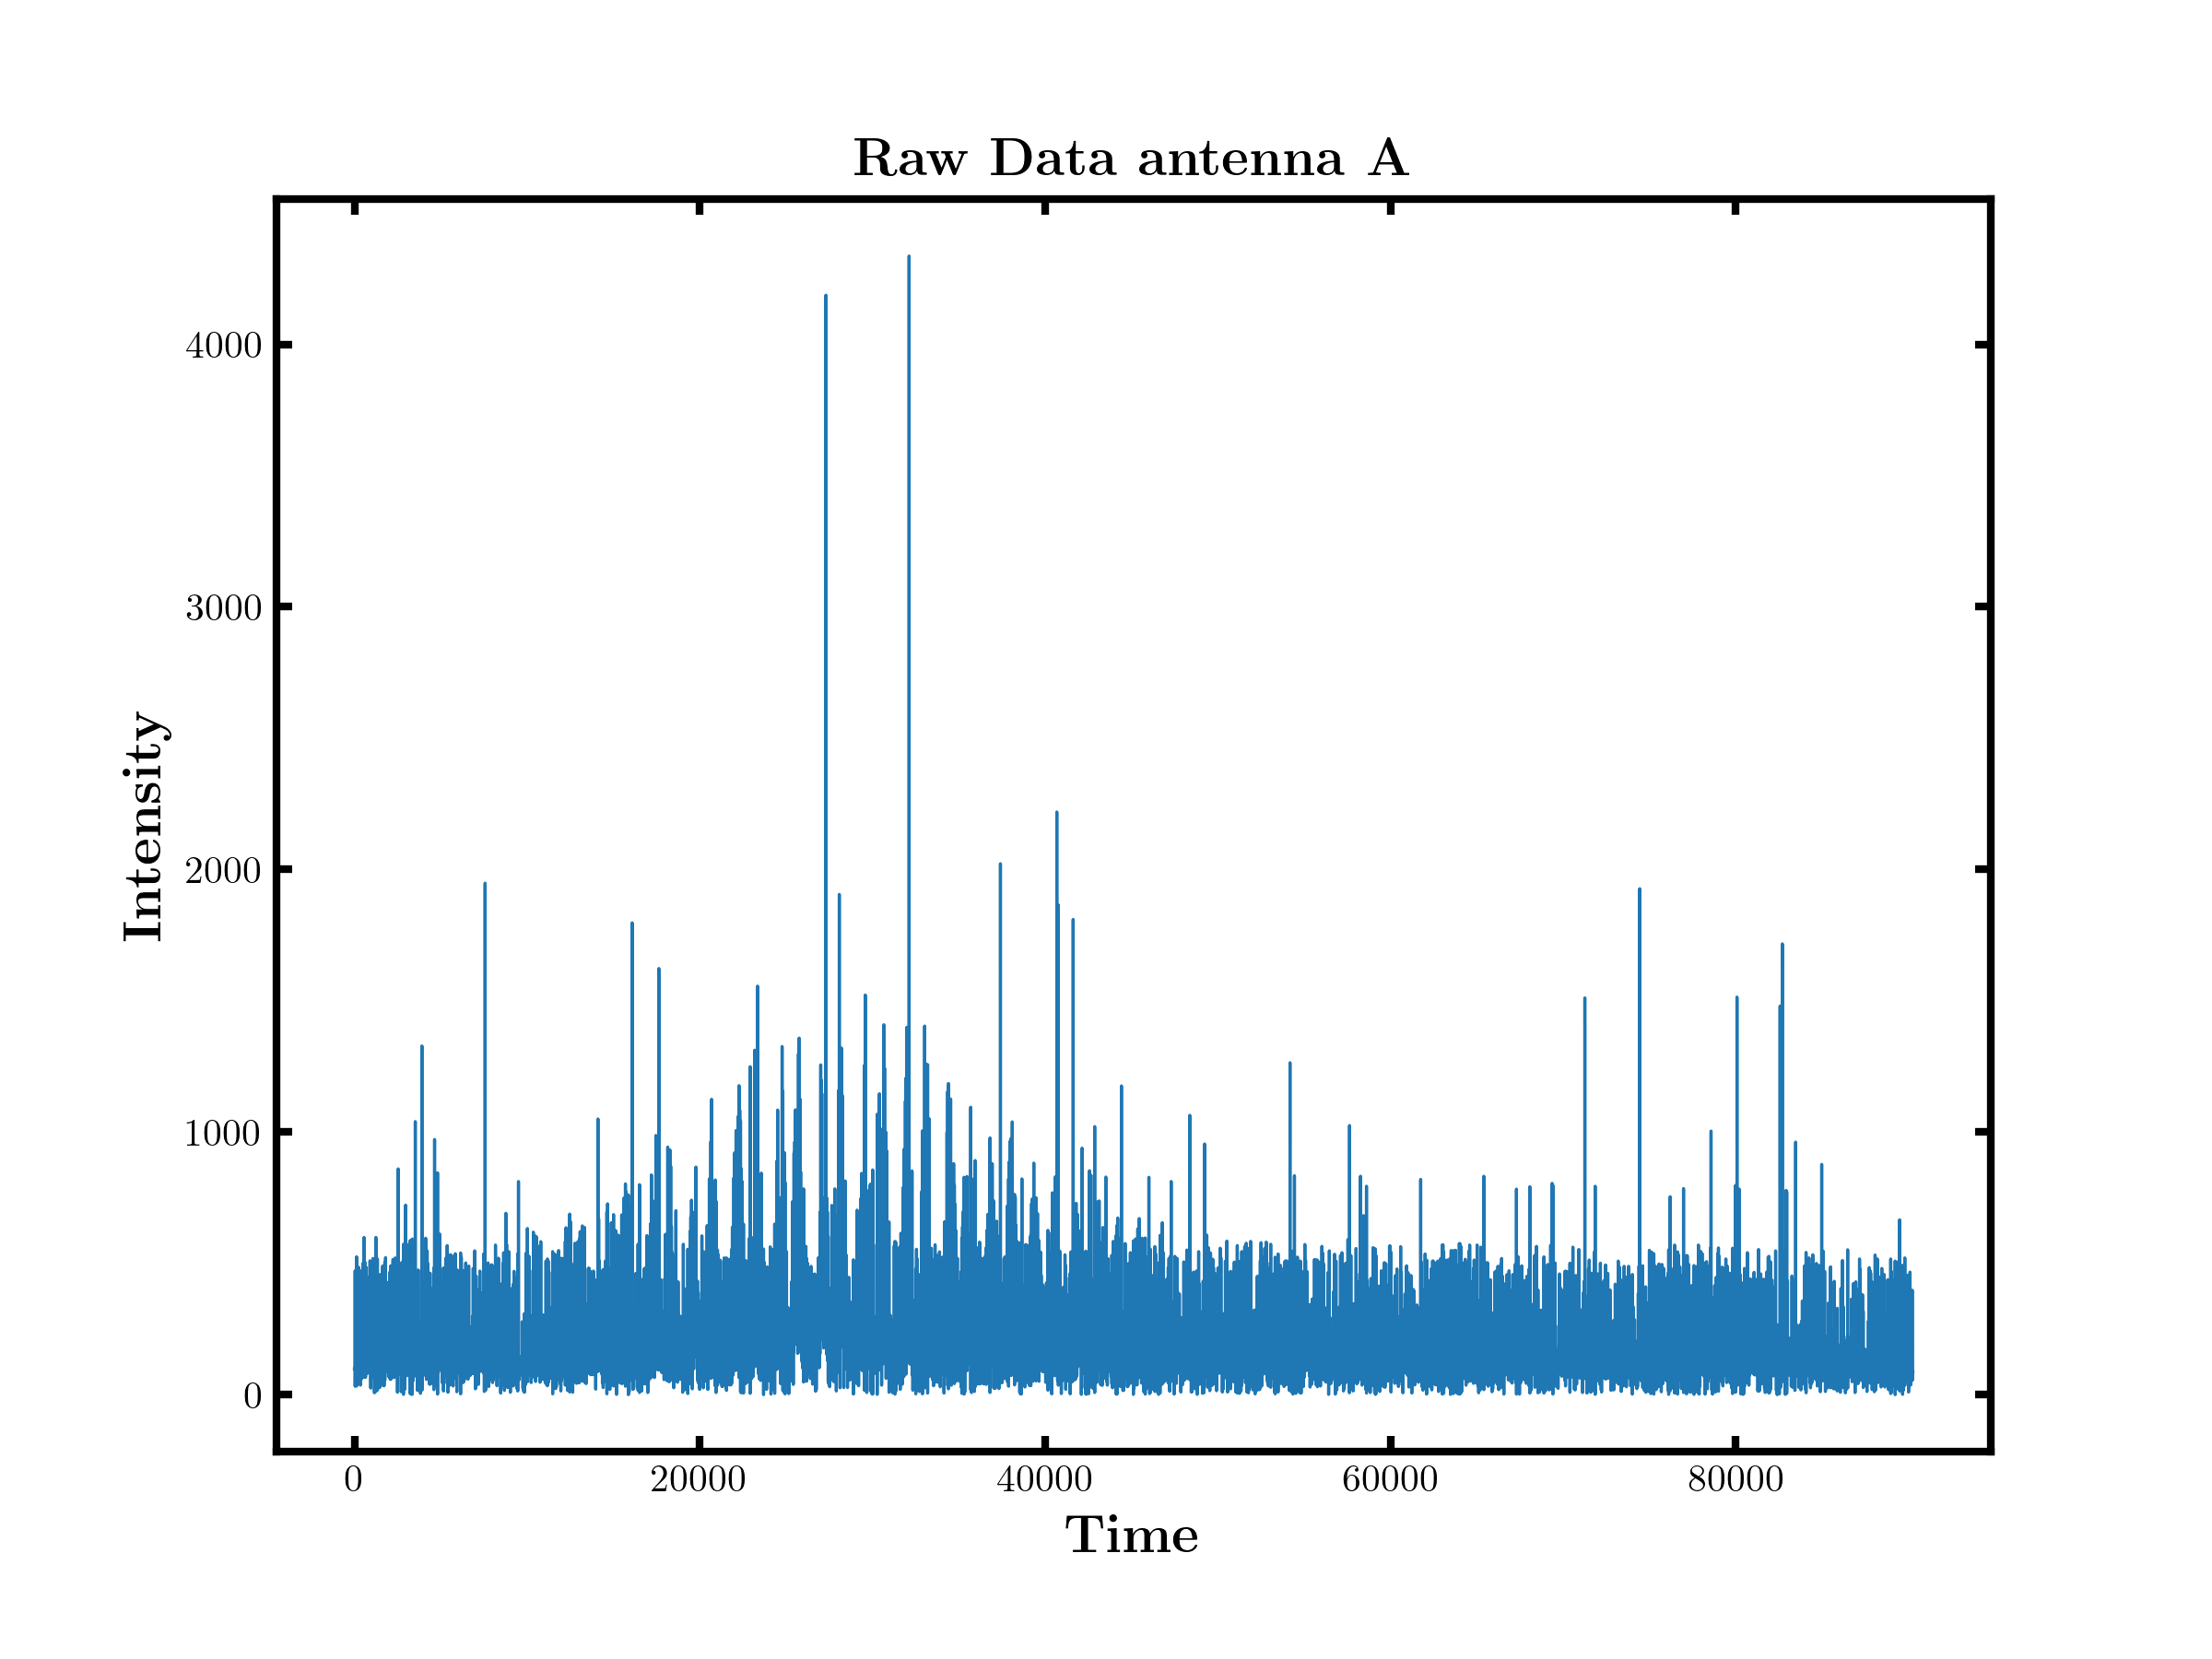
\includegraphics[scale=.6]{fig/Raw_Data_antena_A.png}
 \caption{Intensity vs time plot of the raw data of the declination scan(Antenna A).}
 \label{fig2.5}
 \end{figure}

 To eliminate this noise, a data cleaning process is employed\parencite{lecturenote}. Initially, the flux data array is compared to itself, but with each entry shifted one position to the right. Any elements with an absolute difference greater than 60 are subsequently removed. The same procedure is applied to the both real and imaginary components of the visibility function, with a maximum allowable absolute difference of 30. This noise reduction process is repeated eight times, resulting in cleaned data, as shown in figure \ref{fig2.6} for antenna A and figure \ref{fig2.7} for antenna B.

 \begin{figure}[H]
    \centering
    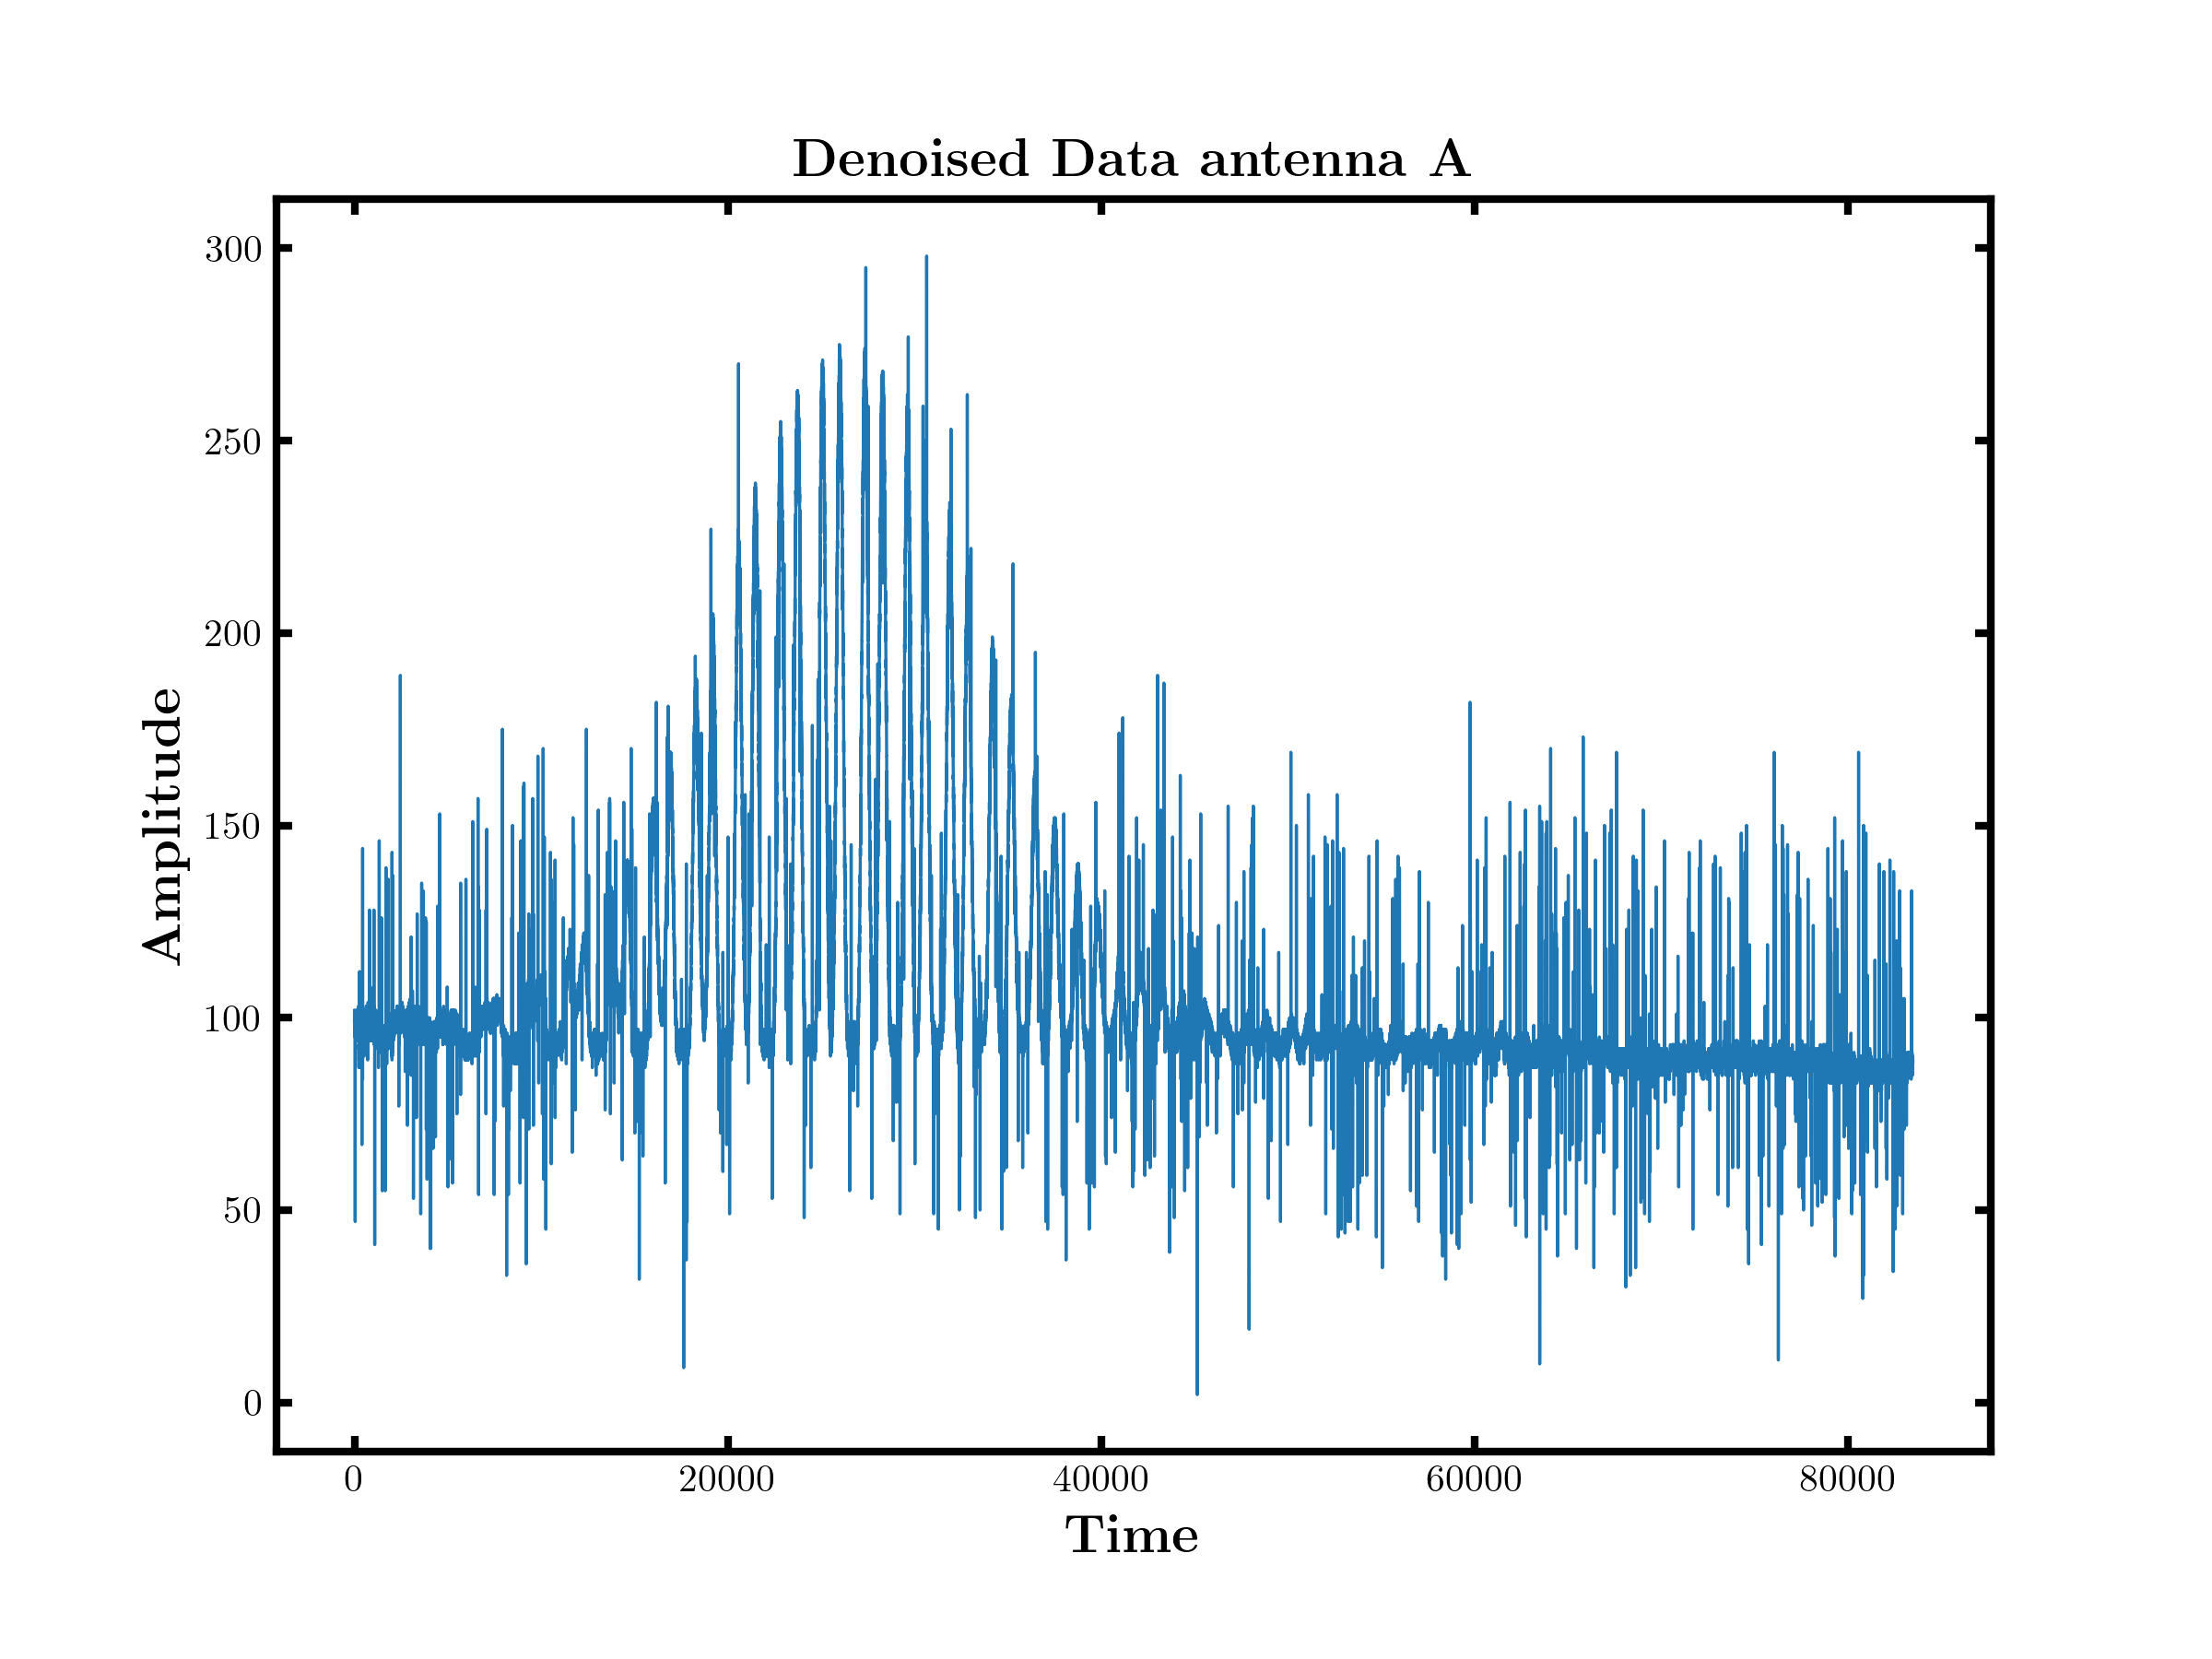
\includegraphics[scale=.6]{fig/Denoised_Data_antena_A.png}
    \caption{Intensity vs time plot of the denoised data of the declination scan of antenna A.}
    \label{fig2.6}
 \end{figure}

 \begin{figure}[H]
    \centering
    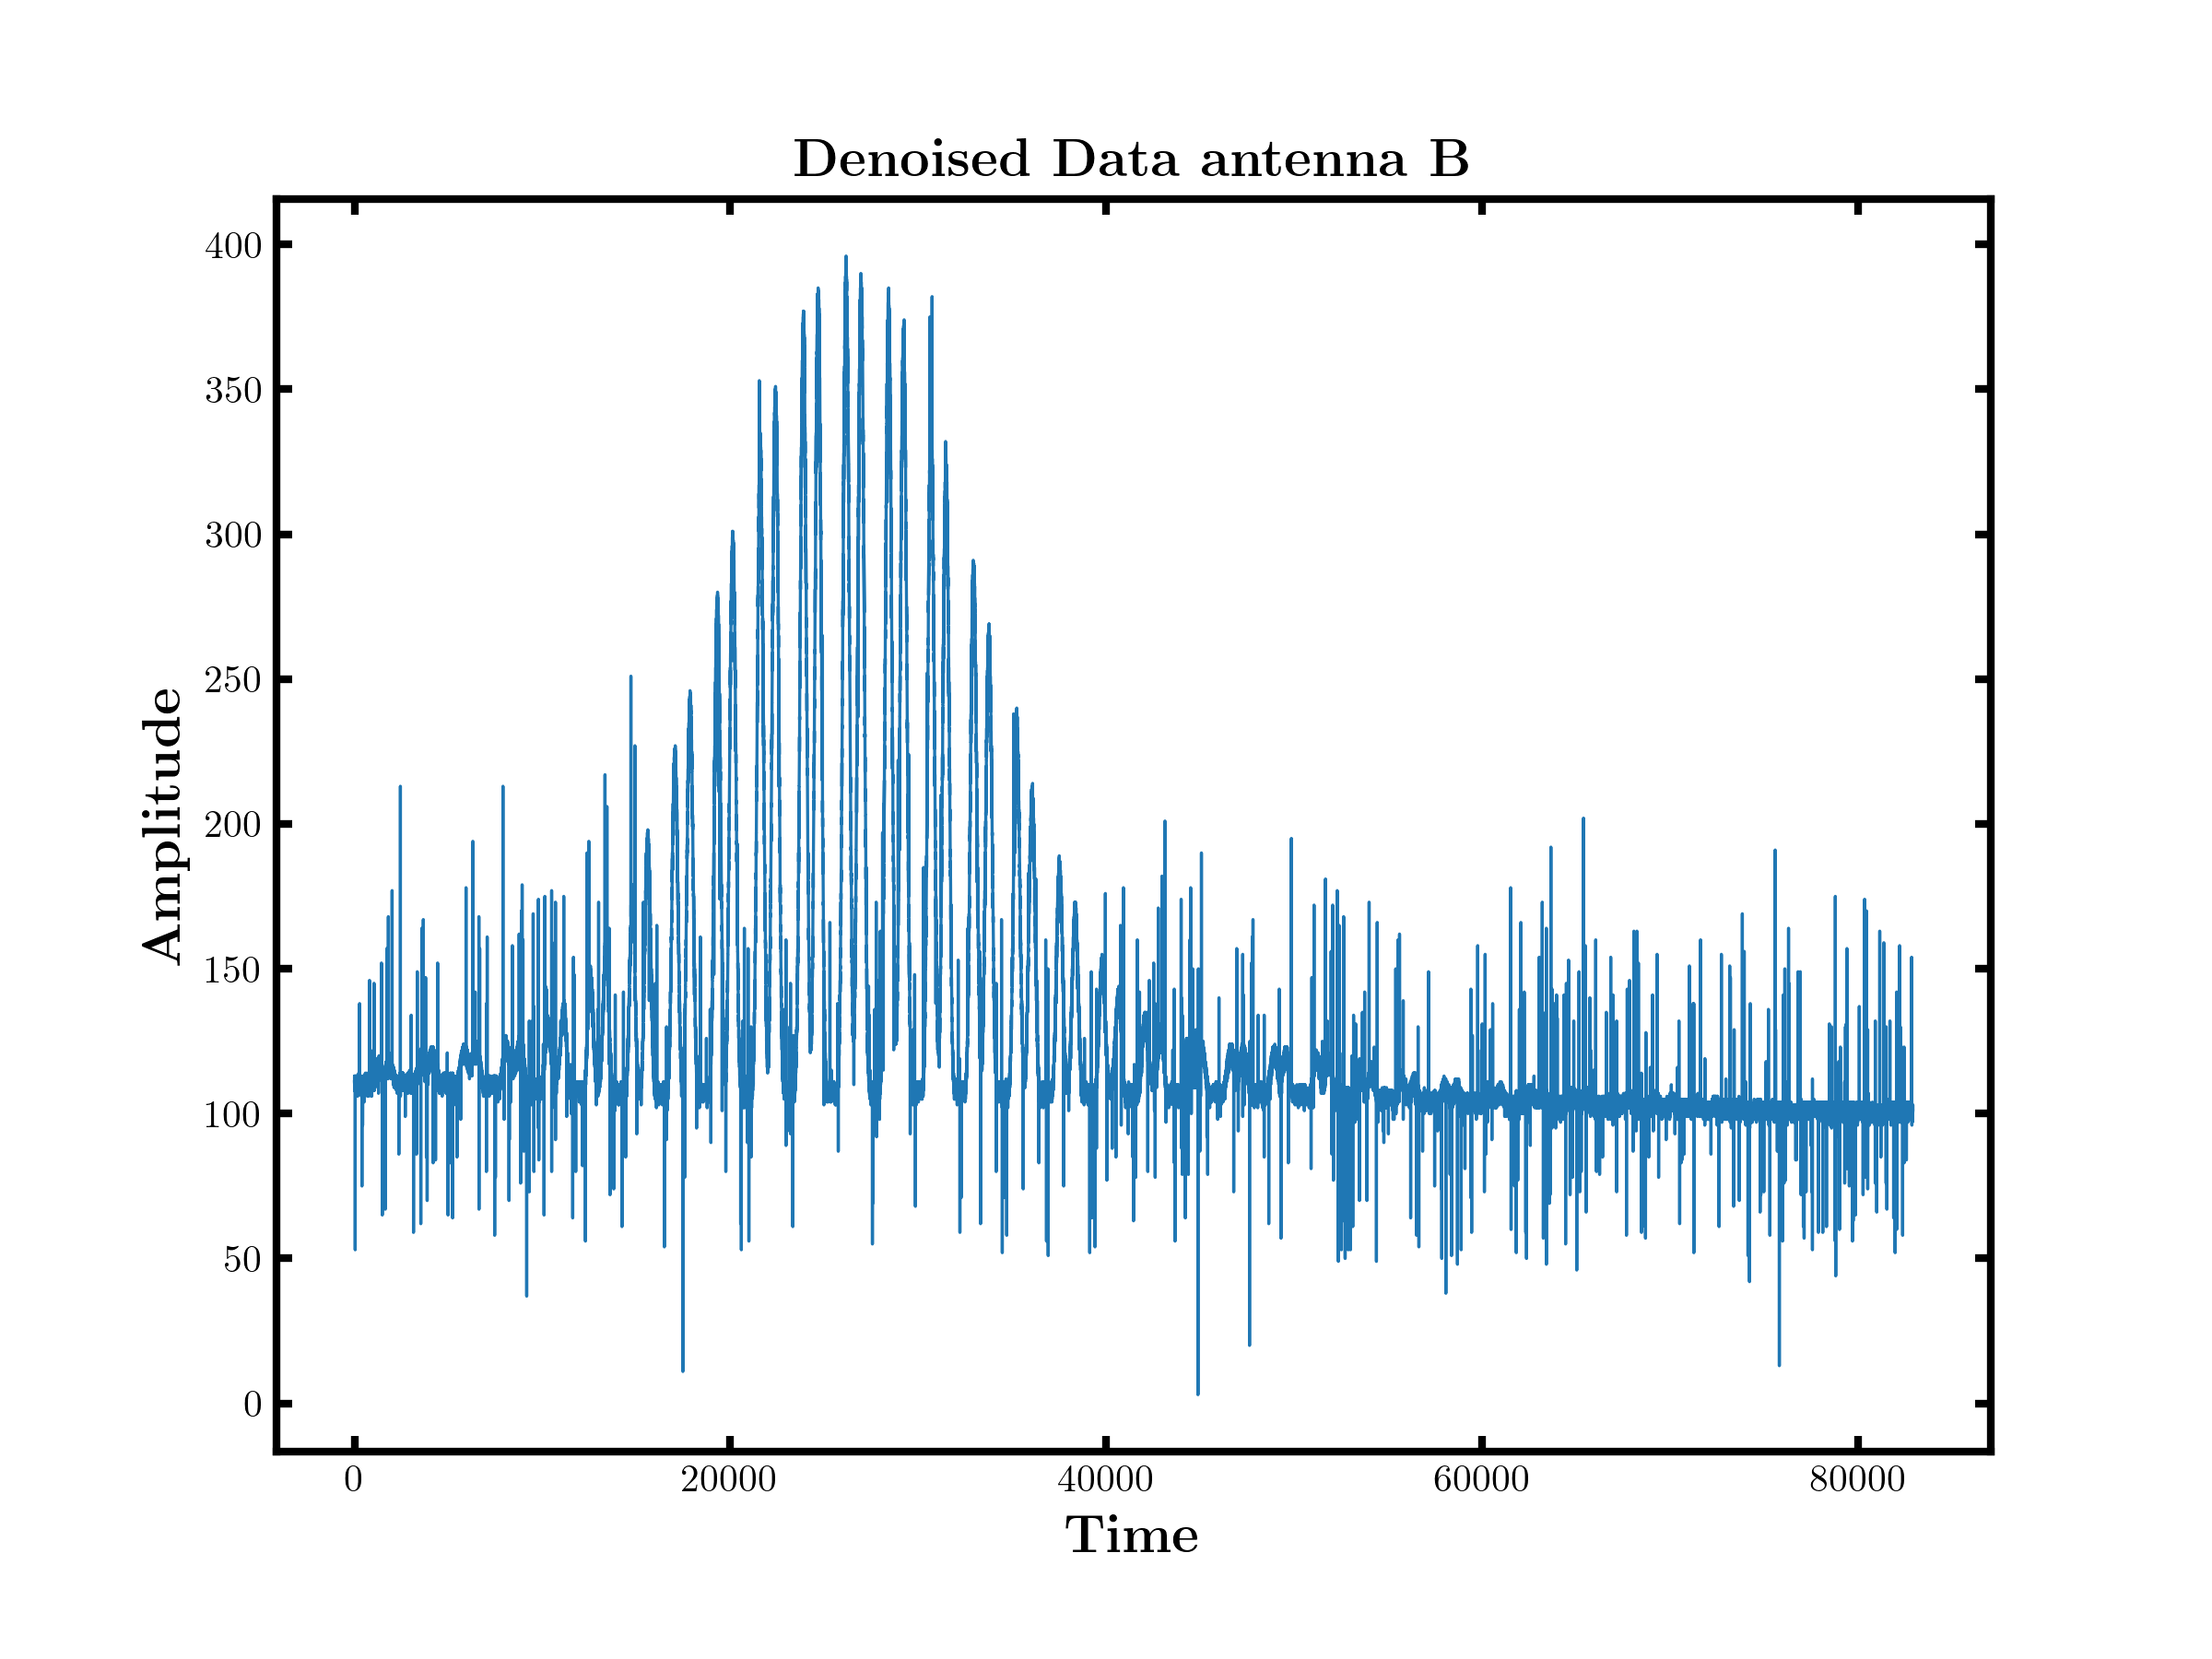
\includegraphics[scale=.6]{fig/Denoised_Data_antena_B.png}
    \caption{Intensity vs time plot of the denoised data of the declination scan of antenna B.}
    \label{fig2.7}
 \end{figure}

 In the processed spectra without noise, variations in intensity can be observed as the Sun traverses the telescope's beam. After examining the plot, the data range has been adjusted to cover the time interval from 5000 to 50000 seconds.

 By using the denoised data and the code provided in \parencite{lecturenote} a 2D image of the sun has been created for both antenna. these images is shown in figure \ref{fig2.89} 
 \begin{figure}[H]
     \centering
     \begin{subfigure}{.45\textwidth}
         \centering
         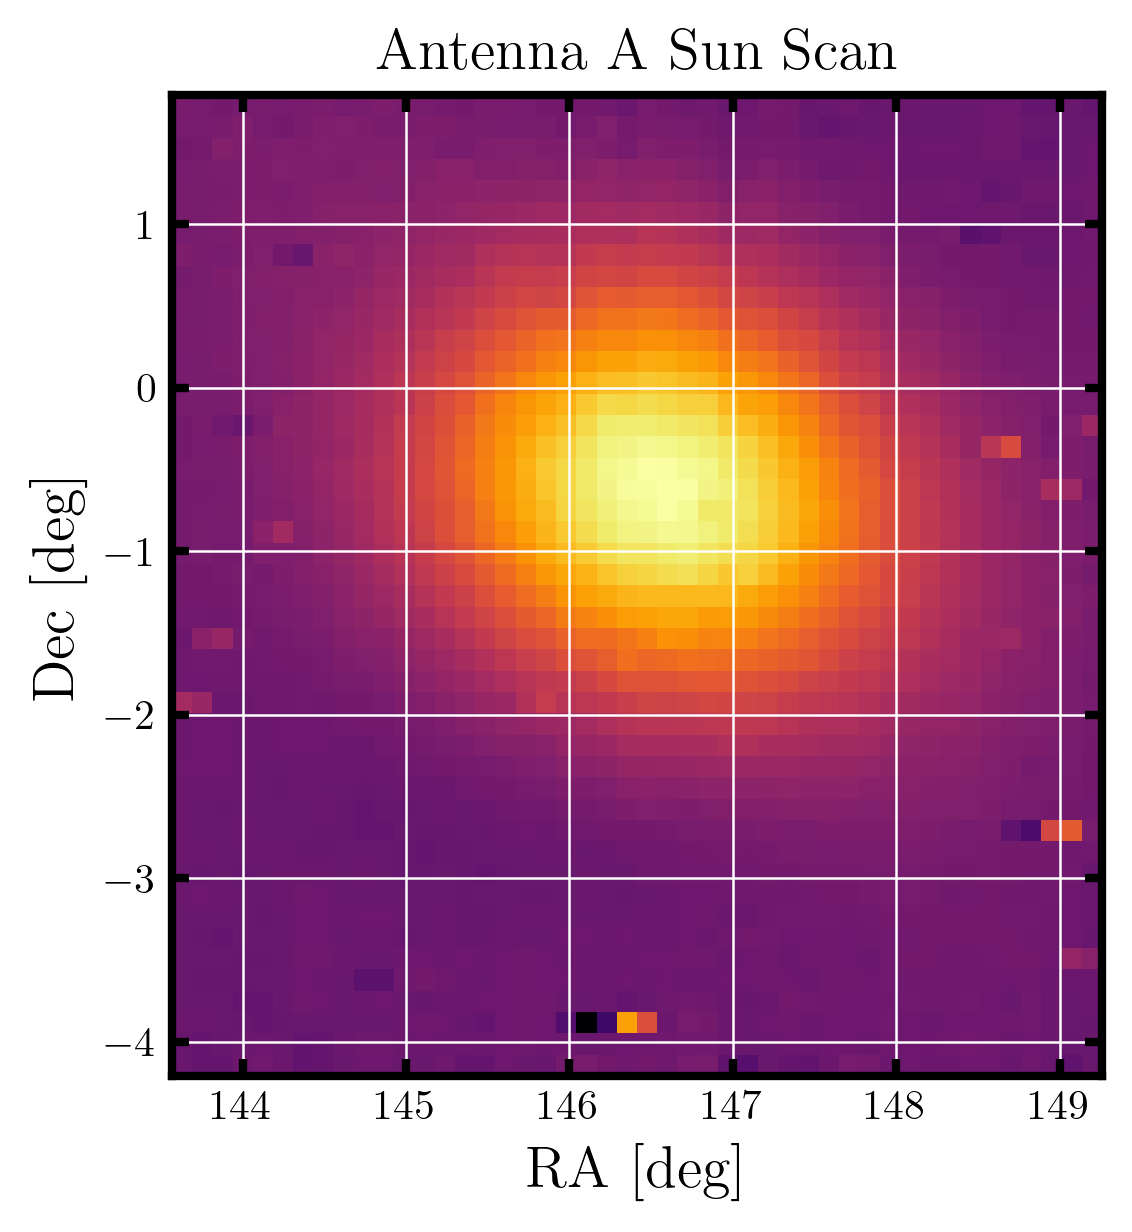
\includegraphics[width=\textwidth]{fig/7.AntennaAscan.png}
         \caption{Sun scan antenna A}
         \label{fig2.8}
     \end{subfigure}
     \hfill
     \begin{subfigure}{.45\textwidth}
         \centering
         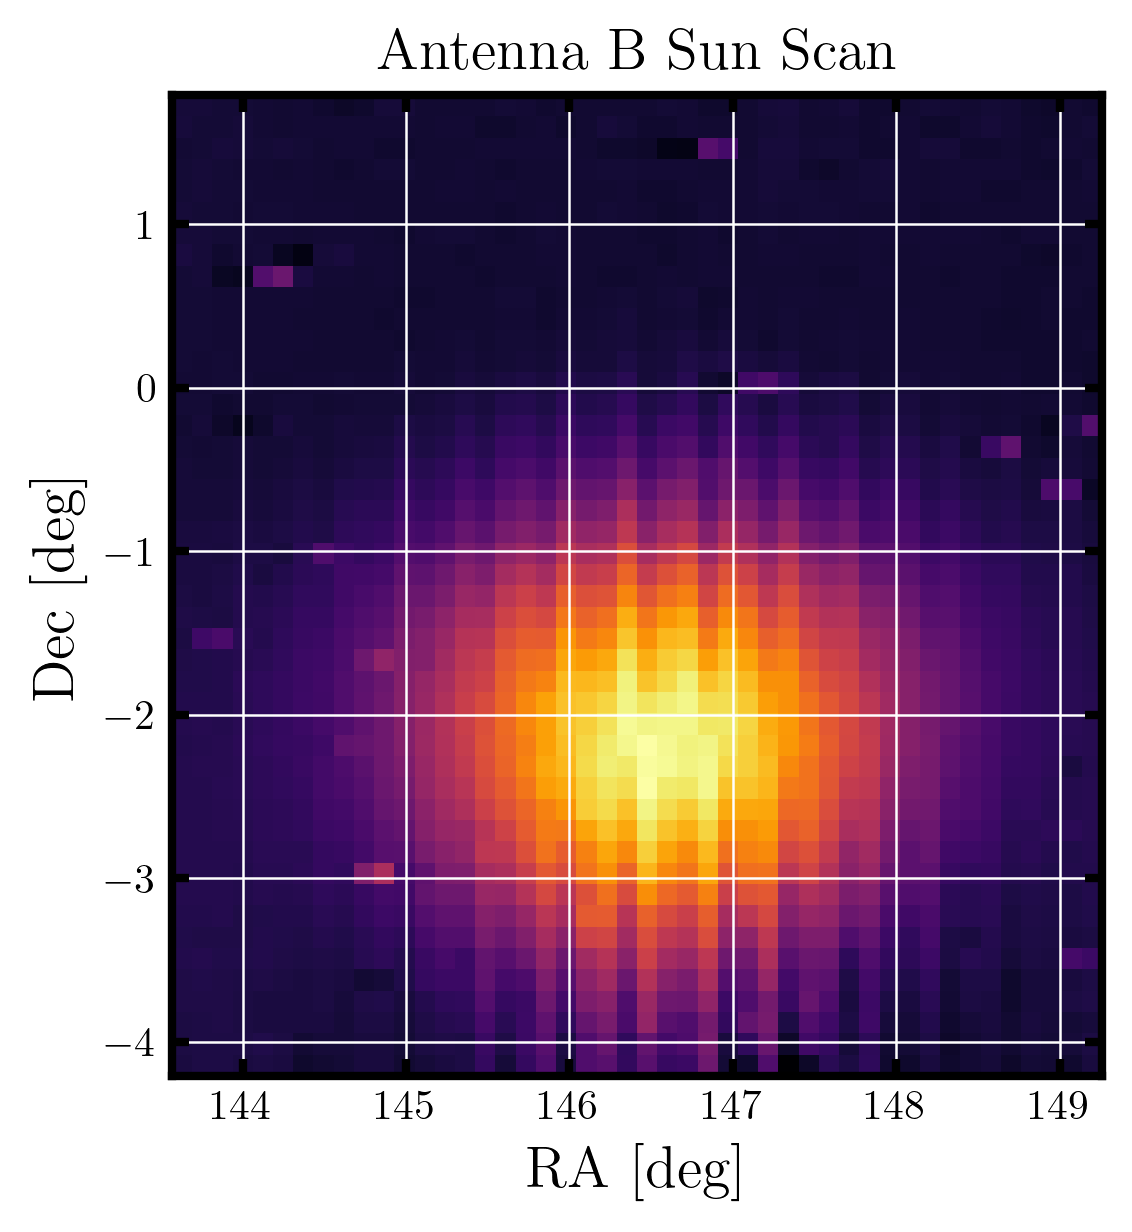
\includegraphics[width=\textwidth]{fig/8.AntennaBscan.png}
         \caption{Sun scan antenna B}
         \label{fig2.9}
     \end{subfigure}
        \caption{2D image of the sun obtained by two antennas}
        \label{fig2.89}
 \end{figure}

 The image of antenna B is noisy however, the one from antenna A is almost clear. from figure \ref{fig2.89}, it is clear that the angular resolution of a single dish is poor. This can be further confirmed by cross-correlation of data received from both antennas. The width of the interference pattern will provide us with information about the angular resolution of our telescope setup (interferometer twin telescope). It is important to note that if we were to increase the distance between the antennas (referred to as the baseline), the interference fringes would become narrower, leading to a better angular resolution.   
 \begin{figure}[H]
    \centering
    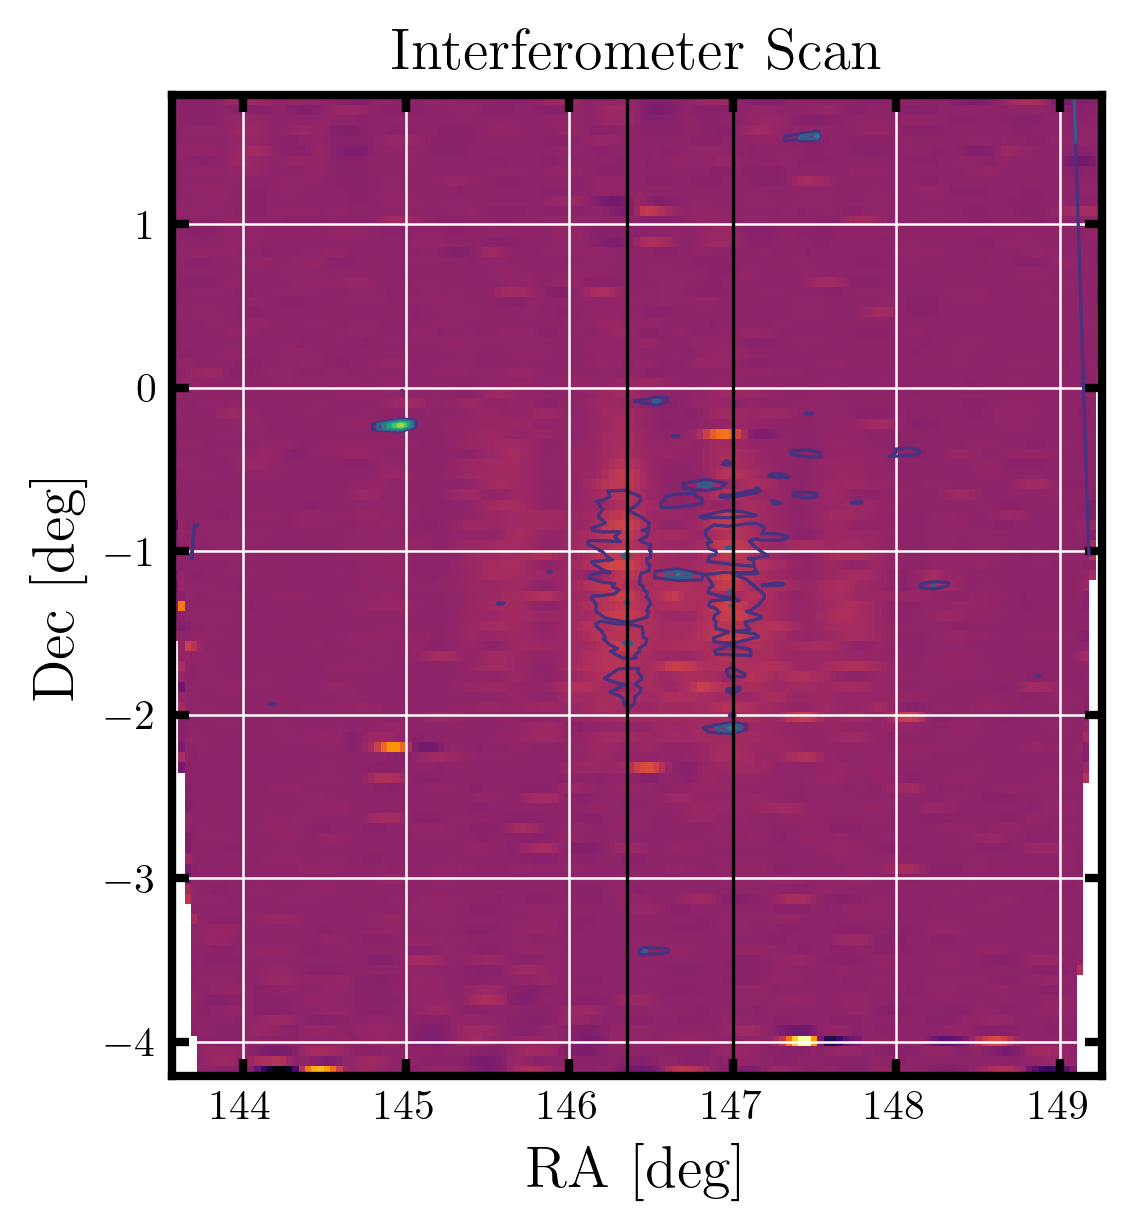
\includegraphics[scale=1]{fig/9.Interfscan.png}
    \caption{Interference pattern obtained by two antennas.}
    \label{fig2.10}
 \end{figure}

 The interference pattern can be seen in figure \ref{fig2.10}. From this, the values of two neighbouring maximum $\theta_1 = (146.4 \pm 0.1)$ and $\theta_2 = (147 \pm 0.1)$ can be obtained. This, results in an angular resolution of $\theta = (0.6 \pm 0.1)$. 

 From figure \ref{fig2.6} and \ref{fig2.7} the diameter of the sun can be estimated as roughly $2.1$ degree. By knowing the distance between the earth and the sun (1 AU) and this angel, Diameter of the sun can be calculated as following:

 \begin{equation}
 D = 1AU \times \theta = 150 \times 10^6 \times (2.1\pm 0.1) \times \dfrac{\pi}{180} = (5.5 \pm 0.3) \times 10^6 \mathrm{km} 
 \end{equation} 

 \subsubsection{Still scan}

 To perform a still scan of the sun, it is important to position the detector's shadow so that it aligns tangentially with the hole at the center of the dish. Simultaneously, the clamps on the mounts must remain fixed in place. During this stationary scan, the sun's movement is allowed to pass in front of the detectors without any movement of the antennas. This particular technique is employed to observe the fringe pattern created through interferometry. To reduce noise in the data, the same method described in section \ref{S2.2} for the declination scan is applied. The denoised data for antenna A and B can be seen in figure \ref{fig2.1112}.

 \begin{figure}[H]
     \centering
     \begin{subfigure}{.45\textwidth}
         \centering
         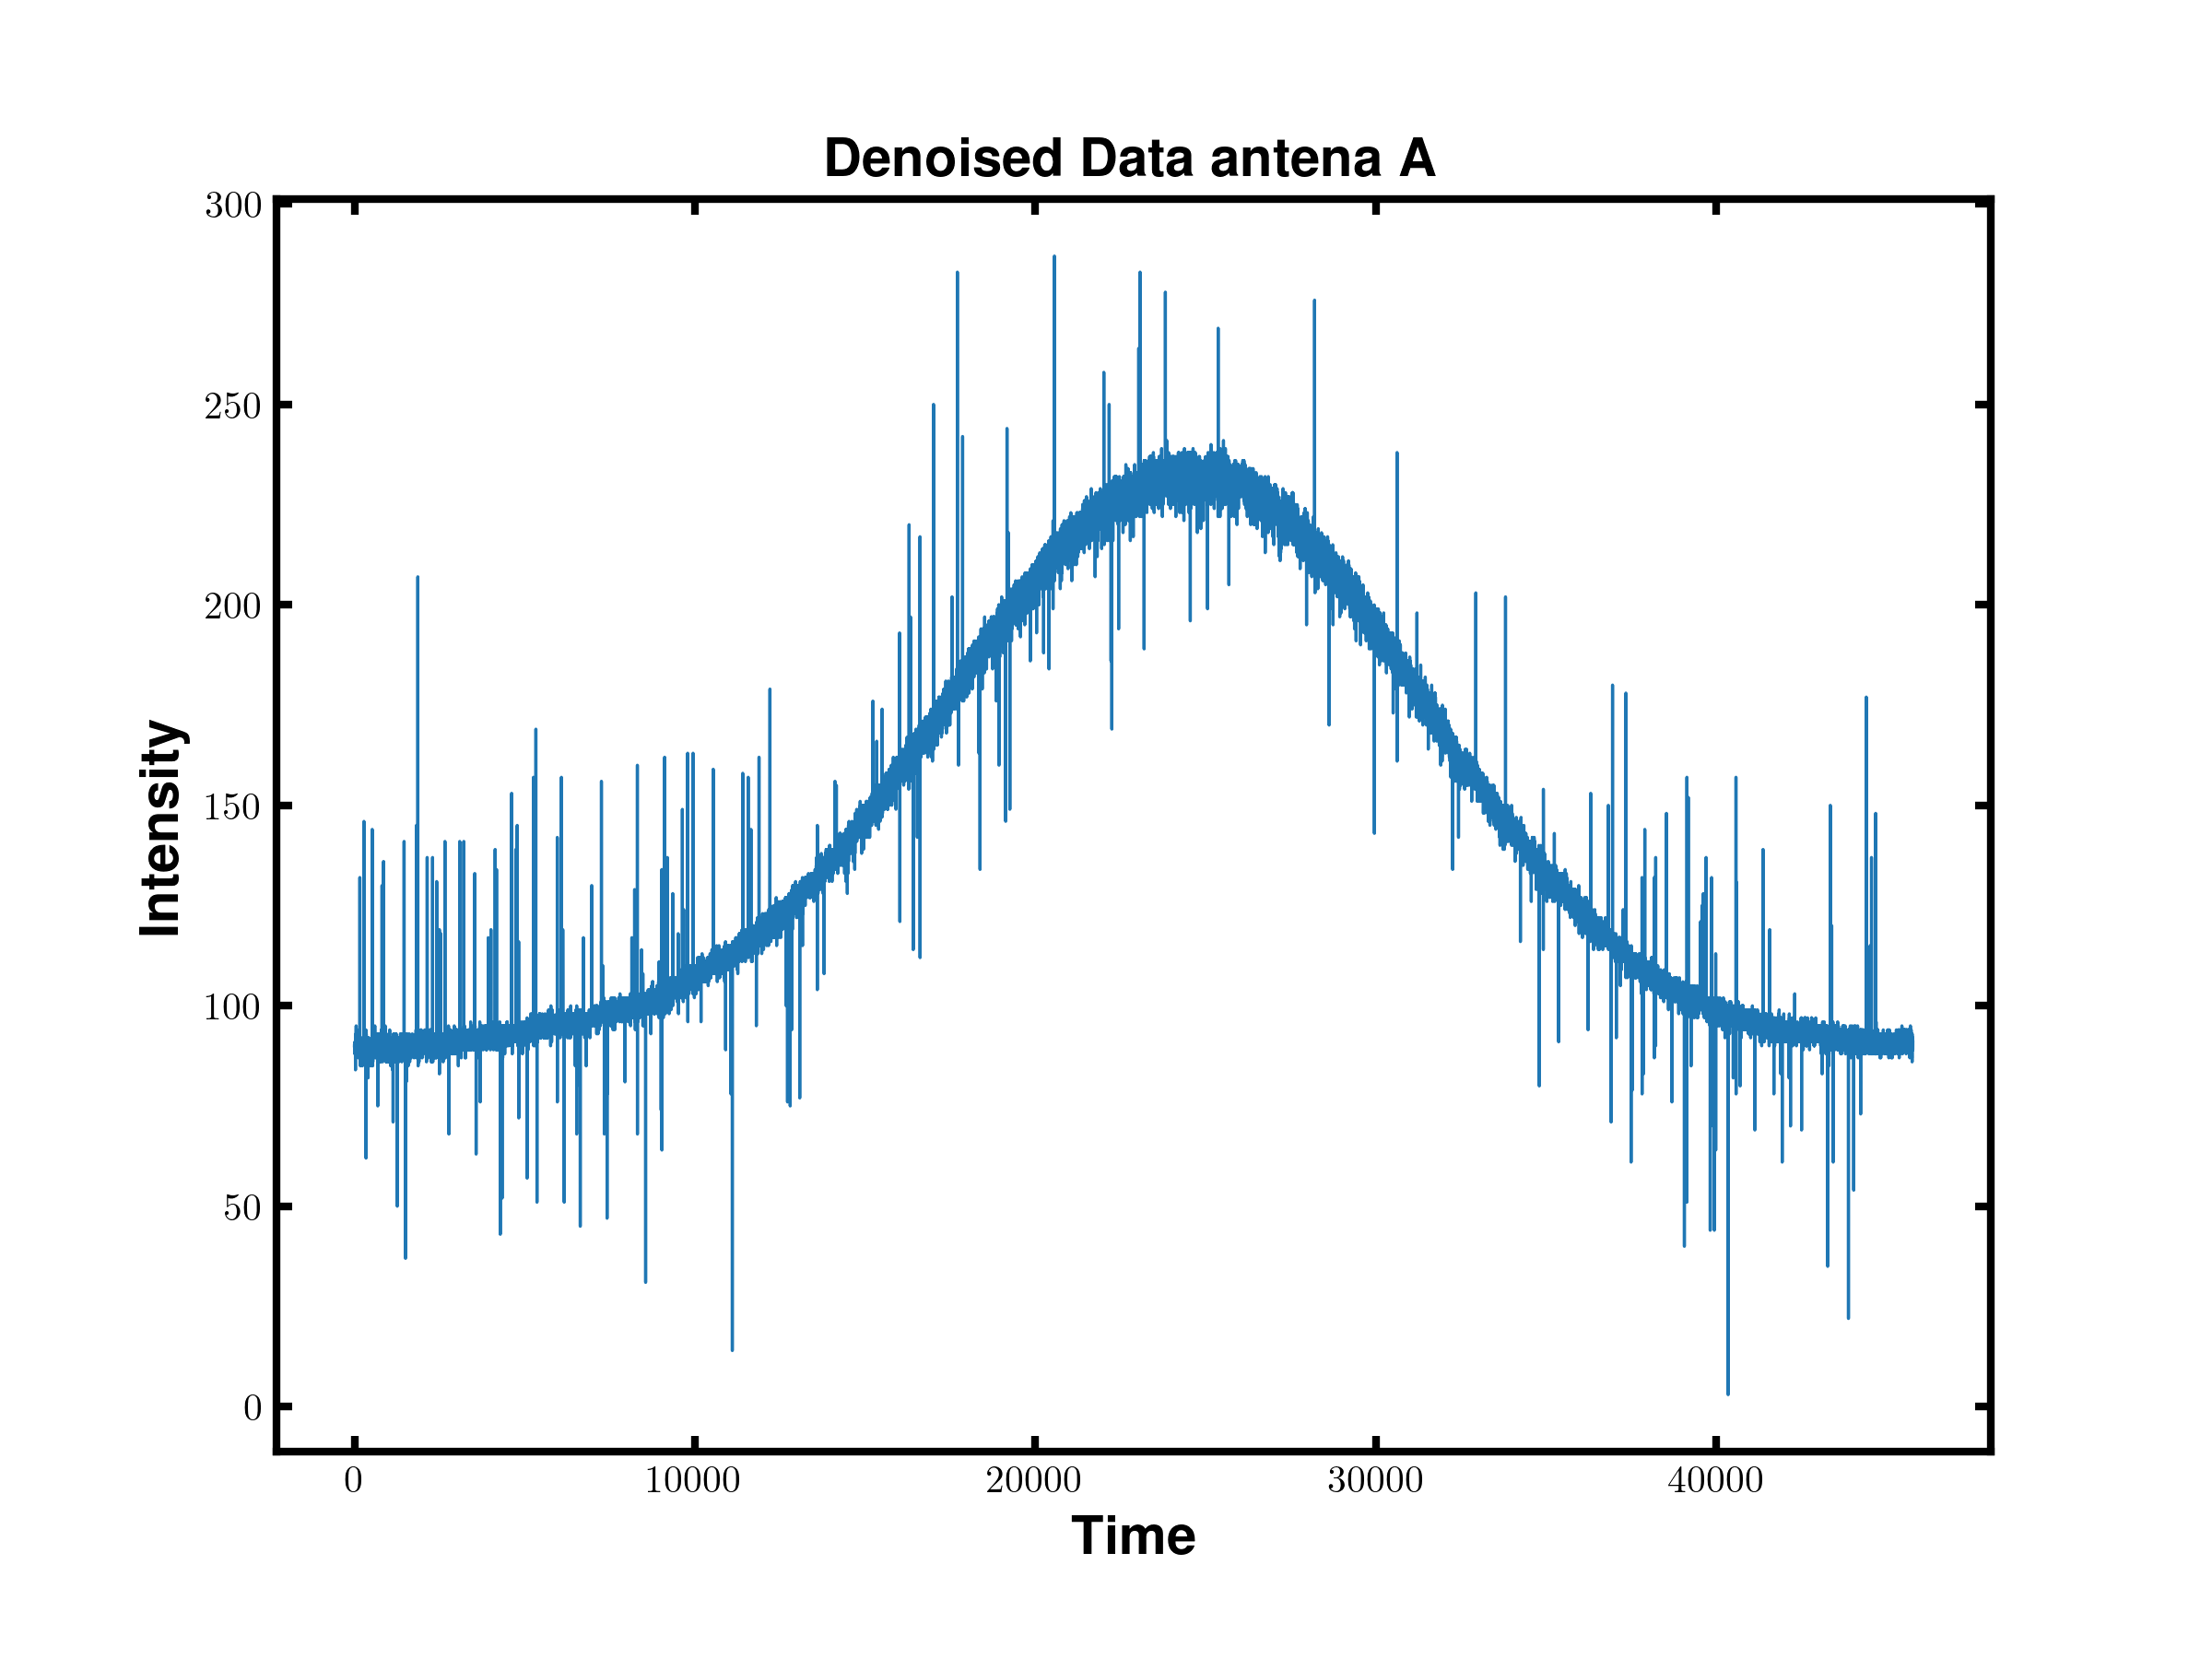
\includegraphics[width=\textwidth]{fig/still_Denoised_Data_antena_A.png}
         \caption{Sun scan antenna A}
         \label{fig2.11}
     \end{subfigure}
     \hfill
     \begin{subfigure}{.45\textwidth}
         \centering
         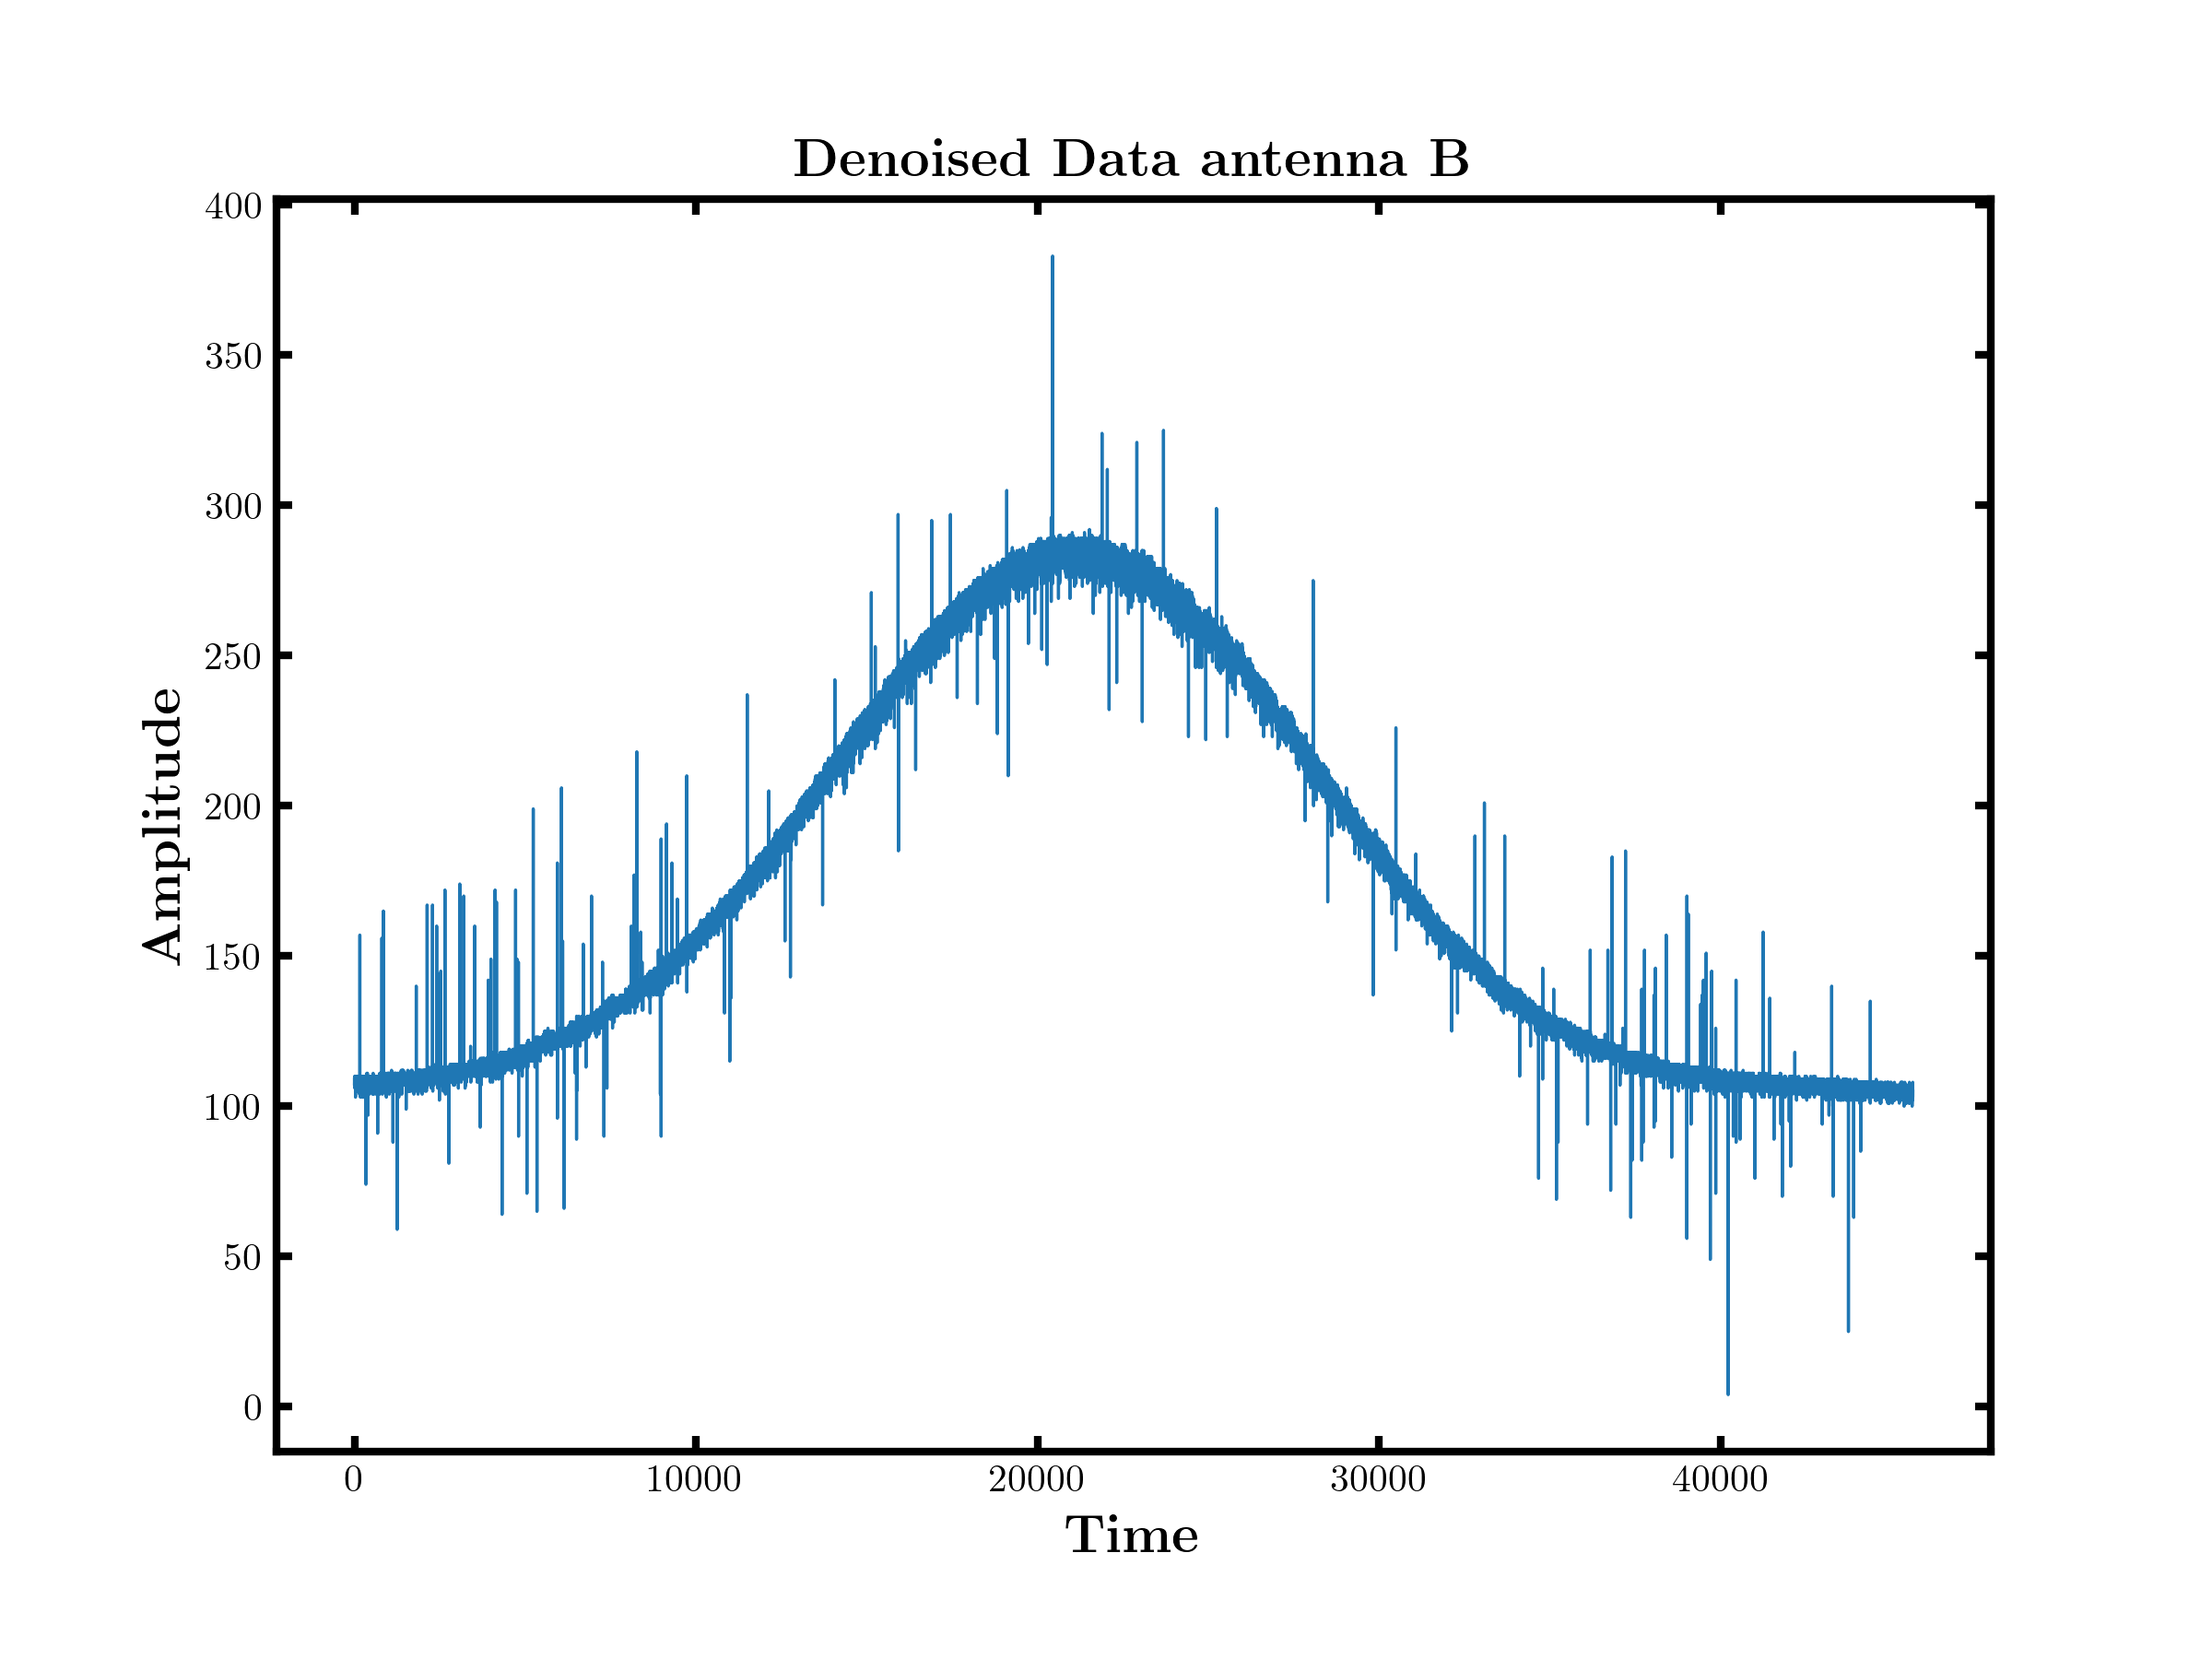
\includegraphics[width=\textwidth]{fig/still_Denoised_Data_antena_B.png}
         \caption{Sun scan antenna B}
         \label{fig2.12}
     \end{subfigure}
        \caption{Intensity vs time plot of the denoised data of the still scan}
        \label{fig2.1112}
 \end{figure}

\section{Error discussion}
\subsection{Setting up a radio-astronomical receiver}
Besides accounting for uncertainties in our analysis, other errors might appear. For example, readings from the HP power meter have also uncertainty as the powermeter only shows one decimal point values, rounding number affects the results of our analysis. In addition, signal interference from the surroundings (e.g noise in the building, or from radars in the city) are inevitable and influence the receiver detection and analysis as a result. A problem with adjusting attenuators was noticed while doing the measurement for exercise 7. We also had a problem with the software in getting the data for exercise 9, we took the data of another team. 

\subsection{Setting up a twin radio interferometer}
There were two primary issues with this configuration. Firstly, the structural integrity of antenna B was weaker compared to antenna A, making it susceptible to deformation under the influence of gravity. This deformation, in turn, led to deviations from the parabolic surface, resulting in unwanted noise in the final output. A deformation larger than $\lambda/10$ causes destructive interference and a shift of the position of focus \cite{klein}. 

Additionally, the alignment procedure relied on using the shadow of the receiver on the antenna's surface. This method is not a best method for alignment and introduced errors in the interference pattern. Although this method is extremely simple and nearly sufficient for this experiment, the error should still be taken into account.


\section{Conclusion}
\subsection{Setting up a radio-astronomical receiver}
A superheterodyne receiver was set up and multiple components were tested to investigate their functionality and linear regimes. A hot-cold calibration was done and the effect of atmospheric attenuation was simulated. Then, the effect of modulating the sensitivity of the receiver was investigated and a radiospectroscopy was done. 
\subsection{Setting up a twin radio interferometer}
In this section, a twin radio interferometer was set up, and it was used to observe the sun. The images of the sun captured with both antennas were used to approximately measure the sun's diameter, and the fringe pattern of the sun was analyzed to determine the angular resolution of the twin radio interferometer. 

\newpage

\printbibliography
\end{document}